\documentclass[11pt,a4paper,oneside]{article}             % Single-side
%\documentclass[11pt,a4paper,twoside,openright]{report}  % Duplex

%\PassOptionsToPackage{chapternumber=Huordinal}{magyar.ldf}
%\usepackage{t1enc}
\usepackage[T1]{fontenc}
\usepackage[utf8]{inputenc}
\usepackage{amsmath}
\usepackage{amssymb}
\usepackage{enumerate}
\usepackage[thmmarks]{ntheorem}
\usepackage{graphics}
\usepackage{epsfig}
\usepackage{listings}
\usepackage{color}
%\usepackage{fancyhdr}
\usepackage{lastpage}
\usepackage{anysize}
%\usepackage[magyar]{babel}
\usepackage{sectsty}
\usepackage{setspace}  % Ettol a tablazatok, abrak, labjegyzetek maradnak 1-es sorkozzel!
\usepackage[hang]{caption}
\usepackage{hyperref}
\usepackage{wrapfig}
\usepackage{tcolorbox}
\usepackage{float}

%--------------------------------------------------------------------------------------
% Main variables
%--------------------------------------------------------------------------------------
\newcommand{\vikszerzo}{Fodor Attila}
\newcommand{\vikkonzulens}{Kundra László}
\newcommand{\vikcim}{Autonóm oceanográf}
\newcommand{\viktanszek}{Department of Automation and Applied Informatics}
\newcommand{\vikdoktipus}{Diplomaterv}
\newcommand{\vikdepartmentr}{Fodor Attila}

%--------------------------------------------------------------------------------------
% Page layout setup
%--------------------------------------------------------------------------------------
% we need to redefine the pagestyle plain
% another possibility is to use the body of this command without \fancypagestyle
% and use \pagestyle{fancy} but in that case the special pages
% (like the ToC, the References, and the Chapter pages)remain in plane style

\floatstyle{boxed}

\pagestyle{plain}
\setlength{\parindent}{0pt} % áttekinthetőbb, angol nyelvű dokumentumokban jellemző
\setlength{\parskip}{8pt plus 3pt minus 3pt} % áttekinthetőbb, angol nyelvű dokumentumokban jellemző
%\setlength{\parindent}{12pt} % magyar nyelvű dokumentumokban jellemző
%\setlength{\parskip}{0pt}    % magyar nyelvű dokumentumokban jellemző

\marginsize{35mm}{25mm}{15mm}{15mm} % anysize package
\setcounter{secnumdepth}{0}
\sectionfont{\huge\upshape\bfseries}
\setcounter{secnumdepth}{0}
\singlespacing
\frenchspacing

%--------------------------------------------------------------------------------------
%	Setup hyperref package
%--------------------------------------------------------------------------------------
\hypersetup{
    bookmarks=true,            % show bookmarks bar?
    unicode=false,             % non-Latin characters in Acrobat’s bookmarks
    pdftitle={\vikcim},        % title
    pdfauthor={\vikszerzo},    % author
    pdfsubject={\vikdoktipus}, % subject of the document
    pdfcreator={\vikszerzo},   % creator of the document
    pdfproducer={Producer},    % producer of the document
    pdfkeywords={keywords},    % list of keywords
    pdfnewwindow=true,         % links in new window
    colorlinks=true,           % false: boxed links; true: colored links
    linkcolor=black,           % color of internal links
    citecolor=black,           % color of links to bibliography
    filecolor=black,           % color of file links
    urlcolor=black             % color of external links
}

%--------------------------------------------------------------------------------------
% Set up listings
%--------------------------------------------------------------------------------------
\lstset{
	basicstyle=\scriptsize\ttfamily, % print whole listing small
	keywordstyle=\color{black}\bfseries\underbar, % underlined bold black keywords
	identifierstyle=, 					% nothing happens
	commentstyle=\color{white}, % white comments
	stringstyle=\scriptsize\sffamily, 			% typewriter type for strings
	showstringspaces=false,     % no special string spaces
	aboveskip=3pt,
	belowskip=3pt,
	columns=fixed,
	backgroundcolor=\color{lightgray},
} 		
\def\lstlistingname{lista}	

%--------------------------------------------------------------------------------------
%	Some new commands and declarations
%--------------------------------------------------------------------------------------
\newcommand{\code}[1]{{\upshape\ttfamily\scriptsize\indent #1}}

% define references
\newcommand{\figref}[1]{\ref{fig:#1}.}
\renewcommand{\eqref}[1]{(\ref{eq:#1})}
\newcommand{\listref}[1]{\ref{listing:#1}.}
\newcommand{\sectref}[1]{\ref{sect:#1}}
\newcommand{\tabref}[1]{\ref{tab:#1}.}

\DeclareMathOperator*{\argmax}{arg\,max}
%\DeclareMathOperator*[1]{\floor}{arg\,max}
\DeclareMathOperator{\sign}{sgn}
\DeclareMathOperator{\rot}{rot}
\definecolor{lightgray}{rgb}{0.95,0.95,0.95}

\author{\vikszerzo}
\title{\viktitle}

%--------------------------------------------------------------------------------------
%	Setup captions
%--------------------------------------------------------------------------------------
\captionsetup[figure]{
%labelsep=none,
%font={footnotesize,it},
%justification=justified,
width=.75\textwidth,
aboveskip=10pt}

\renewcommand{\captionlabelfont}{\small\bf}
\renewcommand{\captionfont}{\footnotesize\it}

%--------------------------------------------------------------------------------------
% Table of contents and the main text
%--------------------------------------------------------------------------------------
\begin{document}
\singlespacing

\pagenumbering{arabic}
\onehalfspacing
%--------------------------------------------------------------------------------------
%	The title page
%--------------------------------------------------------------------------------------
\begin{titlepage}
\begin{center}

\includegraphics[width=60mm,keepaspectratio]{figures/BMElogo.png}\\
\vspace{0.3cm}
\textbf{Budapesti Műszaki és Gazdaságtudomái Egyetem}\\
\textmd{Villamosmérnöki és Informatikai Kar}\\
\textmd{\viktanszek}\\[5cm]

\vspace{0.4cm}
{\huge \bfseries \vikcim}\\[0.8cm]
\vspace{0.5cm}
\textsc{\Large \vikdoktipus}\\[4cm]

\begin{tabular}{cc}
\makebox[7cm]{\emph{Készítette}} & \makebox[7cm]{\emph{Konzulens}} \\
\makebox[7cm]{\vikszerzo} & \makebox[7cm]{\vikkonzulens}
\end{tabular}

\vfill
{\large \today}
\end{center}
\end{titlepage}



\tableofcontents\vfill
%%--------------------------------------------------------------------------------------
% Nyilatkozat
%--------------------------------------------------------------------------------------
\begin{center}
\large
\textbf{HALLGATÓI NYILATKOZAT}\\
\end{center}

Alulírott \emph{\vikszerzo}, szigorló hallgató kijelentem, hogy ezt a szakdolgozatot/ diplomatervet \textcolor{blue}{(nem kívánt törlendő)} meg nem engedett segítség nélkül, saját magam készítettem, csak a megadott forrásokat (szakirodalom, eszközök stb.) használtam fel. Minden olyan részt, melyet szó szerint, vagy azonos értelemben, de átfogalmazva más forrásból átvettem, egyértelműen, a forrás megadásával megjelöltem.

Hozzájárulok, hogy a jelen munkám alapadatait (szerző(k), cím, angol és magyar nyelvű tartalmi kivonat, készítés éve, konzulens(ek) neve) a BME VIK nyilvánosan hozzáférhető elektronikus formában, a munka teljes szövegét pedig az egyetem belső hálózatán keresztül (vagy autentikált felhasználók számára) közzétegye. Kijelentem, hogy a benyújtott munka és annak elektronikus verziója megegyezik. Dékáni engedéllyel titkosított diplomatervek esetén a dolgozat szövege csak 3 év eltelte után válik hozzáférhetővé.

\begin{flushleft}
\vspace*{1cm}
Budapest, \today
\end{flushleft}

\begin{flushright}
 \vspace*{1cm}
 \makebox[7cm]{\rule{6cm}{.4pt}}\\
 \makebox[7cm]{\emph{\vikszerzo}}\\
 \makebox[7cm]{hallgató}
\end{flushright}
\thispagestyle{empty}

\vfill
\clearpage
\thispagestyle{empty} % an empty page


%----------------------------------------------------------------------------
% Abstract in hungarian
%----------------------------------------------------------------------------
%\chapter*{Kivonat}\addcontentsline{toc}{chapter}{Kivonat}
\section{Kivonat}

Jelen dokumentum egy diplomaterv sablon, amely formai keretet ad a BME Villamosmérnöki és Informatikai Karán végző hallgatók által elkészítendő szakdolgozatnak és diplomatervnek. A sablon használata opcionális. Ez a sablon \LaTeX~alapú, a \emph{TeXLive} \TeX-implementációval és a PDF-\LaTeX~fordítóval működőképes.
\vfill

%----------------------------------------------------------------------------
% Abstract in english
%----------------------------------------------------------------------------
%\chapter*{Abstract}\addcontentsline{toc}{chapter}{Abstract}
\section{Abstract}

This document is a \LaTeX-based skeleton for BSc/MSc~theses of students at the Electrical Engineering and Informatics Faculty, Budapest University of Technology and Economics. The usage of this skeleton is optional. It has been tested with the \emph{TeXLive} \TeX~implementation, and it requires the PDF-\LaTeX~compiler.
\vfill


%\chapter*{Introduction}\addcontentsline{toc}{chapter}{Introduction}
\section{Introduction}

Seaborne measurements are often expensive and time consuming, though they can have a large impact on the area, where the data have been obtained. In 2011 the naval safe zone around the Fukusima accident was laid down based only on estimates of the radiation contamination\cite{FNPP}, because low amount of measurement data was available due to high measurement costs and risks. Another notable example are the coastal waters of Greenland, because are very poorly mapped up to present day\cite{2009AGUFMOS21A1152W}. Ships have to sail in a roundabout way around the island, because the risk of wrecking in unknown fjordic area is very high. This is a huge waste of time and natural resources annually.

\subsection*{Oceanography and Bathymetry}

Not many people come across these expressions often. Oceanography can be summarized as a branch of Earth science that studies the ocean. It includes a wide range of topics, like the study of marine ecosystem, ocean currents, plate tectonics and the geology of the sea floor. Bathymetry is the study of underwater depth of lake or ocean floors. The advancing technology allows even more possibilities, like the aforementioned radiological measurements, or general monitoring of the seas.

\subsection{Advantages of autonomous vessels}

Oceanographic measurements today are carried out by large crewed ships, but in many cases they could be replaced by a number of smaller crafts, in order to reduce surveying time and cost and increase the available manpower in other tasks. These vessels could have the ability to sail previously unsurveyable areas as well, thanks to the shallower draught and smaller size.

\subsection{Limitations}

The most notable limitation of the current mobile robotic technologies are their small size itself. It means the relatively small range based on their smaller power capabilities, and narrow field of application.

The aim of this project is to develop an autonomous surface vehicle, which is capable of conducting multiple seaborne measurements. To execute an oceanography mission, the ship must be capable of autonomus navigation based on Global Positioning System (GPS) and an Internal Measurement Unit (IMU), to further enhance the precision in hazardous environment.

\begin{figure}[H]
	\centering
	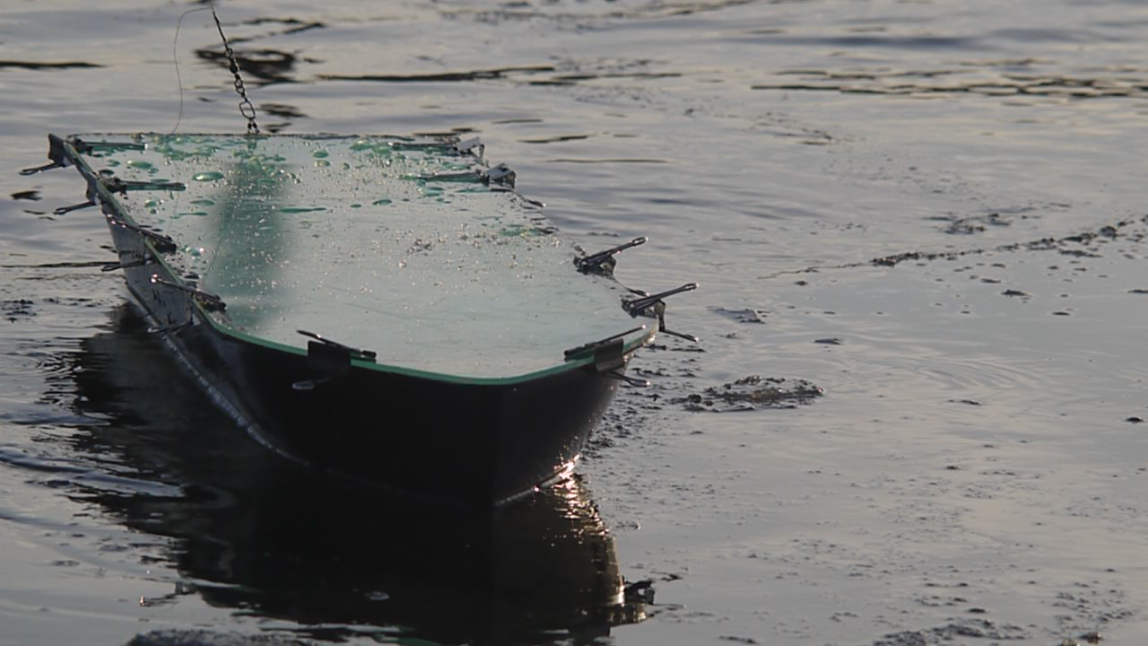
\includegraphics[width=0.8\textwidth]{img/aauship}
	\caption{The AAUSHIP prototype on her maiden voyage}
	\label{fig:aauship}
\end{figure}

\subsection*{Development guidelines}
In order to keep a sensible and extendable system, the control software of the ship follows the guidelines of the Model-Based Design approach. The system software can be divided to two different kind of modules, one that is dependent, and one that is independent from the physical characteristics of the vessel. In order to maximize the extendability of the system, the fix (independent) modules must be completely general, but as thorough as possible, so as to keep the complexity of the changeable (dependent) software of the robot minimal.
\begin{wrapfigure}{r}{0.48\textwidth}
  \begin{center}
    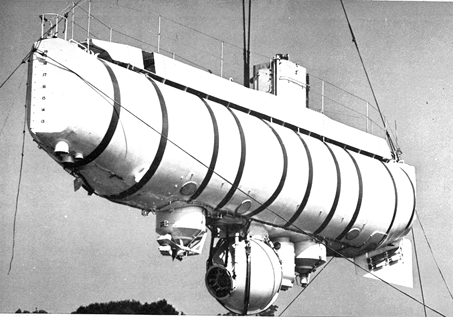
\includegraphics[width=0.5\textwidth]{img/trieste}
  \end{center}
  \caption{Bathyscaphe Trieste, the first manned vessel that reached the bottom of Challenger Deep (Mariana Trench)\cite{trieste}}
\end{wrapfigure}

The environment stored in the control system must be extendable to the third dimension, and must be able to track changes over time.
The tasks of the low level control must be as specific and as basic as possible. All calculations and control should be implemented in the high level controller.
the high level controller must be parametrized, based on the low level and hardware characteristics.

The point of these guidelines is to create a system of components with major reusability. Ideally a general Cross-platform High Level Controller controls different kind of vessels, through a standard interface. When changing to an arbitrary different vehicle, only the Low Level Controller must be replaced, which stores the characteristics of the vessel and implements the actuator control.

\section*{Operation models}

 A typical oceanography application starts on the shore. A science team analyzes the currently available data, then marks the area of measurements on the map. The  map data is transformed to a measurement path by the scientists or by the automatic waypoint planner of the ship. The autonomous surface vehicle is then outfitted with the right sensors for the task, and a manned ship transports it close to its destination. The crew can set the research vessel to manual, automatic or fully autonomous mode.

\paragraph{Manual control}
In this mode it's possible for the operator to control the movement of the ship, degree of freedom-wise or control the actuators themselves. The primary intent of this mode is for testing or malfunction-recovery.

\begin{figure}[H]
	\centering
	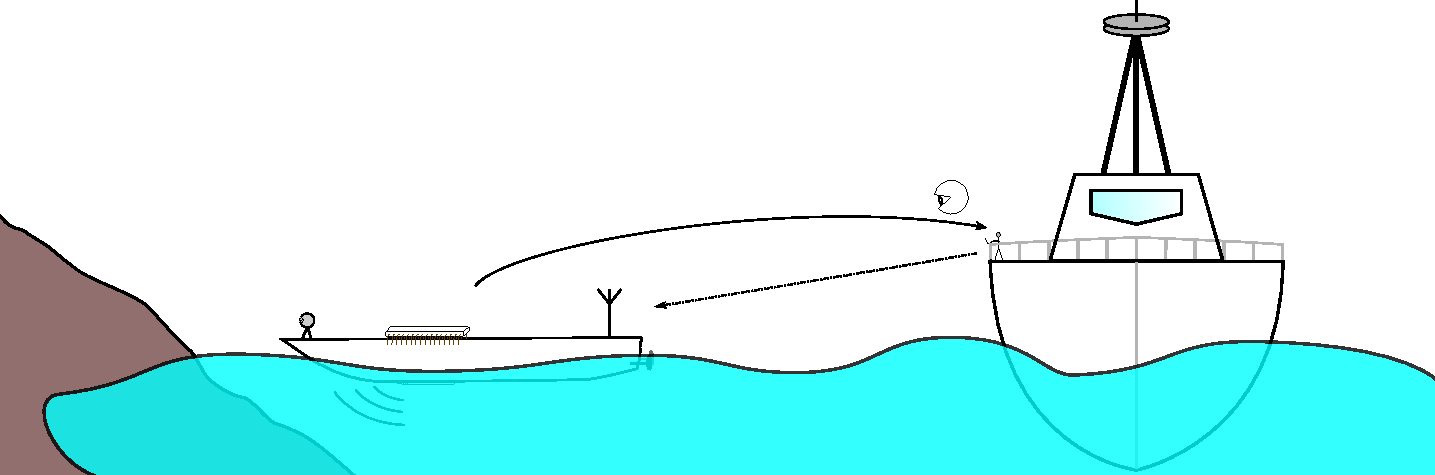
\includegraphics[width=0.8\textwidth]{img/manualcontrol}
	\caption{Manual remote control}
	\label{fig:manualcontrol}
\end{figure}

\paragraph{Automatic control}
In automatic mode the "brains", remain on the crewed vessel, and the research craft remains in wireless connection with the Mothership. When the measurements are complete, the oceanographer returns to the mothership. In automatic mode it is always possible to switch to manual control and back, or update the measurement path, etc.

\begin{figure}[H]
	\centering
	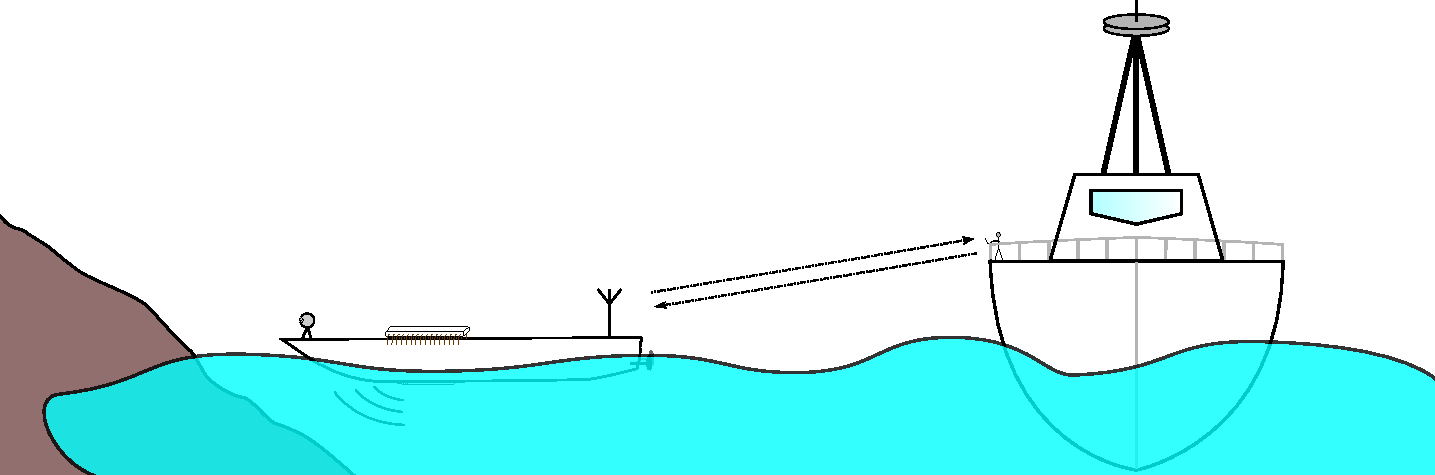
\includegraphics[width=0.8\textwidth]{img/automatic}
	\caption{Automatic supervised control}
	\label{fig:automatic}
\end{figure}

\paragraph{Autonomus control}
In Autonomus mode the ship carries everything that is needed to complete the task. Connection to the mothership can be cut, and the vessel carries the orders out autonomusly. Intervention in this mode is only possible until the oceanographer is in range of the mothership.

\begin{figure}[H]
	\centering
	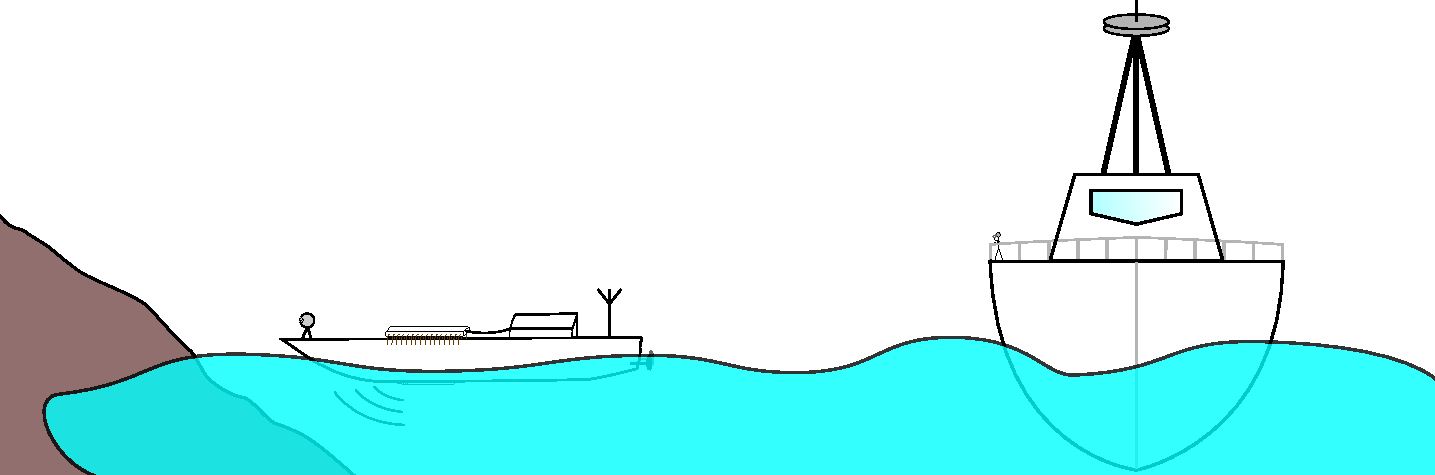
\includegraphics[width=0.8\textwidth]{img/autonomus}
	\caption{Autonomus control}
	\label{fig:autonomus}
\end{figure}

\paragraph{}
In case there are multiple research vessels, they can form a squadron. In this setup only one of the ships needs to be in range of the crewed mothership. Alternatively one autonomus ship is capable of controlling multiple automatic crafts, taking over the role of the mothership.

\begin{figure}[H]
	\centering
	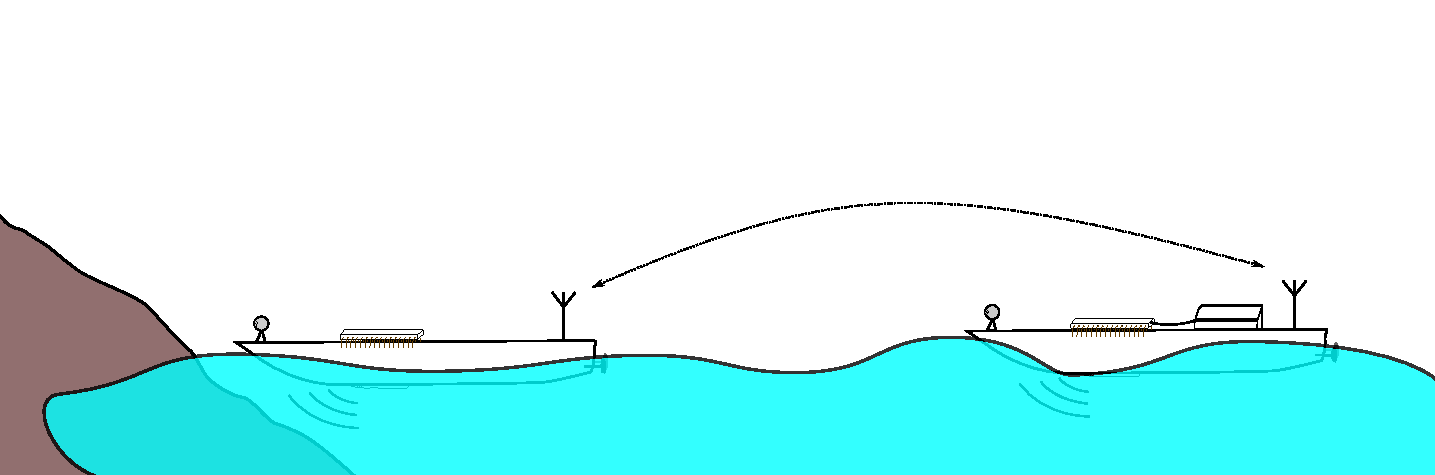
\includegraphics[width=0.8\textwidth]{img/multiple}
	\caption{Squadron mode}
	\label{fig:multiple}
\end{figure}

\begin{tcolorbox}[colback=cyan!5,colframe=cyan!40!black,title=Code: Main.py \\ https://www.dropbox.com/s/h1067ywmdajkegk/Main.py]
\begin{minipage}{0,6\textwidth}
The mission planning steps are implemented in Main.py, which is the main part of the program, responsible for initializing the system, setting the target area, mode of routing, navigation, etc. Later Main.py will provide a Graphical User Interface as well.
\end{minipage}
\begin{minipage}{0,35\textwidth}
\raggedleft

\includegraphics[width=0.8\textwidth]{img/main}
\end{minipage}

\end{tcolorbox}

%\chapter*{Operational Requirements}\addcontentsline{toc}{chapter}{Operational Requirements}
\section{Operational Requirements}

\subsection{General requirements of autonomus vehicles}

\subsection{Requirements of survey ships}

\subsection{Combined requirements}

In order to execute a rational oceanography task, a number of valid objectives must be set. These objectives are usually one or more of the following\cite{oceanography}:

\begin{itemize}
\item A set of geographical measurement locations, with or without time and measurement type conditions
\item A certain area of interest
\item Maximal action duration requirement
\item Other
\end{itemize}

The task planning is usually carried out by the scientist group, but some auto-planning modes need to be supported. A typical task is the creation of a measurement-grid, with preset definition, in a certain geographical area. The High Level Controller (HLC) uses a Mission planning time algorithm, to support the auto-generation of the waypoints. This module is the "Waypoint planner", which outputs a list of coordinates that contains the measurement points.

Once the ship reaches the current waypoint, it determines the next aim.

A set of points defining a path can be specified for the ship, but it does not ensure that the created path is valid, therefore a second "Pathplanning" stage is required, which analyzes the generated set of locations and creates a path that is actually sailable by the ship.
\section{Common ship body and propulsion types}

Throughout history, countless ship types have been brought to life, due to the various and ever-changing environmental challenges they had to overcome. Therefore they can be grouped or ordered several different ways, based on their shape, propulsion, area of application, origin and so forth. Modern ships have introduced remarkably advanced propulsion technologies, and even more are still in development. This section will give a quick overview about the most widespread possibilities, but the thesis will analyze only some of them.

\subsection{Hull types}

The lore of shipbuilding/footnote{Just like many other scholars of ancient history, early masters of shipbuilding were considered artists \cite{Art_of_shipbuilding}} is centered around the design of the hull, and it's probably a sensible way to start categorizing ships.
The fundamental concept of a ship hull design is the low resistance along the direction of forward motion. A lower drag results in faster top speed and lower energy requirements. Lateral shape is only mildly important in the design of self propelled ships, however sailing with side-wind is only possible by balancing the front and lateral resistances carefully\cite{vitorlazas}.

\paragraph{Lateral surface} affects the ability of the ship to sail and turn. A high lateral surface results in good wind-response but generally decreases the turning agility and increases the frontal surface and friction.

\subsection{Stability of a ship} 

Stability is the ability of the vessel to return to it's previous position\cite{stability}. This righting movement is the result of the relationship between the \textbf{Center of Mass} (CoG), and the \textbf{Center of Buoyancy} (CoB) of the ship. The stability can be divided to three different movements, independent from each other.

\paragraph{Static stability} is the stability at rest, without any external forces. In contrary to the CG, which is a point fixed to the body of the ship\footnote{Unless the ship features moving ballast, like the sailor of a dinghy}, the CoG constantly changes it's position as the ship heels or trims. If the CoB and CoG don't align vertically, the ship keeps changing it's attitude, until they do.

\begin{figure}[H]
	\centering
	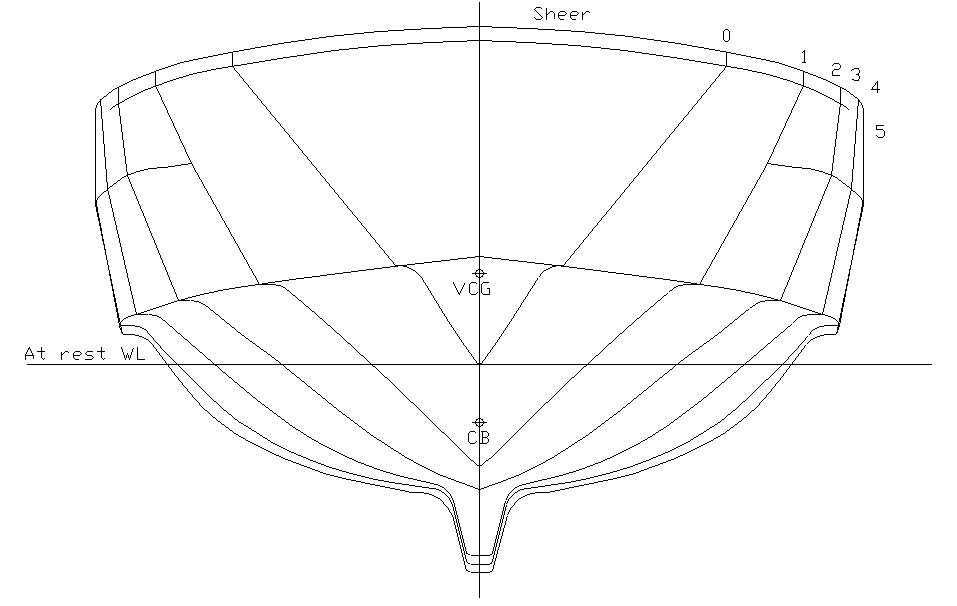
\includegraphics[width=0.6\textwidth]{img3/stability0}
	\caption{Static stability of a still boat\\http://www.brayyachtdesign.bc.ca/}
	\label{fig:stability0}
\end{figure}

\paragraph{Form stability} As the boat moves, some area submerges, some reveals from the water. As the hull is heeling, the CoB moves, and depending on the form stability the boat will either overturn, or enough counter-tourqe will build up to reverse the tilting motion.

\begin{figure}[H]
	\centering
	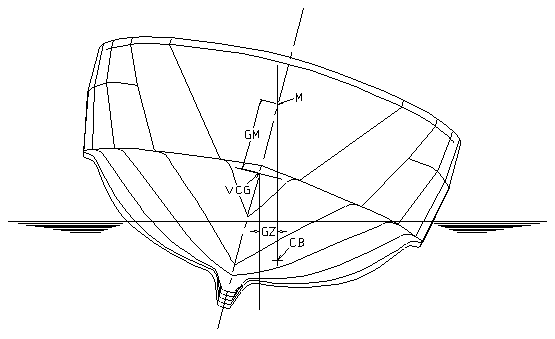
\includegraphics[width=0.6\textwidth]{img3/stability1}
	\caption{Form stability of a heeling boat\\http://www.brayyachtdesign.bc.ca/}
	\label{fig:stability1}
\end{figure}

\paragraph{Dynamic stability} is generated when the ship is moving, and the effect is increased with speed. The dynamic stability can either increase or decrease the overall stability, but most modern boats are considerably more stable at higher speeds, due to special hull shaping. As the pressure increases under the hull, the dynamic forces will become stronger compared to the effects of buoyancy, and a round-bottomed hull can become unstable, as the width and shape of the hull beneath the water is significantly narrower than during static buoyancy.

\begin{figure}[H]
	\centering
	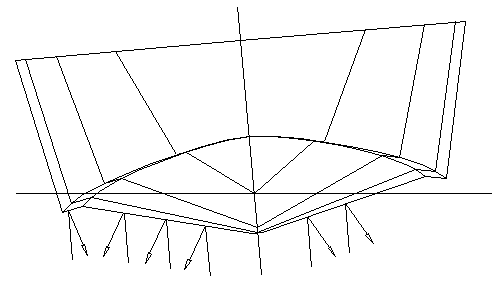
\includegraphics[width=0.6\textwidth]{img3/stability2}
	\caption{Dynamic stability of a speeding boat\\http://www.brayyachtdesign.bc.ca/}
	\label{fig:stability2}
\end{figure}

\paragraph{Stability in general} It's notable, that even though a boat with high form and dynamic stability can offer a pleasant still water comfort, also provides a very rough ride at higher speeds, due to the quick hull reactions. On the contrary, a smooth wave-cutter promises constant swaying and vertical movement in a harbor.

One of the earliest efforts to increase stability was the extra \textbf{Ballast} added to the bottom of the ship, ranging from a couple of rocks to a keel mounted metal fin. The principle of the ballast is to lower the center of gravity. Many modern sailboats feature a lower CoG than the CoB therefore becoming immune to capsizing. Even after a complete turnover, the boat will eventually return to it's original state\footnote{Given that no structural damage happened during this undesirable event}.
Another, but considerably different effort to ensure stability is a wide \textbf{Beam}ed hull. While the ballast provides good ultimate stability, it lacks the initial stability, and the body can gather up quite some tilt until the gravity starts working. Contrary to the ballast, a wide beam provides good initial stability but does not provide the righting movement after a certain point. However,  wide beam monohulls can be dangerous, because it reaches the peak of initial stability quickly and the ship is more likely to capsize, but multihulls\footnote{Catamarans, trimarans} can boast exceptional stability qualities.

\begin{figure}[H]
	\centering
	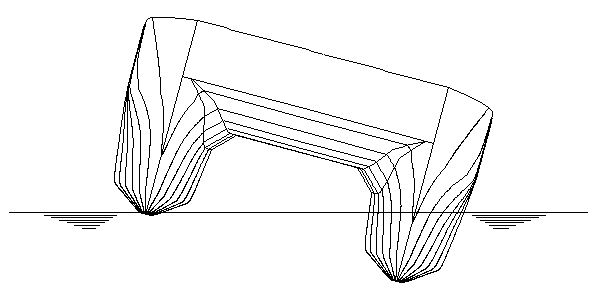
\includegraphics[width=0.6\textwidth]{img3/stability3}
	\caption{Wide beam multihull boat\\http://www.brayyachtdesign.bc.ca/}
	\label{fig:stability3}
\end{figure}

The response speed of the ship can be adjusted by the placement of equipment and cargo on the ship. By moving weight away from the centerline horizontally, the increased \textbf{inertia} dampens the quick movements caused by high initial stability. If a ship is close to turning over completely, a well-designed \textbf{Superstructure} can still have a positive impact on the stability, and save the day. Unfortunately, a large superstructure is effected by heavy winds, which can be a problem, if the ship lacks a good stability.

In conclusion, adequate stability can be ensured with common sense during the design process, but an all round stability is the result of careful planning.

\paragraph{Sailing rigg} 

Many centuries had to pass until humanity discovered the way to sail sideways to the wind, and even towards the wind in some degree. Modern sailboats still provide a good alternative to motorised ships especially in still water. Contrary to the belief, sailing ships are not the only wind powered ships currently existing, although they proved to be the most efficient. However, Rotor ships are still manufactured, mostly as part of a hybrid propulsion system.

Wrapfig Here.

Regulations in the European Union even prevent the usage of petrol engine in Lakes unless sailing in the harbour or under hazardous conditions, and sailboats are still popular for recreational use. The sails, the mast, the ropes and other similar equipment are all part of the rig. The rigging has many various forms depending on the number of masts, size of the ship and the type of sails. The most widespread type of mother and sailing yachts is the single masted rig width to triangular sails. The fore-sail  is fixed while the mainsail can be rotated with the boom. There are a lot of additional sail types, especially on the racing boats. Most common of them is the spinnaker, which is a large parabolic sail used for reaching, often featuring colorful graphics.

\paragraph{Mechanized propeller propulsion}

Every ship, even before the steam engine was invented featured some sort of mechanical propulsion, most notably galleys. Modern yachts offer petrol or electric engines for either main or supplementary driving. In case of smaller boats the drive train consists of a shaft connected to the engine, a propeller and a rudder. Jet propulsion, which only the fastest sports and jetskis feature is less common, because they sacrifice efficiency for speed.
Large ships and submarines are often outfitted width a nuclear power plant, although for different reasons. In case of large vessels the primary motivation is the almost unlimited range, because a nuclear reactor can provide enough power to keep the ship on the sea for a long time, and the replenishment of fuel has become much smaller problem. On the contrary the primary advantage of the nuclear engines in a submarine is the fact that it doesn't require air for the power production process. The underwater range of early submarines were limited because they had to emerge from time to time to the surface where they are exposed to detection and enemy fire.

\subsection{Design conclusions}

In case of a civilian unmanned surface vehicle many problems described above can be ignored because of the small size of the boat, the lack of human crew and non-military application.
Stability is very important in case of sailing vessels, because stronger wind can create a large torque on the ship. Single and multihull vessels respond to this torque entirely differently. The single hull boat is stabilised by a keel mounted ballast that provides low initial stability, the boat will heel and the effective sail size will reduce, but ultimately will remain stable. On the contrary, a multi-hull ship featuring high initial stability will respond with rapidly increasing speed. This characteristic has made catamarans and especially trimarans very popular among racers, but they carry the dangers of tripping over, and the writing of a capsized trimaran is hardly possible without external help. In conclusion, a  trimaran can easily outperform a classic sailboat in terms of speed and agility, but they can be used safely in a controlled environment only. On the other hand a single-hull boat with a weighted keel and sufficiently watertight inner compartments is much more reliable in the harsh environment of an ocean.

During the thesis two different ships types will be designed. The first vessel is a short range electric motorised boat, featuring a multi-hull trimaran design. Primary application areas are short missions requiring high agility and quick mobilisation (Codename: Kestrel). The second is a single-hull sailboat capable of conducting long-range measurements where regular maintenance is impossible and high reliability must be ensured (Codename: Stork).


\section{Dynamic models of ships}

Simple ship dynamic models can be formulated quickly by defining and analyzing the most common propulsion methods. However, these are only vague approximations of the system, and contain few elements of the complex and powerful hydrodynamics.

First the simple ship models are introduced, then an attempt is made to more accurately describe the dynamical system of a ship.

\subsection{Differential drive}

The differential drive system is very common among simple mobile robotic systems. The movement is based on two separately driven wheels placed on either side of the robot body. It can thus change its direction by varying the relative rate of rotation of its wheels, therefore does not require an additional steering mechanism. A twin-screw ship has a somewhat similar layout. Using the engines positioned in a lateral offset to the centerline of the body, the ship can create a torque and propelling force affecting the body.

\begin{figure}[H]
	\centering
	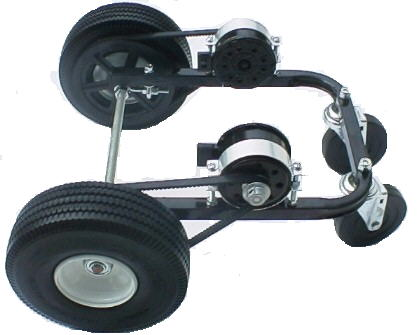
\includegraphics[width=0.8\textwidth]{pics/kadtronixframe}
	\caption{Differential drive robot frame \\ http://www.kadtronix.com/}
	\label{fig:kadtronixframe}
\end{figure}

This type of ship can be modeled as a 2-DOF mobile robot (frame fixed to the body of the ship).

The dynamical system of the parallel propulsion engines can be formulated easily:


Figure here! d is the distance of the wheel from the center

\begin{align}
	\dot{x} &= \frac{v_1}{2} + \frac{v_2}{2} \\
    \dot{\Theta} &= \frac{v_1-v_2}{2*d}
\end{align}

From a control engineer’s point of view the most important aspect of this control system is its linearity. Designing a basic controller for this type of robot is a walk in the park.

The mechanical advantage of this layout is the very high reliability, because the propellers are fixed in a certain angle, therefore they can be build more roboustly, thus decreasing the chance of physical failture. Another advantage is the ability of the ship to turn around it’s central axis, enabling precise maneuvering, however, this is seldom used, because it’s very ineffective with ships.
Usually older large container-ships employ this type of propulsion. Newer large-scale ship design have kept the multi-screw layout, but also included a rudder directly after the propellers to enhance turning.

\subsection{Rudder ship}

The rudder is a controllable part of the ship, creating a tourque on the body of the ship, using hydrodynamical effects, much like the rudders of airplanes. The generated torque depends on the traveling speed. The ship can not rotate around it’s center axis.

The rudder ship can be modeled as a car with Euler(?) steering.

\begin{align}
	\dot{x} &= v \\
	\dot{\Theta} &= \frac{v * tan(\Phi)}{L}
\end{align}

This control type is usually fitted on faster ships, exploiting the possibility to create high torques on the body at high speeds, resulting in sharp turns.

\subsection{Sailing ship}

The sailing ship is usually a rudder controlled ship, but it’s possible to alter the course of a sailing vessel by adjusting the sales or tilting the mast (e.g.: windsurfing).
There are many forces affecting the sails and the body of the ship, but it’s way out of the scope of this text to model all of them. However, they can be generalized in two forces, the lift and the drag.

Lift is the force generated on the saild by the wind, affecting paralell with the body of the ship, and drag is the force generated perpendicular to the body of the ship. These forces are greatly and nonlinearly dependent on the strength and direction of the wind, current speed, air pressure, wind shears, local temperature gradiants and a lot of other circumstances.

However, they allow to generalize the system into a 3-dof system after making the following assumptions:

The relative wind is the vectorial subtraction of the velocity from the wind.
The magnitude of the sail drag is a positive definite function of the relative wind.

The assumptions above result in the following statement:
The sum force caused by the wind is never parallel to the body of the ship. A certain amount of drift always occurs during sailing (hence exists the 3rd degree of freedom).

The resulting dynamical system can be formulated:

\begin{align}
		\dot{x} &= v_x
	\\	\dot{y} &= v_y
	\\	\dot{v}_x &= lift - \frac{v_x}{bodydrag_x}
	\\	\dot{v}_y &= drag - \frac{v_y}{bodydrag_y}
	\\	\dot{\Theta} &= \frac{v_x * tan(\Phi)}{L}
\end{align}

\subsection{Ship hydrodynamics}

The hydro- and aerodynamic effects have a great impact on the dynamics of a ship. A perfect prediction is hardly possible, but some considerations can be employed in order to predict the behaviour of a real ship.
The ever-changing draught of the ship, the effects of the viscous medium it’s located in, nonlinear hydrodynamic effects on the turbines and the body and much else causes the severe complexity of the system. Including the effects of the wind on the body of the ship or the rig, the resulting system is more like a mess than a clear representation.
However, it’s important to at least partially unravel these mysteries in order to formulate an effective control system. In order to predict the behavior of the ship, the dynamics must be built from the bottom to the top, starting with the environmental model, then the wave model, the ocean/river current model, maneuvering model and finally through what they all interact, the inertia of the ship.

[figure]

\subsection{Environmental model}

In order to estimate the behavior of an object in natural environment, the ambient effects must be estimated first. The two major environmental factors are the effects of the sea and wind. They generate periodic loads that stirs and slowly wears down objects they come in contact width. An ocean surface is almost never still, as waves carry the memory of distant and past storms for a long way. However, the ever-changing and chaotic surface of the sea is composed of regular waves, each having its own frequency, direction and amplitude.

\paragraph{Wave model} A simple, but adequately complex irregular wave model\cite[p.~14]{shipsim} can be derived from the basic hydrodynamic principles using superposition of regular waves\cite[p.~19]{hydromechanics}.

\begin{align}
		\zeta (x, y, t) = T + H_s * \sum_{i=1}^{10} (cos(k .* (x .* sin(\chi) + y * cos(\chi)) + \Omega * \omega{_i} * t + \Phi));
\end{align}

\begin{figure}[H]
	\centering
	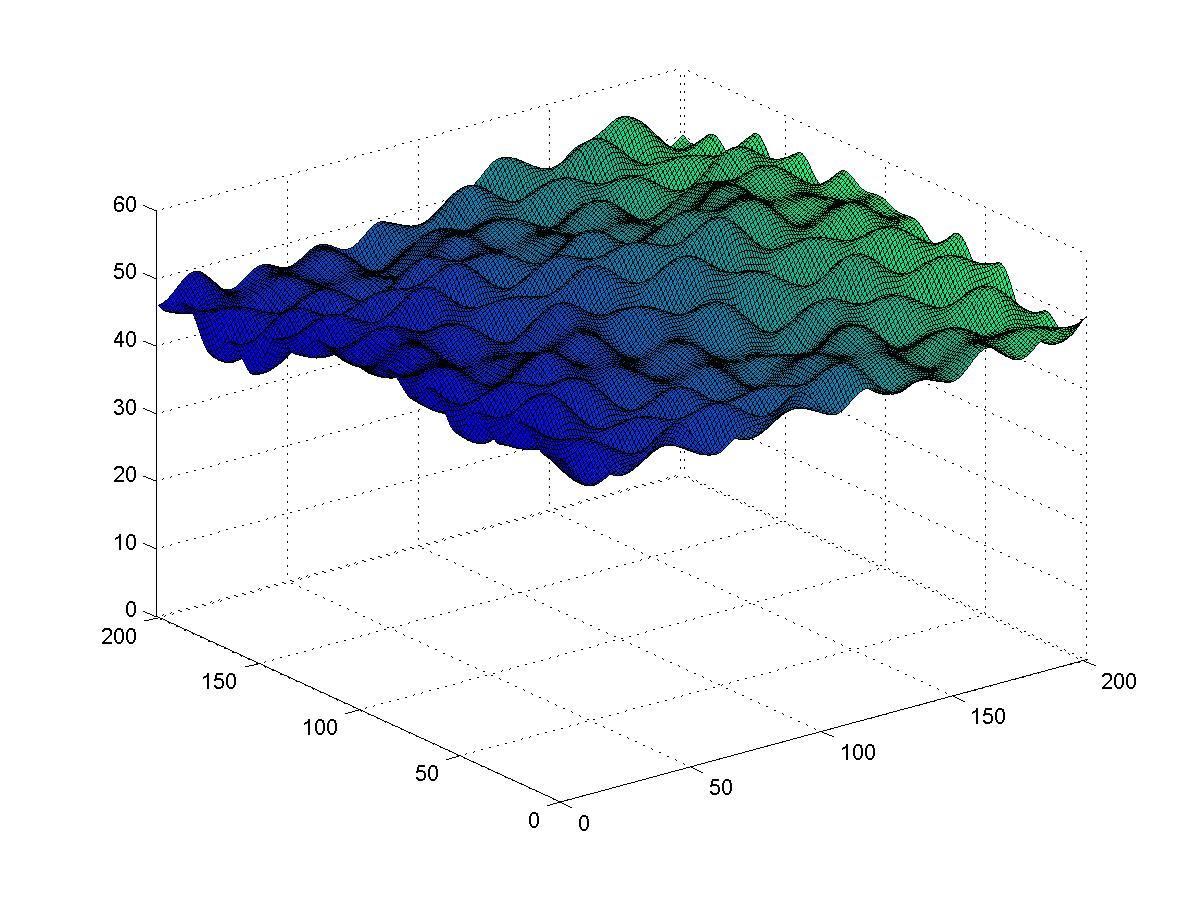
\includegraphics[width=0.8\textwidth]{fig/wavemodel}
	\caption{Simulation result of the irregular wave model}
	\label{fig:wavemodel}
\end{figure}

\paragraph{Wind model}

\subsection{Behavior of floating objects in water}

\subsection{Building simulation environment}

To test the simulation environment a basic visualization

\begin{tcolorbox}[colback=cyan!5,colframe=cyan!40!black,title=Code: Simulator.py \\ https://www.dropbox.com/s/agron9anslev6xw/Simulator.py]
\begin{minipage}{0,6\textwidth}
According to the guidelines of the seamless simulator, this part of the system has its own distinctive object. Everything related to the simulator and everything that is unknown during the mission is stored and handled here.
\end{minipage}
\begin{minipage}{0,35\textwidth}
\raggedleft

\includegraphics[width=0.8\textwidth]{img/simulatorcode}
\end{minipage}
\end{tcolorbox}

\subsection{Uncontrolled system simulation results}
\section{Control system design}


The path following control problem can be simplified to a course control problem, if the prescribed path is populated by waypoints adequately close to each other. Each waypoint is marked as visited it to ship approaches them to a certain none zero distance. Relying on these above is not always possible, therefore the controller has been extended with position-control.

\subsection{The combined control problem}

The path following problem can be traced back to an inverted pendulum system, which is a typical problem of controlling and unstable equilibrium. 

[figure, way to trace back]

The following control system has been developed for the Rudder ship type, in order to parallelize my efforts with the RobonAUT controller development, which is generally the same control problem, if the simplified system dynamics are used.

The path following problem can be traced back to a balancing problem, specifically where the ball must be kept in the center of a seesaw: [illusztrációk]
We know the dynamic behavior of the system:

$\dot{d} = g-$
$Delta_dot$

So the control problem of the boat (or car) following the path (or line) is in a narrower sense the same as leveling the seesaw with the ball in the center. [labjegyzet: in a narrower sense: this statement is only valid until the ball hits the end of the seesaw (or falls out) and the divergence of the car ($\delta$) is in $[-pi/2, pi/2]$]

A wide range of controllers has been evaluated in order to determine the best approach to solving this control system.

\subsection{Requirements of control}

\subsection{Controllers for deterministic systems}

Using the linearized state transition matrices the transfer function of the system can be formulated using:

\begin{align}
	H(s) = C*(sI - A)^{-1}B + D
\end{align}

The resulting system is a 2nd order integrator, which isn’t a surprise, if we consider the linearized output d based on the input $\Phi$. Note though, That this transfer function is valid only in a very limited range of the state variables. Due to the nonlinear system dynamics, d is periodic, unless Phi is none zero and not infinitely small.

Using this transfer function a PID steering controller can be calculated to control the system.

\begin{figure}[H]
	\centering
	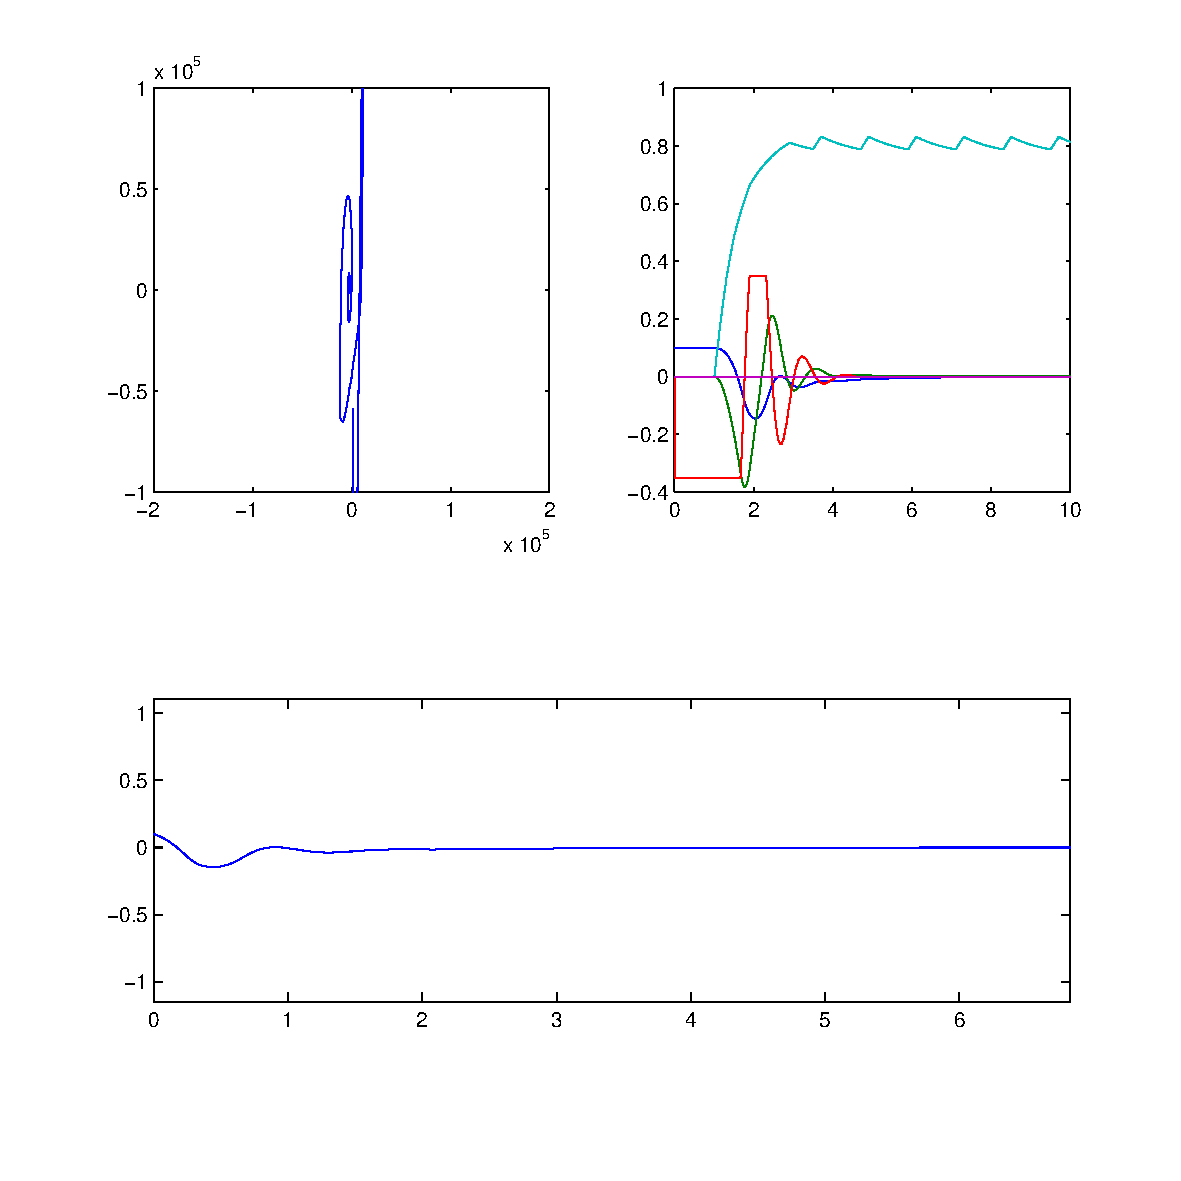
\includegraphics[width=0.8\textwidth]{img2/PI01}
	\caption{}
	\label{}
\end{figure}

The system response quality is generally low but adequate, but the serious problems arise when the system starts with larger initial conditions that are significantly different from the approximation point.

\begin{figure}[H]
	\centering
	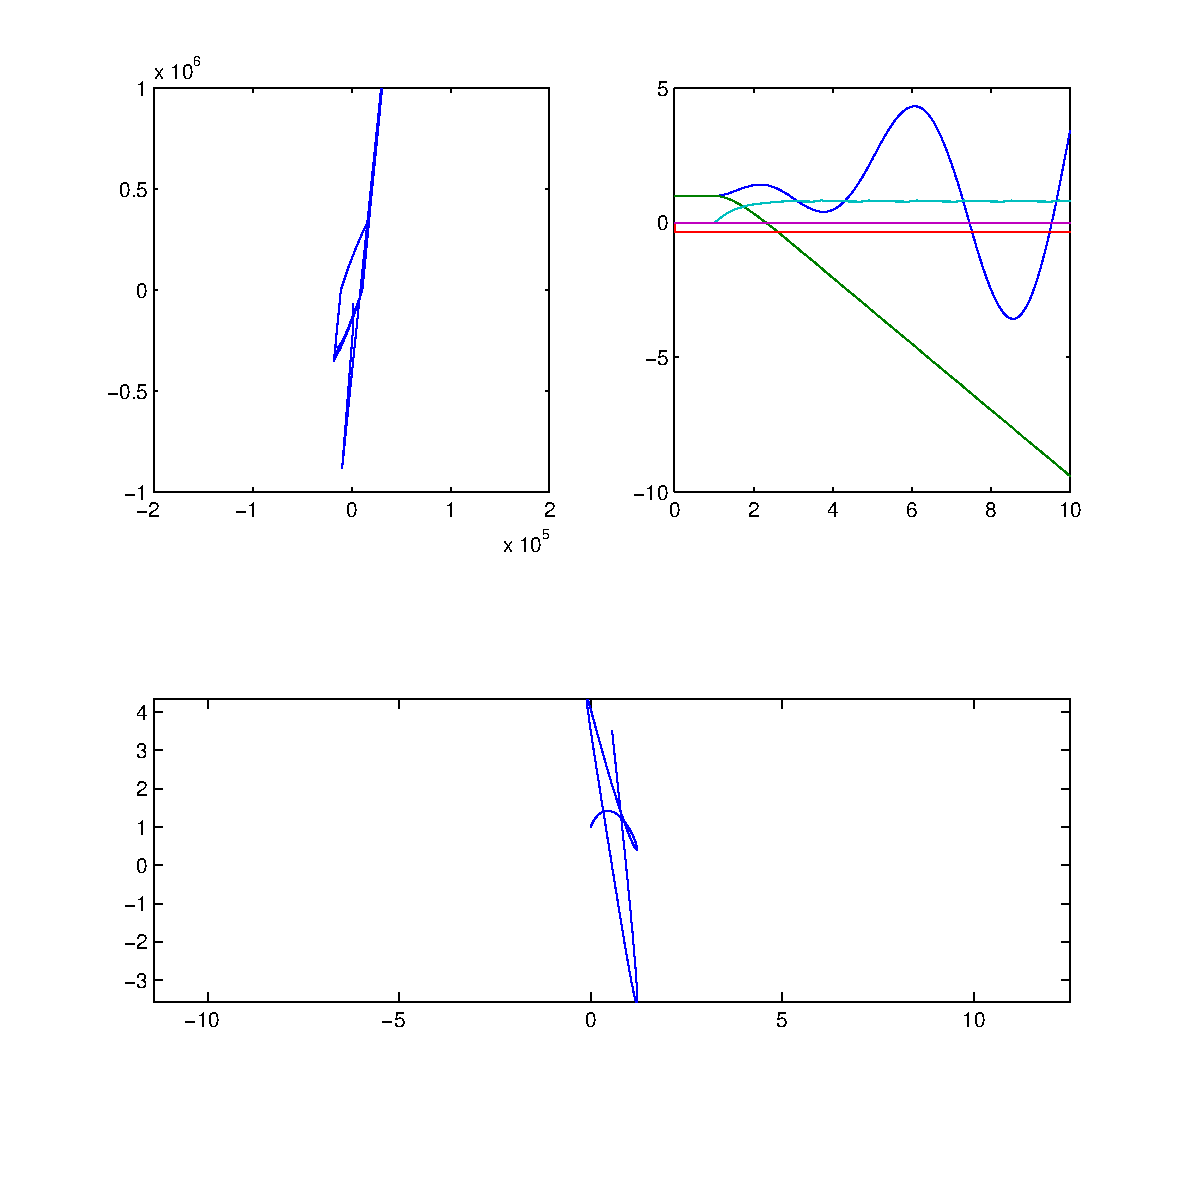
\includegraphics[width=0.8\textwidth]{img2/PI11}
	\caption{}
	\label{}
\end{figure}

The conclusion is that it’s unwise to use the pole cancelation based PID control to regulate an unstable, significantly nonlinear system. The robustness of the PID is generally low, and the system response is slow. The resulting control system is slow and unreliable.

\subsection{State-feedback controller}
In order to enhance the system response, a full state feedback controller can be computed using the same linearized system. The pole placement method allows the efficient control of unstable system, but how does it’s robustness fair against the nonlinearity of the system?

\begin{figure}[H]
	\centering
	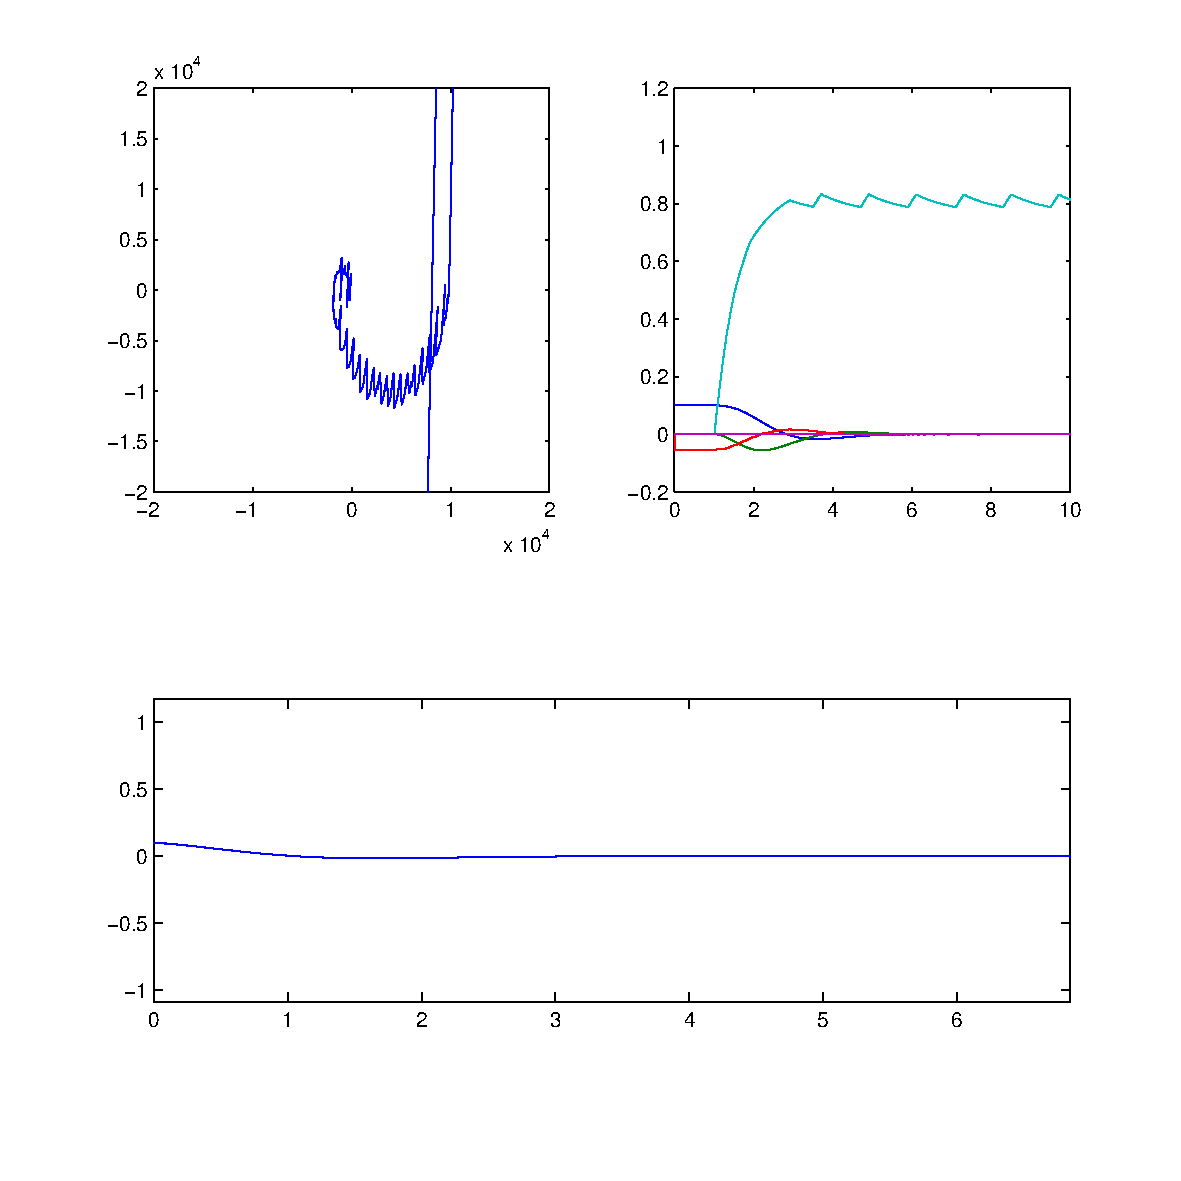
\includegraphics[width=0.8\textwidth]{img2/Lin01}
	\caption{The physical layout of the system}
	\label{fig:PhysicalLayout}
\end{figure}

The response speed is much better than the respone of the PID controller, but it contains an overshoot, which is the result of the nonlinearities. Here however the pole placement method placed the poles to imperfect locations, instead of entirely missing a pole with a zero.

\begin{figure}[H]
	\centering
	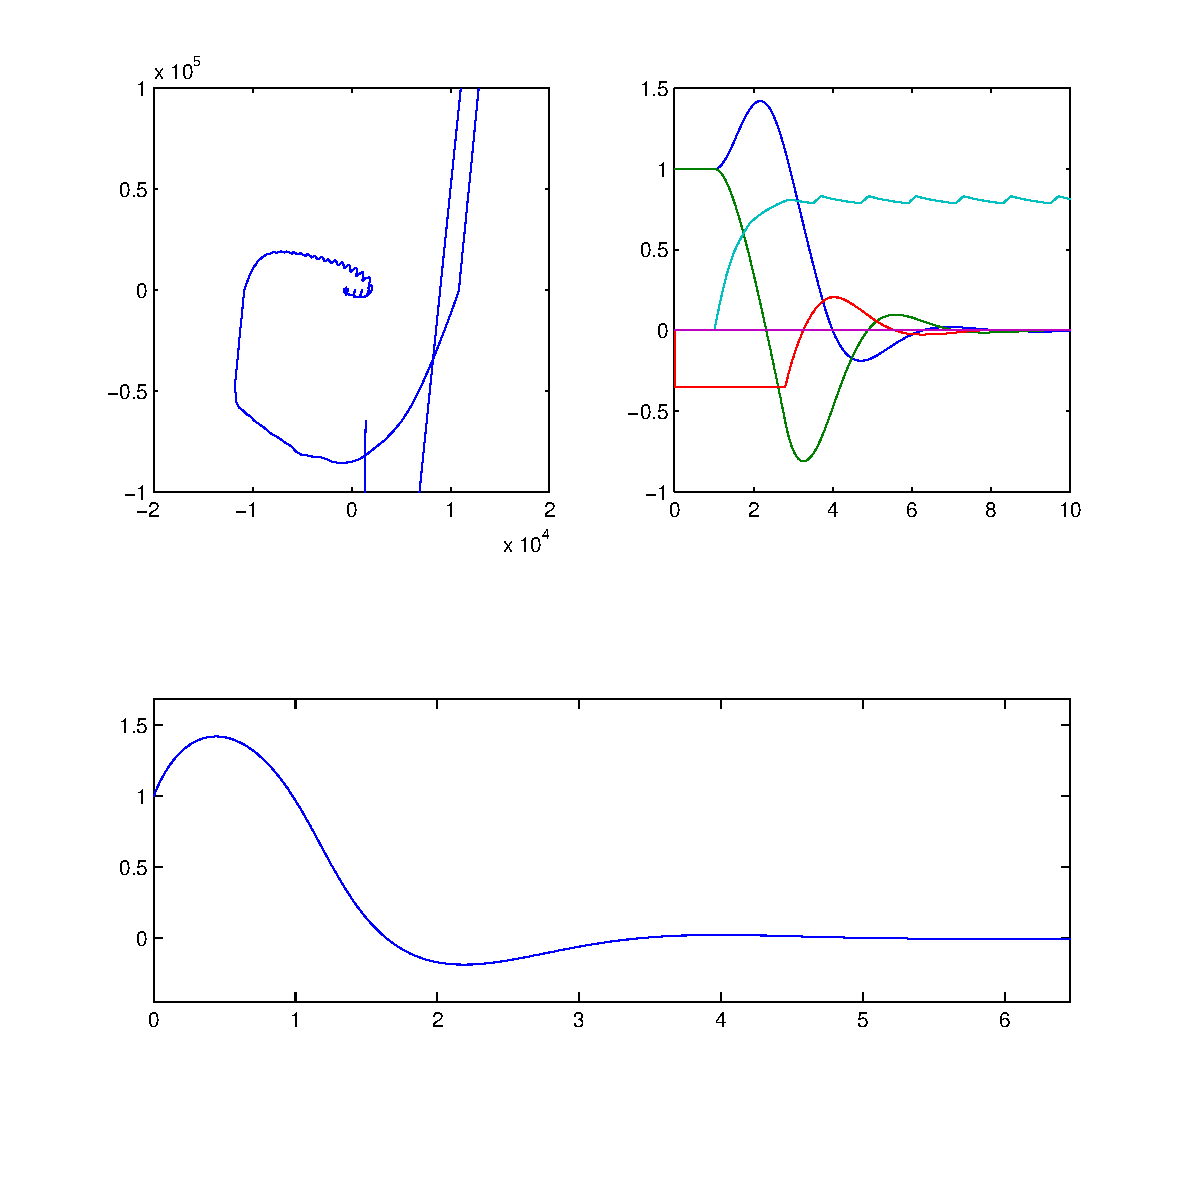
\includegraphics[width=0.8\textwidth]{img2/Lin11}
	\caption{The physical layout of the system}
	\label{fig:PhysicalLayout}
\end{figure}

As expected, the simulation result of the larger initial conditions is overshoot and oscillation, but the system will quickly settle. Of course this is not good enough yet, because the system is balancing on the edge of instability, and the effects of nonlinear sensors and measurement limitations will have additional negative effects that can cause instability.

Conclusion: the full state feedback linear controller can control the system in most cases, but is unfit to control a mission-critical system, because it has inadequate robustness and reliability.

\subsection{Hybrid switching state-feedback controller}
The instability of the linearized state-feedback controller at high Delta can be corrected by using a Hybrid controller.
the Hybrid is the bridge between linear and nonlinear control systems. The controller contains multiple state feedback controller implementations of the same system, linearized around different approximation points. The control task consists of finding the best controller for the current states, and controlling the system as a locally linear system.

For small initial conditions the Hybrid behaves exactly like a regular linear full state feedback controller.

\begin{figure}[H]
	\centering
	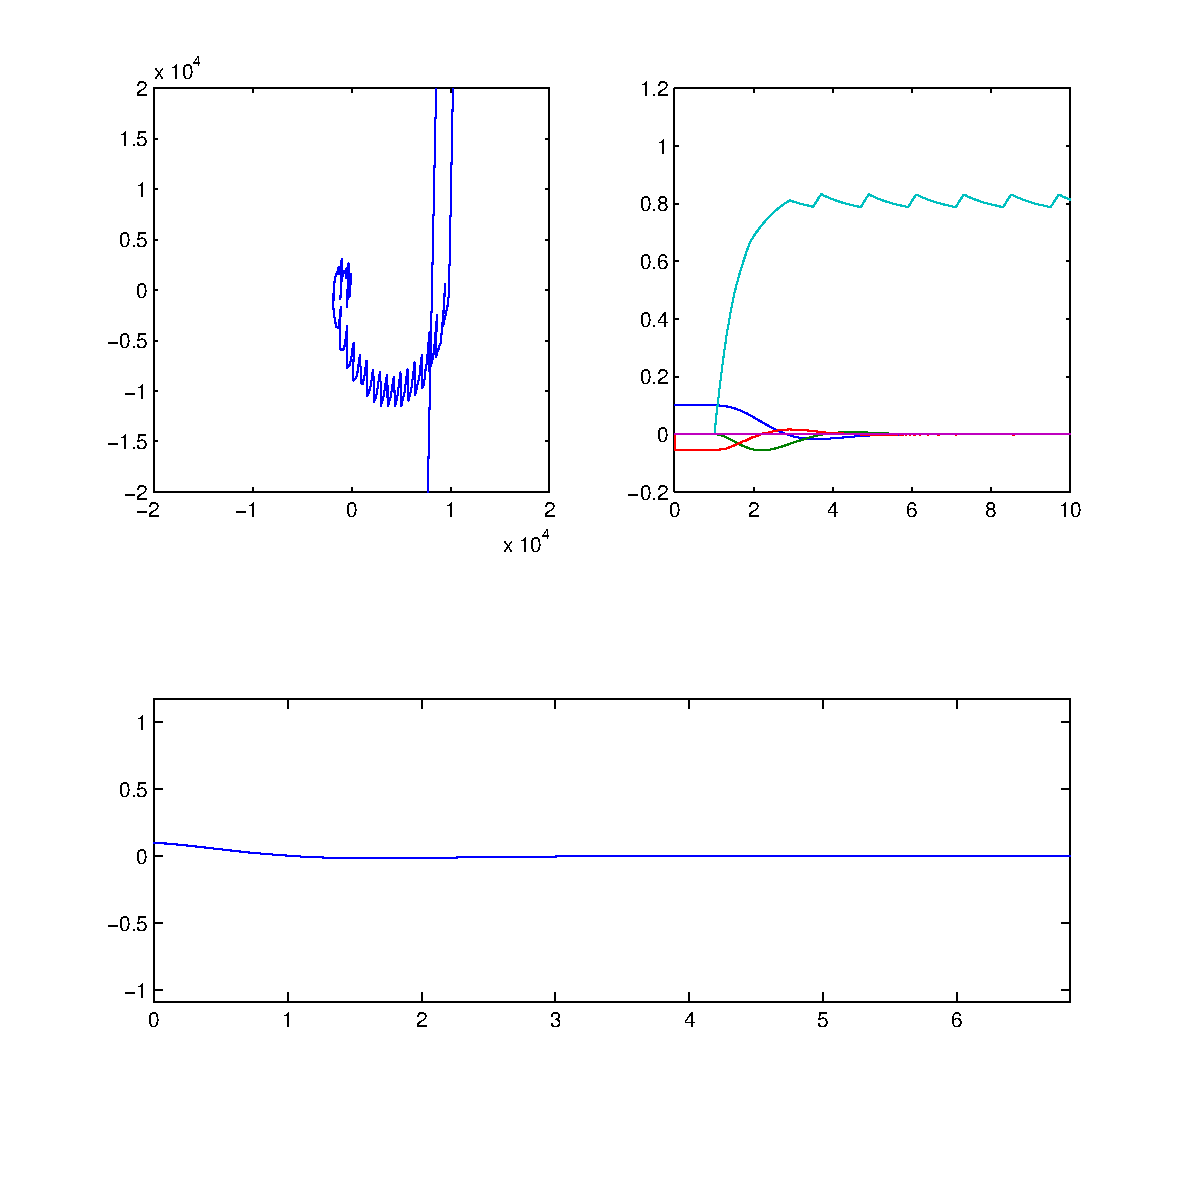
\includegraphics[width=0.8\textwidth]{img2/Hyb01}
	\caption{}
	\label{}
\end{figure}

For large initial conditions however, a different controller implementation is selected to increase the response quality. In this case however the system reaction involves only small nonlinearities, therefore a slight decrease in settling time can be observed, but nothing major. As the $\Phi_{max}$ is increased, so does the nonlinearity of the control signal, and the more the response quality is increased by the hybrid controller compared to the linear.

\begin{figure}[H]
	\centering
	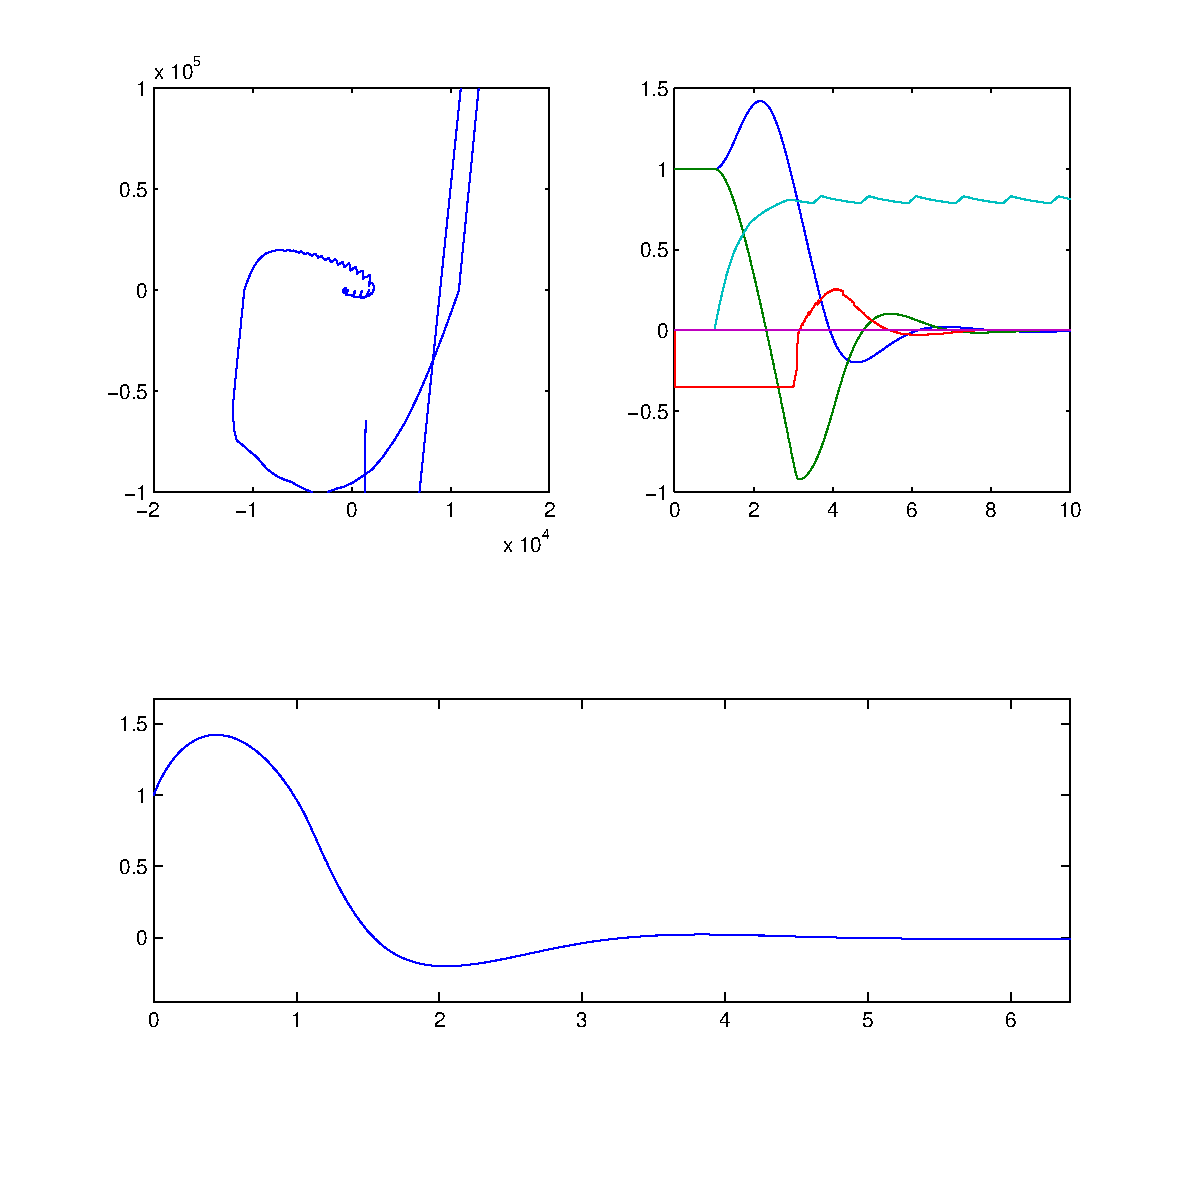
\includegraphics[width=0.8\textwidth]{img2/Hyb11}
	\caption{}
	\label{}
\end{figure}

The Hybrid controller has serious dangers and disadvantages however. If the control switching is not implemented correctly, it is possible to destabilize a stable system, and trigger the divergence of the states.
Additional disadvantages include the unwanted and unpredictable system responses if a controller switch occurs. This problem can be reduced by controlling the change of the control signal, instead changing the control signal directly, therefore the jumps in the control signal can be eliminated.
Another disadvantage is the possible necessity of having a large number of controller implementations. For example, linearizing around 3 state variables with a definition of 10 linearizations each results in 1000 separate controller implementations.

If having a large number of control implementations is not a problem, the process can be automated using the symbolic toolbox of MATLAB (or any other similar software) if the correct nonlinear state-transition functions are know.
The symbolic toolbox allows the automated formulation of the Jacobi matrices and the software can compute the linearized implementations cyclikally, then store them in a lookup table. 

\subsection{Fuzzy controller}
Though linearizing around many approximation points can result in a relatively smooth switching experience, the number of required controllers can quickly become unreasonably high. The fuzzy controllers address these problems and provide a solution for smooth switching and low number of controllers. Additional advantage of the fuzzy controller is the Fuzzy Control Language, which is the de-facto standard Domain Specific Language for developing fuzzy logic and controllers. The use of FCL helps to understand and design the switching methods which is an important part of the Hybrid controller design.

The Fuzzy controller has an important property that differenciates it from the rest of the controllers evaluated here: the formulation of the control system is based on “liquid” facts, instead of solid data. This results in a less-optimal control, but can ensure stability for systems with unknown dynamics. The fuzzy controller is expected to produce a system response of lesser quality, however it’ll have an important role in controlling the more complex, only partially known ship dynamics presented earlier.

Unfortunately there was no time to finish the testing of the Fuzzy controller, therefore the results will be included in a later version of the document. 

\subsection{State Ordinance Controller}
The system response can be enhanced further using unconventional controllers. This “State Ordinance Controller” (OC) couldn’t be any more unconventional, because it’s the result of my early ignorant implementation of a sliding mode controller, but it can provide surprisingly good system responses and boasts a very simple mathematical background and implementation.

The essence of the OC is to determine a priority order of state variables and control the individual states separately by specifying spaces and surfaces. By forcing the state variables into the spaces and onto the surfaces, arbitrary system response can be achieved (of course the physical limitations apply here as well).

The example system is the steering control of the car. The divergence ($\delta$) is forced onto a surface function of distance (d) by controlling $\Phi$. If $\Phi$ is controlled correctly, $\delta$ will stay on the surface. If the surface has been defined in a way that if $\delta$ is on the surface then
$$
\dot{d} = f(x)
$$
function is negative-definite, then d and $\delta$ will approach zero together.

[figure]

Considering the nonlinearities of the system

$$
max(|\dot{d}|) = v
$$

if $\delta = +-pi/2$. This generates the highest-priority natural space for $\delta$.

So $\delta$ is forced to onto the following final function:

[figure]

So a basic implementation of the control system could be:

\begin{align}
	\Phi = sgn(sat(d,[-\frac{\pi}{2};\frac{\pi}{2}]) - \delta) * \Phi_{max}
\end{align}

Of course the controller response would be a high-frequency switching of $\Phi$, resulting in Zeno's paradoxes, which is undesireable. So instead of the signum function another saturation function can be used with values between -1 and 1, with an additional permissible error ($\varepsilon$) parameter. The higher the permissible error, the lower the frequency of the chattering will become.

\begin{align}
	\Phi = \frac{sat(sat(d,[-\frac{\pi}{2}; \frac{\pi}{2}]) - \delta, [-1; 1])}{\varepsilon} * \Phi_{max}
\end{align}

Re resulting system response:

\begin{figure}[H]
	\centering
	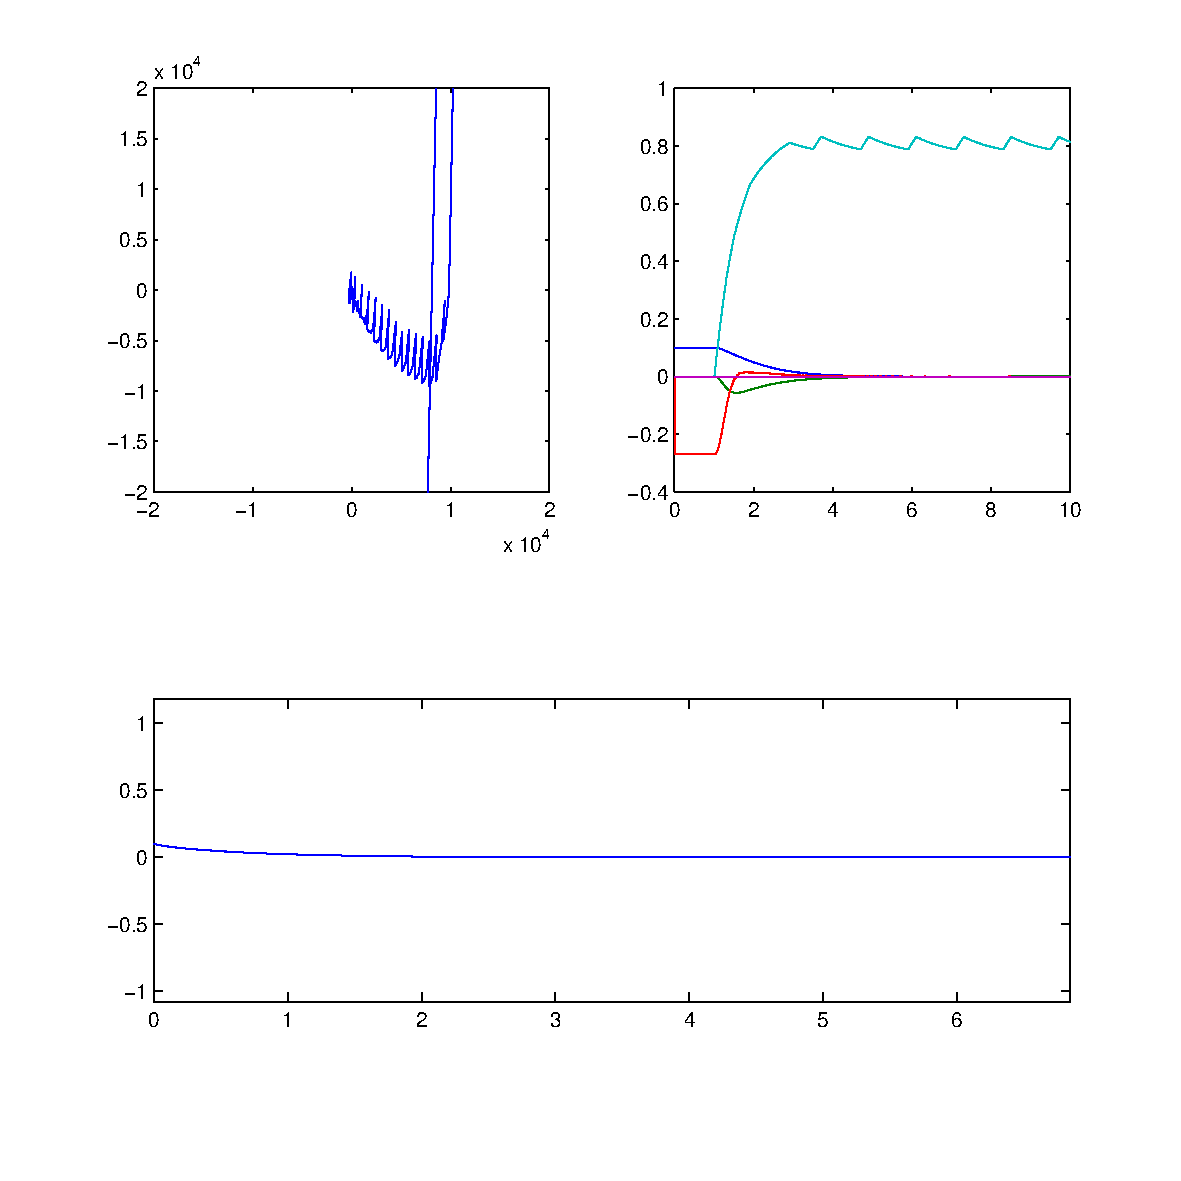
\includegraphics[width=0.8\textwidth]{img2/Ord01}
	\caption{}
	\label{}
\end{figure}

And the resulting system response fir large initial conditions:

\begin{figure}[H]
	\centering
	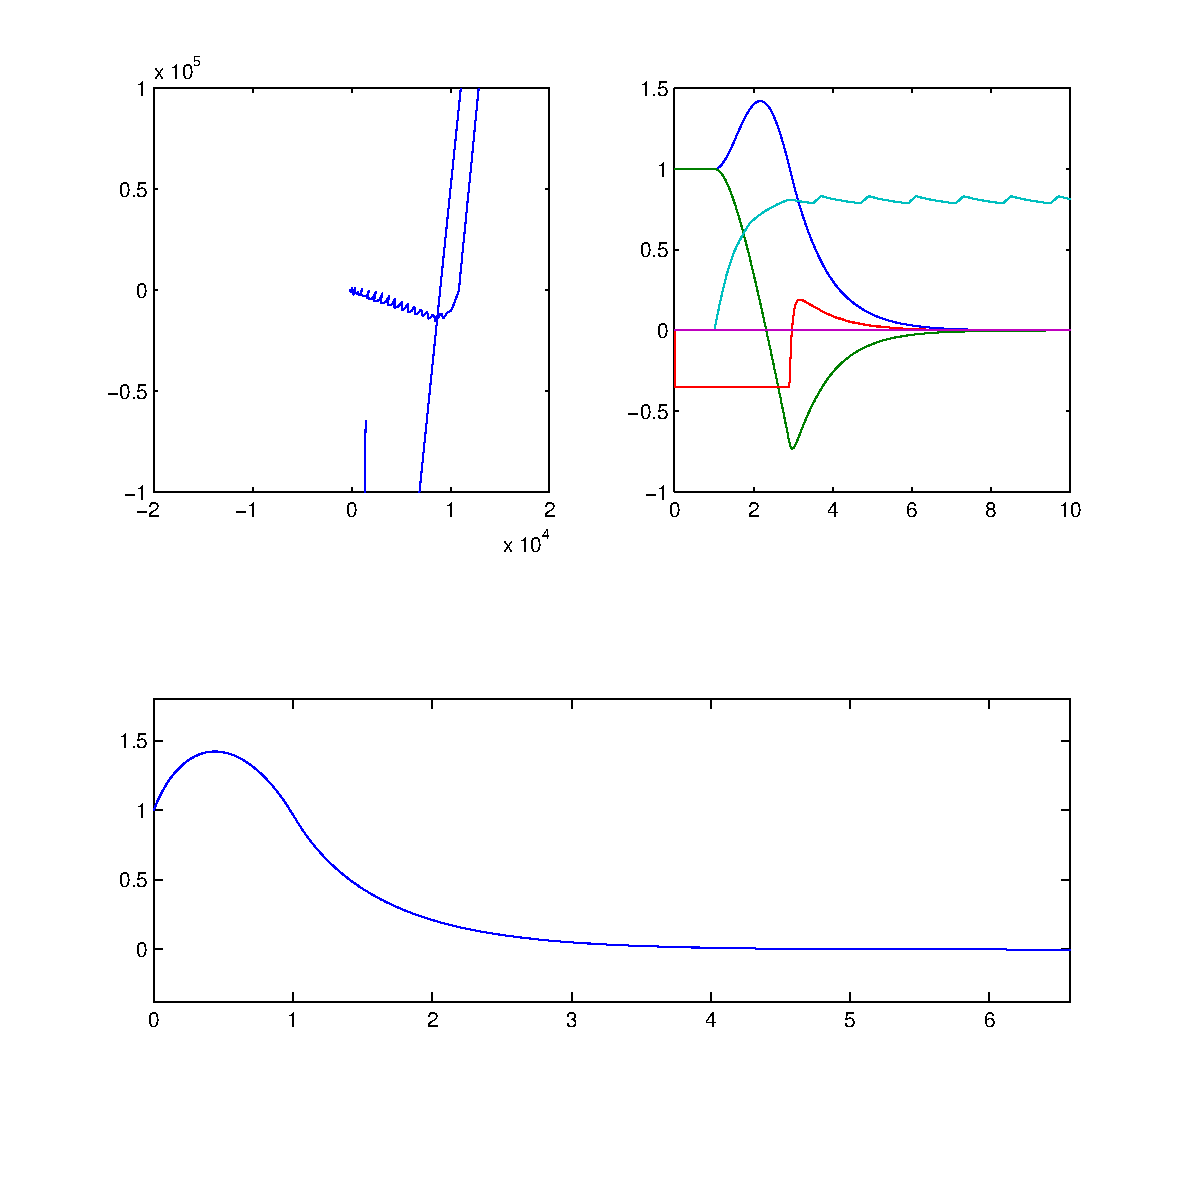
\includegraphics[width=0.8\textwidth]{img2/Ord11}
	\caption{}
	\label{}
\end{figure}

By changing the natural space of $\delta$, different trajectories can be achieved, like a shallower approach to the path:

[figure][figure]

Additional spaces or surfaces can be introduced, like the limitation of $\Phi$ based on the speed and the limitation of the acceleration based on $\Phi$ for a basic traction control.

The resulting control system excels in robustness and system response speed, but the order of prioritizing the state variables requires some intuition (general rules of thumb can be applied however).
The downsides are the virtually nonexistent documentation (excluding this document) and lack of mathematical background (yet).

The result is a robust and fast controller for any initial conditions and some system inaccuracies, and can be considered reliable because the controller can be formulated directly to the nonlinear system.

I consider this type of controller the bridge between fuzzy control and the Sliding Mode Controller.

\subsection{Sliding Mode Controller}

The Sliding Mode Controller is an ambivalent control method. It’s a very powerful tool to directly control nonlinear systems, but the formulation can be tricky.

“The common Lyapunov function is an elusive beast that you can almost never find.” [Magnus Egerstedt, Associate Chair for Research and External Affairs, Georgia Institute of Technology]

The central concept of the Sliding Mode Controller is to combine the deviations of the state variables from the reference input and unite them in the combined error function. Then use the Lyapunov function of the dynamical system to prove that there exists a controller that the trajectory of the combined error will hit a surface, starting from every possible initial condition, and then it will move along the surface to reach zero.

In practice a Lyapunov candidate function can be determined, then design the controller based on the combined error function.
Formal proving that such a controller exists is very hard, but in the current control case general considerations can lead to the same conclusion: it does. If $\Phi ~= 0$ then the system is stable (not asymptotically stable, but stable). Therefore a sliding surface can be determined for the combined error function.

The system response is quick and lacks the overshoot

\begin{figure}[H]
	\centering
	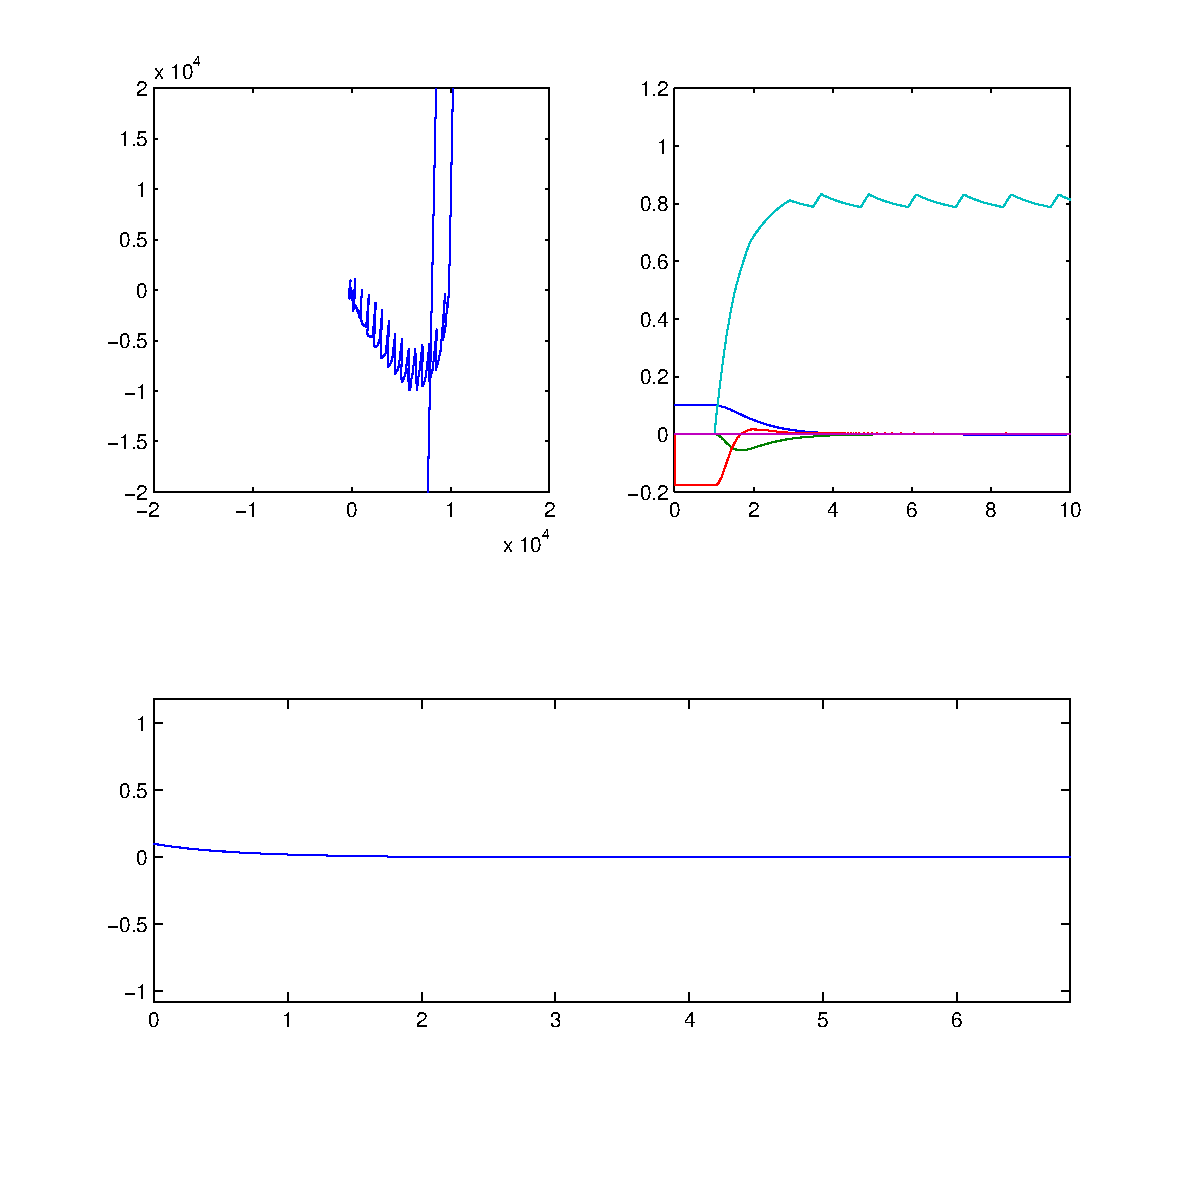
\includegraphics[width=0.8\textwidth]{img2/Sli01}
	\caption{The physical layout of the system}
	\label{fig:PhysicalLayout}
\end{figure}

And very reliable for larger initial conditions as well.

\begin{figure}[H]
	\centering
	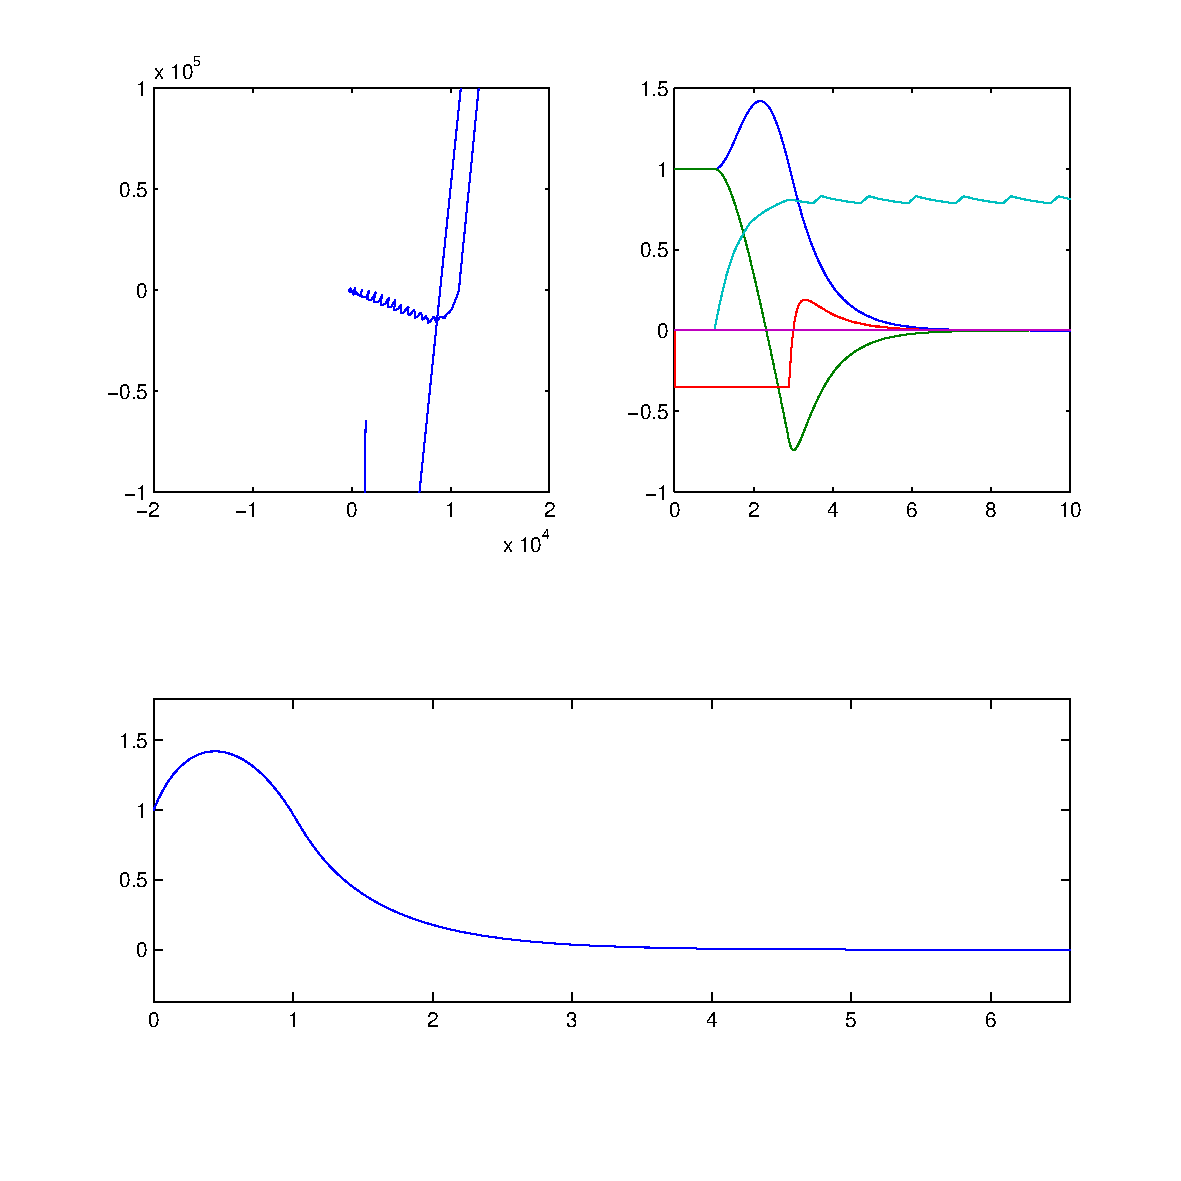
\includegraphics[width=0.8\textwidth]{img2/Sli11}
	\caption{The physical layout of the system}
	\label{fig:PhysicalLayout}
\end{figure}

\subsection{Model predictive control}

The model predictive control was not evaluated, because the control problem at hand allows quick data acquisition and has virtually zero time-delays. The real strength of model-based control is to predict the states and outputs of a complex system based on numerous inputs, if relatively large time delays are present. The model-based control is ineffective at small scale operations, because it’s very CPU-heavy, and it’s prediction capabilities are useless with a fast system responses.

Alas, a precise model of a large scale ship includes several underlying states with delayed effects, thus calling for a model predictive control, because a single tiny overshoot in the orientation control of a container-transport can be measured in kilograms of fuel.

\subsection{Comparsion of results}

The evaluation results of the controller types are depicted in the following diagram:

\begin{figure}[H]
	\centering
	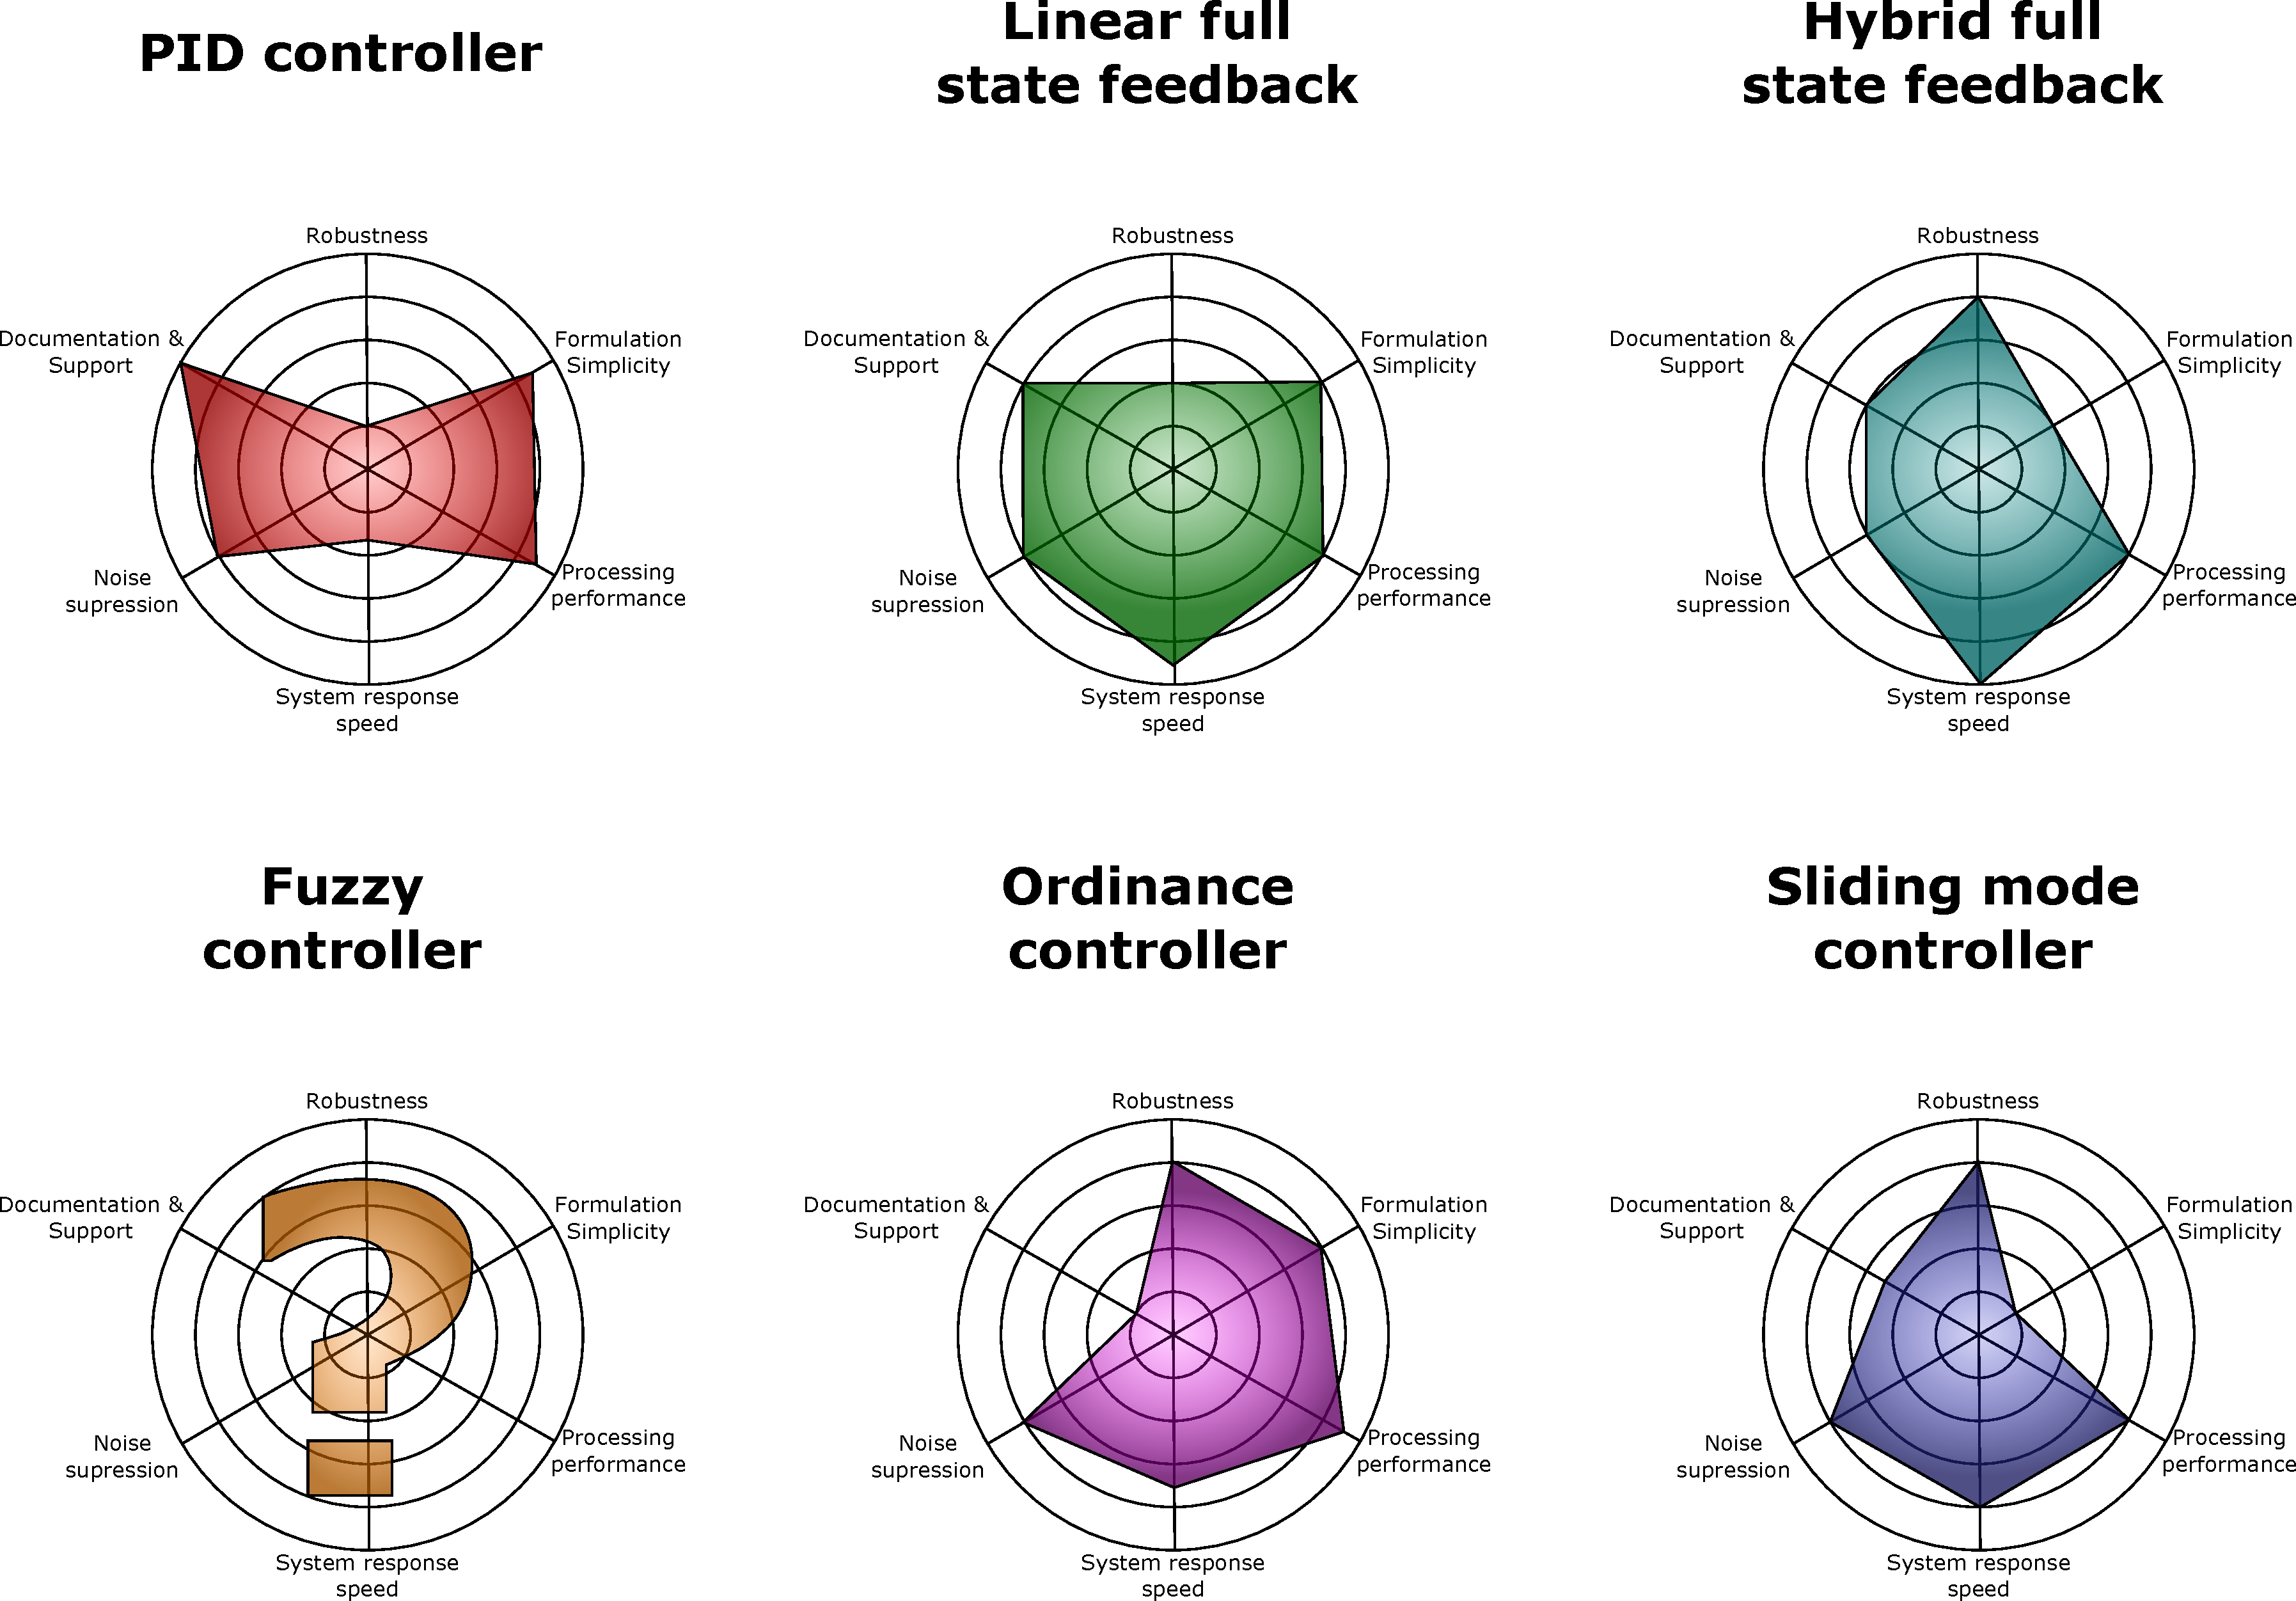
\includegraphics[width=1\textwidth]{img2/ControlCompare}
	\caption{The physical layout of the system}
	\label{fig:PhysicalLayout}
\end{figure}

Final results can’t be concluded yet, because the evaluation of the Fuzzy controller is missing, and the final system is expected to be much more complex than the current test system. Also extensive research must be made to determine the robustness against noise and limited measurements and outputs.

However, the linear full state feedback controller has proven itself to be superior to the other evaluated control systems, because of it’s simple formulation and quality system respone. However, the reliability of the Linear state-feedback controller quickly decreases as the system nonlinearities and uncertanties increase.
In that case the use of a sliding mode controller or ordinance controller is justified, depending on the complexity of the system. The ordinance controller might provide quick and effective results, but if an unambiguous priority can’t be established, then the formulation of a comprehensive sliding mode controller is necessary.
\section{Logical system}

This section will give a preliminary overview about the logical and physical layout of the system. The design steps were implemented using the guidelines of the Model Based Design approach, therefore the the logical layout resembles the physical. However, for a lighter approach, the layouts will be introduced separately and connected later.

\subsection{Concept of separation}

This basic layout describes the logical connections of the system:

\begin{figure}[H]
	\centering
	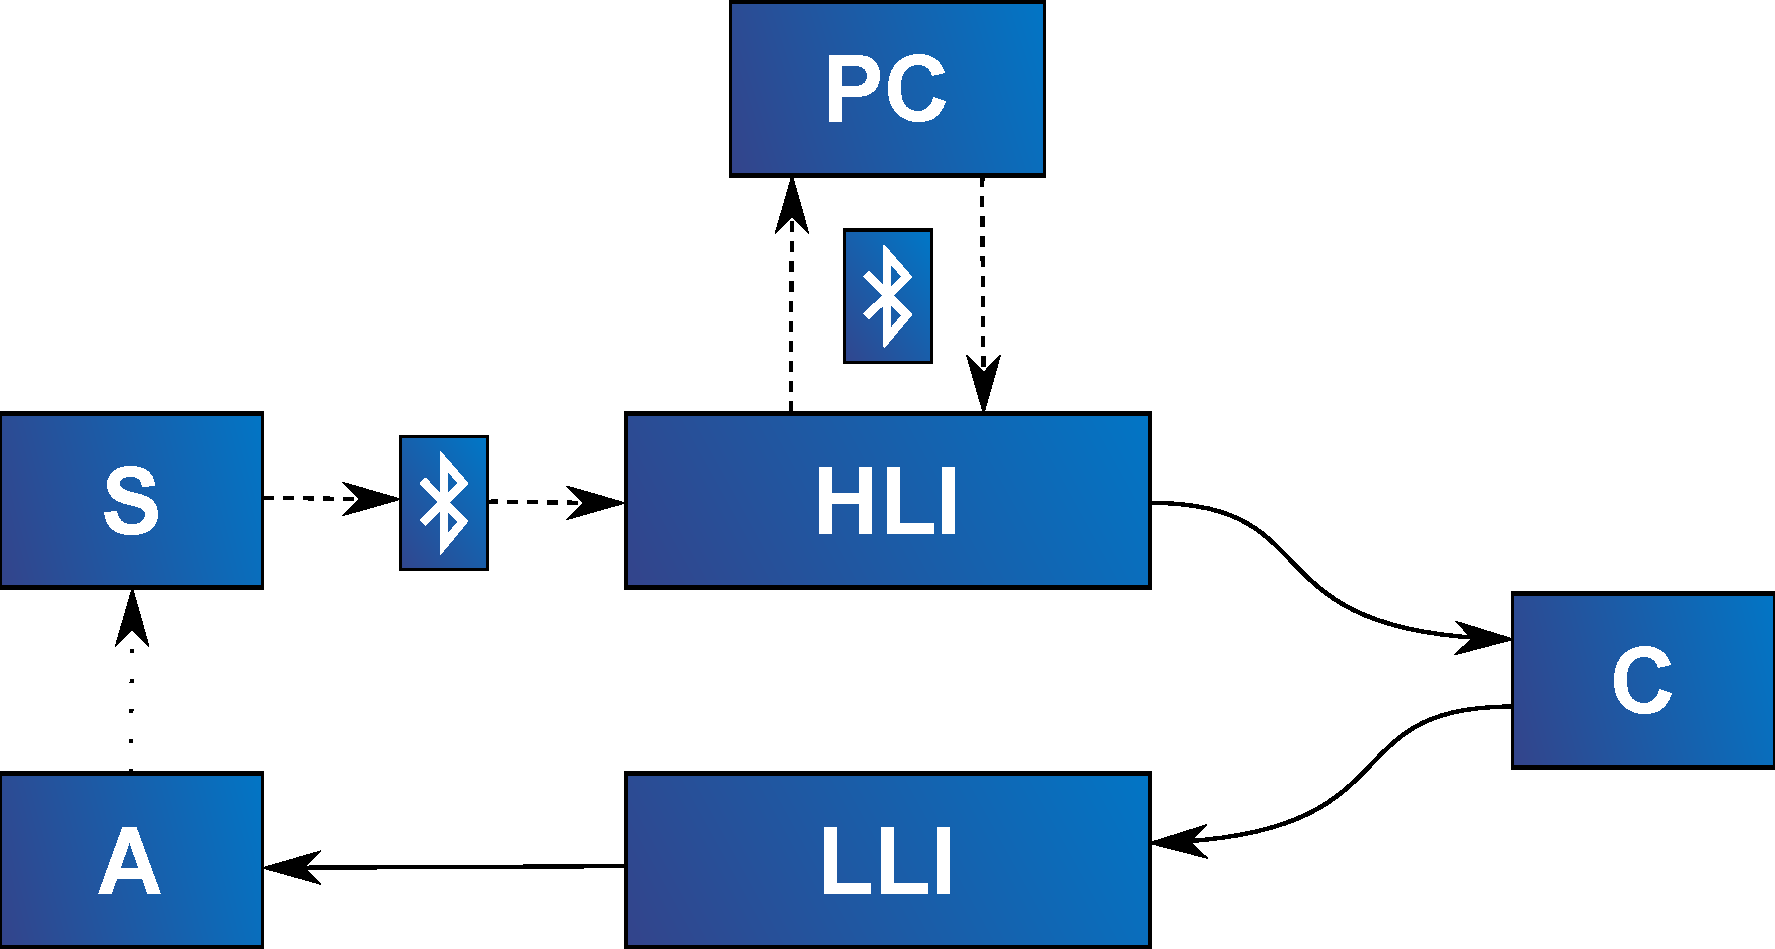
\includegraphics[width=0.8\textwidth]{img2/LogicalLayout}
	\caption{The logical layout of the system}
	\label{fig:LogicalLayout}
\end{figure}

The High Level Interface (HLI) processes the position and orientation sensor data input from Bluetooth serial port. During regular navigation the HLI applies the filtering to the inputs, then outputs the estimated orientation divergence from the path, and the estimated distance from the path. The Controller (C) processes this data and returns the required inputs to the system. The LLI processes this physical signal and transforms them to PWM signals, then applies it to the power electronics and the Actuators (A), which will have the final effect on the system.

It’s important to note in this diagram, that the Controller and is separated from the rest of the software. This enables the user to radically modify the configuration of the robot, or try multiple controller implementations and switch between them real-time. The 
Such a switching system can handle possibly expected failures and breakdowns up to a certain level (like the malfunction of one of the engines of a twin-propeller aircraft).

\section{System design}

\subsection{Physical layout}

The more detailed physical layout diagram shows the actual relations of the modules of the system to each other. There are several rapid prototyping technologies working together, all of them based on very high level languages.

The embedded system is running Angström Linux, which is a lightweight linux distribution. It enabled the use of Python and USB Hardware-extensions, a generic cheap USB Bluetooth Dongle and a webcam (The webcam is working, but it’s not supported yet on the software level).
Using Linux as the operating system of the embedded device has the additional advantage of manually controlling and updating the system through SSH.

The HLI and LLI are both implemented in Python. They communicate through function calls implemented via Cython. The actual Controller and Kalman Filter run natively, the .c/.h source code is compiled to .so files by the Cython compiler, which can be imported into the main python software as a static function library.

The source code files are generated by MATLAB Embedded Coder, based on the Simulink model of the control system. The resulting functions are more like objects, containing inner states and member functions, but only one instance can exist of the same controller object.

The GPIOs are controlled from Python as well, using system calls.

\begin{figure}[H]
	\centering
	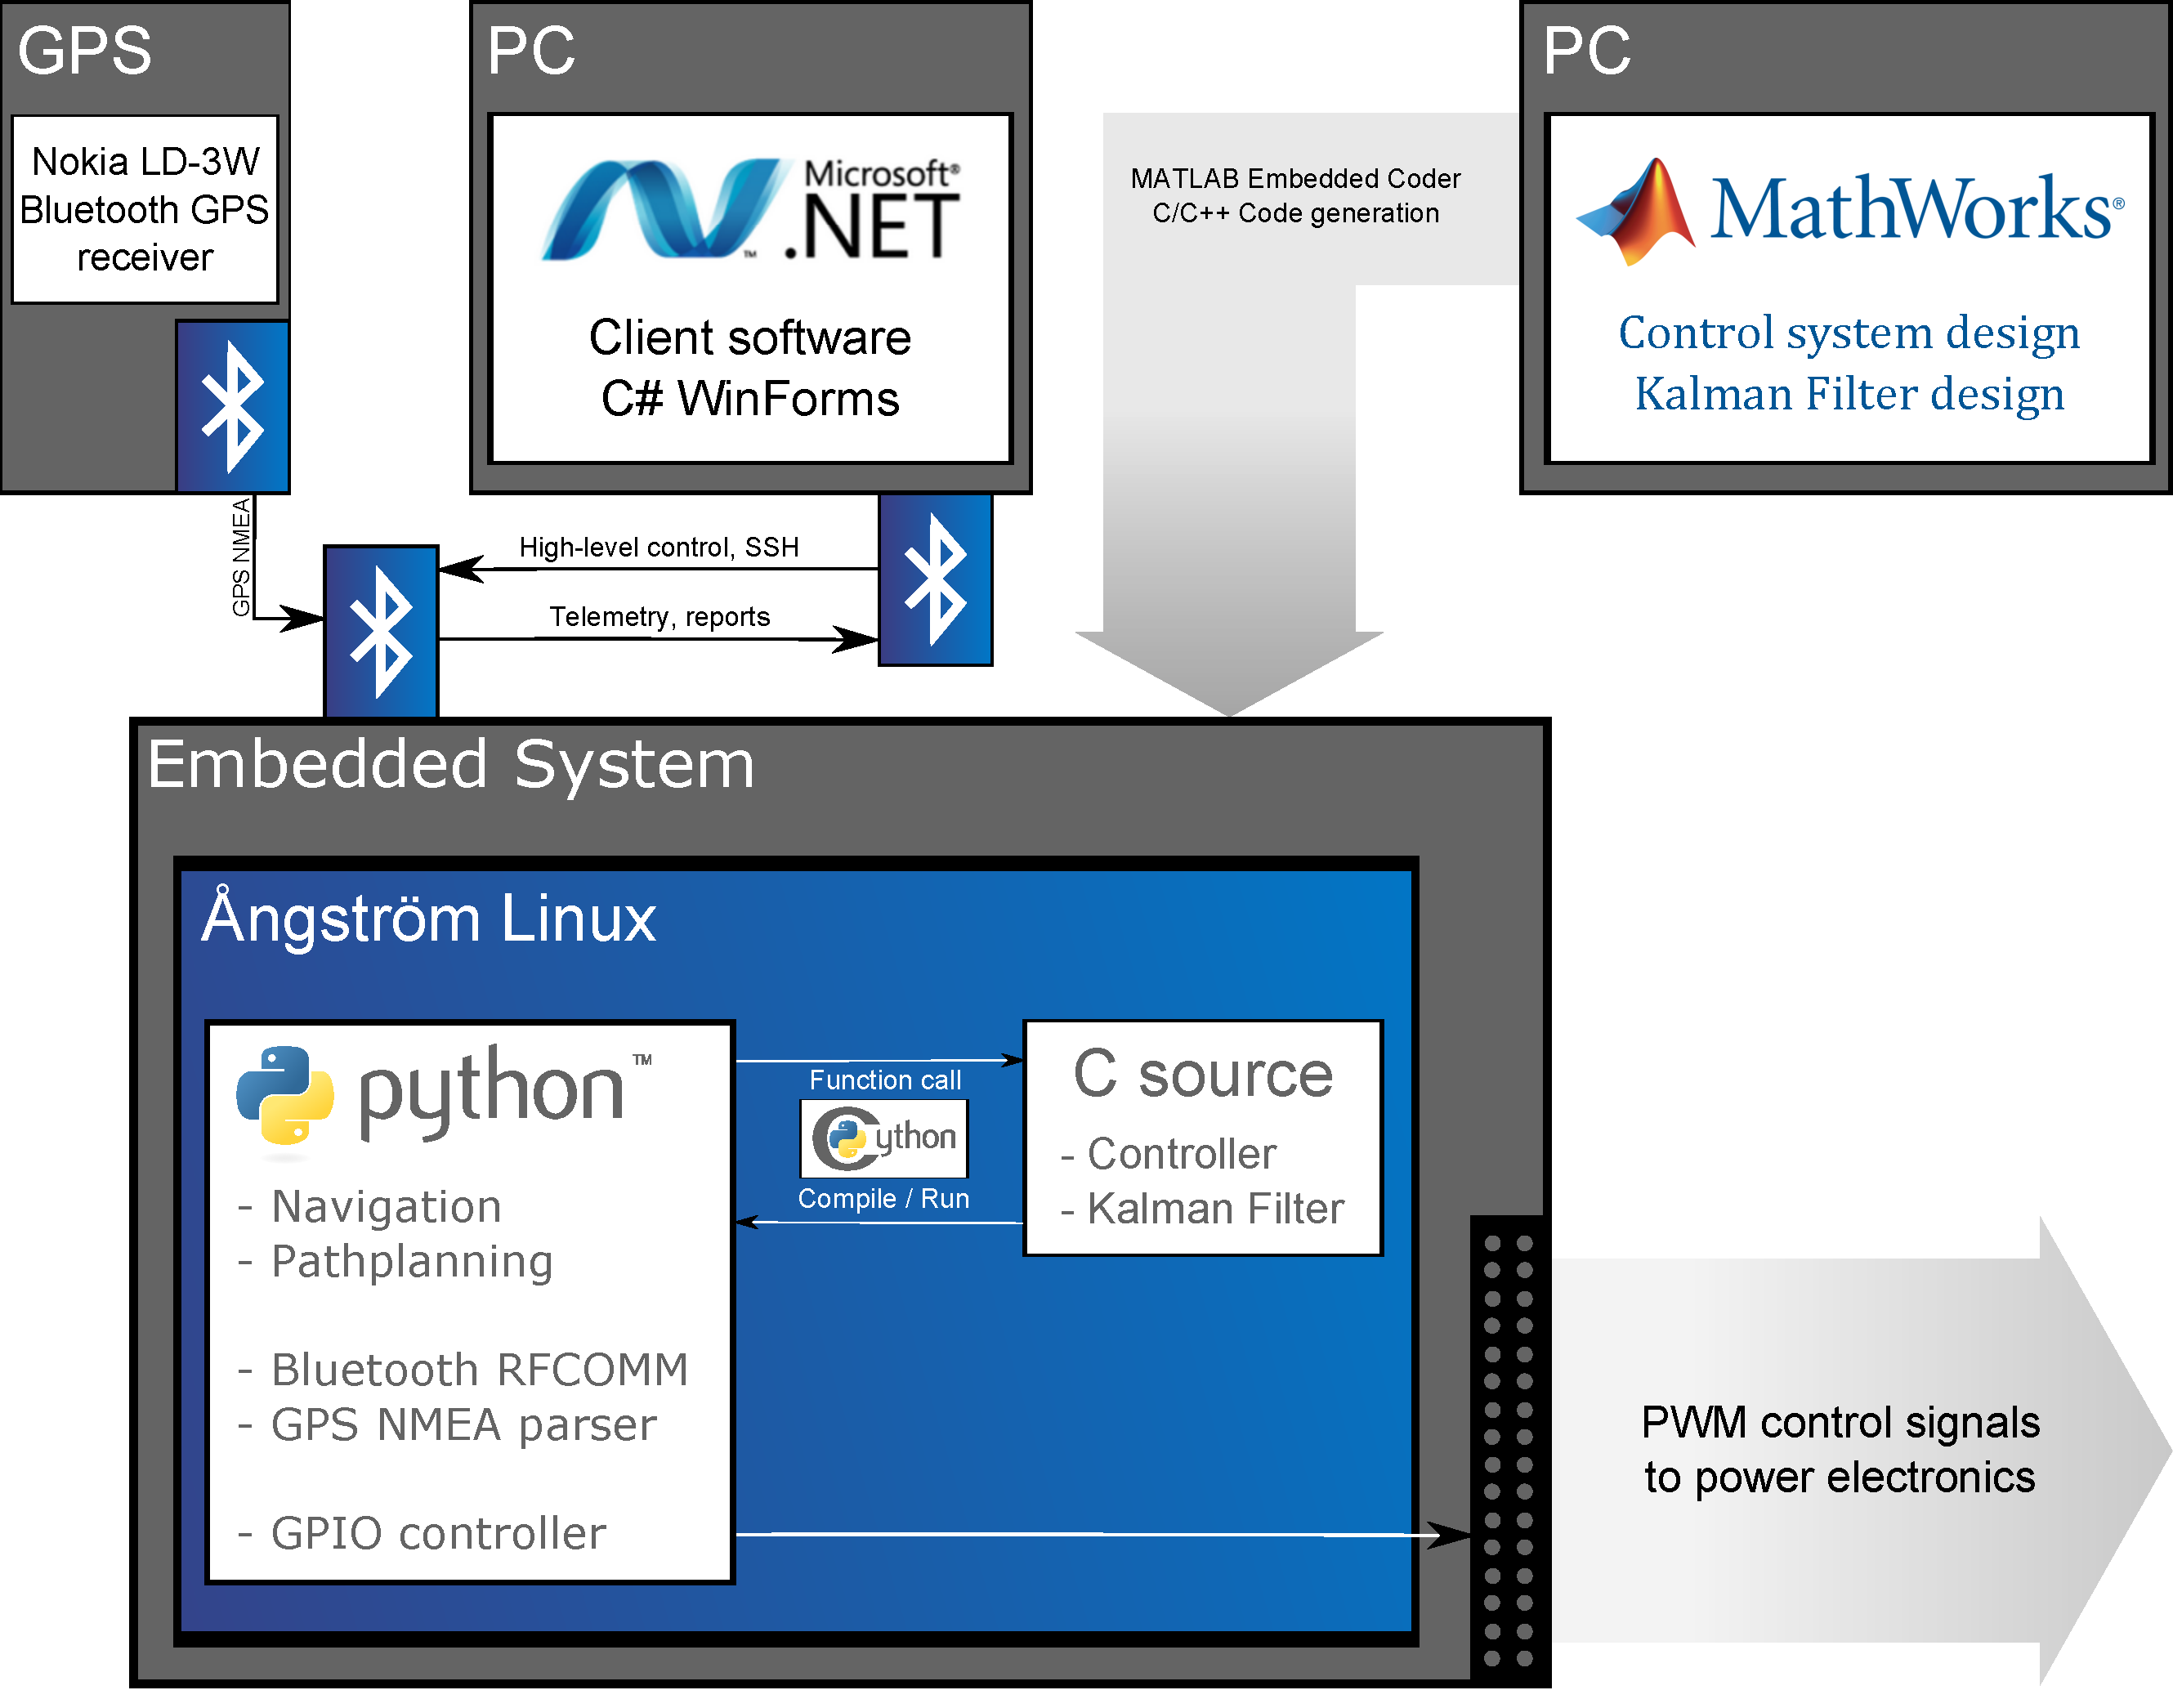
\includegraphics[width=1\textwidth]{img2/PhysicalLayout}
	\caption{The physical layout of the system}
	\label{fig:PhysicalLayout}
\end{figure}

The Embedded system has an USB Bluetooth hardware extension that communicates with the GPS receiver and the Client software.
It’s important to note, that the GPS receiver and the Embedded system are physically close to each other (relative to the scale of the ship), always within the range of the Bluetooth connection. Using wireless communication however enables the distant placement (relative to the scale of the circuit board) in order to ensure high GPS reception and a protected environment for the embedded system as well (e.g.: top of the mast and the belly of the boat).

\subsection{GPS Acquisition}

The localization procedure is implemented by a GPS (Global Positioning System) receiver, connected to the BBB via Bluetooth. The actual device is a Nokia LD-3W GPS device produced for Bluetooth-enabled smartphones without GPS connectivity. The receiver includes a battery with a relatively long life. Solar charging of the device is possible. [wrapfigure]
The Nokia LD-3W transforms the GPS signals to NMEA sentences that can be parsed to extract the current position, speed and much else.

\subsection{Bluetooth connectivity}

\subsection{Sensors and effectors}
\section{Hardware design}

\subsection{Remote control}

\subsection{Hardware}

\subsection{Assembly}
\section{Path planning} 

Marine navigation seems very simple and starightforward at the first glance, one might want to ask what's the reason to put serious effort into a pathplanning algorithm, if ships can sail in straight paths? Although this is a fair point, the maneuvering of ships is rarely restricted to open seas, without any obsticles to avoid, and even then sailing vessels require active planning, as they rarely move paralell to the wind direction, or other disturbances may apply, like ocean currents.

The problems of navigation and pathplanning will be introduced gradually. There are two kinds of boats (bowerboats and sailing), two types of environments (still water and riverine) and two areas of applications (shortest route between points or shortest traversal of an area). In summary there are eight problems to be solved, each getting more complex than the one before. Fortunately, it's enough to solve only some key problems, then combine the findings to a roboust pathplanner.

\subsection{Model of maps and obstacles}

The forms of obstacles in the sea can vary between wide levels of complexity. The operation space can be either be completely open, or closed.
[img of ship in open vast space and satellite image of Balaton]

They might contain very simple or very complex inner structures.
[satellite img of svalbard]

Or the free space can be just a strait or as narrow as a river. In the latter case especially, the local traffic of other vehicles must never be ignored, or accidents might occur.
[img of crowded bosphorus, sailboat in the danube]

/subsection{Global Path planning}

Several algorithms have been developed for global path planning, and this field of study is still researched extensively. The different methods result in very different paths, some of them are optimal, others are not, and some algorithms might even fail to create a path at all. Their performance varies greatly by the different environments they are executed in. A complete overview of all possible motion planning strategies is not in the scope of this document. Some that might be fast, reliable and optimal in certain areas might fail completely in others. In order to find the best navigation solution for each environment, the following algorithms will be analysed and compared to each other in different settings.

\paragraph{Cell decomposition}

Cell decomposition methods are the most used and researched path planning field in outdoor robotics /cite[pathplanning_overview]. The region is broken down into discrete, non-overlapping fields. the union of these fields is the original region. The method has three sub-categories, the Approximate, Adaptive and Exact Cell Decomposition. We will only discuss the Approximate method.

The most widespread of all Cell Decomposition algorithms is the A* search. It lays a grid down over the area to obtain the cell points, representing a graph. Then a best-first search is used to determine the least-cost path between the starting point and the goal. While traversing the graph, A* follows the path of lowest expected total cost. It keeps a sorted priority queue of the cells that need to be examined.

The order of the nodes to be visited are determined based on a cost function based on the past path-cost and the future-cost estimated by heuristics.

[image collage showing how A* works in different environments]

\paragraph{Roadmap}

Roadmap methods use sparse graphs to represent the connectivity between free spaces. The most commonly known algorithms in this group are the visibility graph, or Voronoi-diagram based. Although they have common basics and restrictions, they are significantly different. The former produces an optimal, but unsafe path, as it passes very close to the vertices of the obstacles, the latter generates a rather safe, but suboptimal path, because it aims to keep maximum distance from surrounding objects.

[visibility graph and voronoi diagram comparison]

But the most important is, that we will use neither of them. They require a special polygonal obstacle model, and 

\paragraph{Wavefront}

\paragraph{Comparison of algorithms}

[comparison of path length, execution time, execution efficiency (path length / execution time) in different settings]

\subsection{Local planning and collision avoidance}

\subsection{Navigation of motorboats}

The navigation of a motorboat in an open space is the most basic path planning problem. If there are no moving obsticles in sight, our only task is to keep the boat from running ashore. In order to do this, we can use a geometric pathplanning algorithm, the visibility graph search method to find the shortest euclidean path.

[image of solution]

It's important however, that turning with ships can be a costly maneuver. Therefore the cost distance between each node should be increased with an angle cost as well, as in some cases the ship must slow down to complete the maneuver.

In case of a very complex environment, or if for some reason the visibility graph algorithm can not provide a shortest route, a grid-based ripple algorithm is used instead. In this case it's hard to incorporate the turning penality into the algorithm, so this is an emergency-pathplanning method only.

[image of ripple solution]

\subsection{Navigation of sailboats}

The navigation of sailboats is much more complex, even in a static environment. The navigation problem has many solutions, and it's hard to determine which is optimal.

[]

\subsection{Navigation in moving water}

In addition to the problems that a small and crowded

\subsection{Map reading}

The main method of navigation is via GPS and known shoreline database. The ship must be outfitted with proximity sensors later, in order to ensure safe navigation through traffic. During the simulation a reference shore is being generated that simulates a typical fjordic environment: Figure~\ref{fig:linemap}. The map generator is using Random Walk Functions to generate the coastline(s).

\begin{figure}[H]
	\centering
	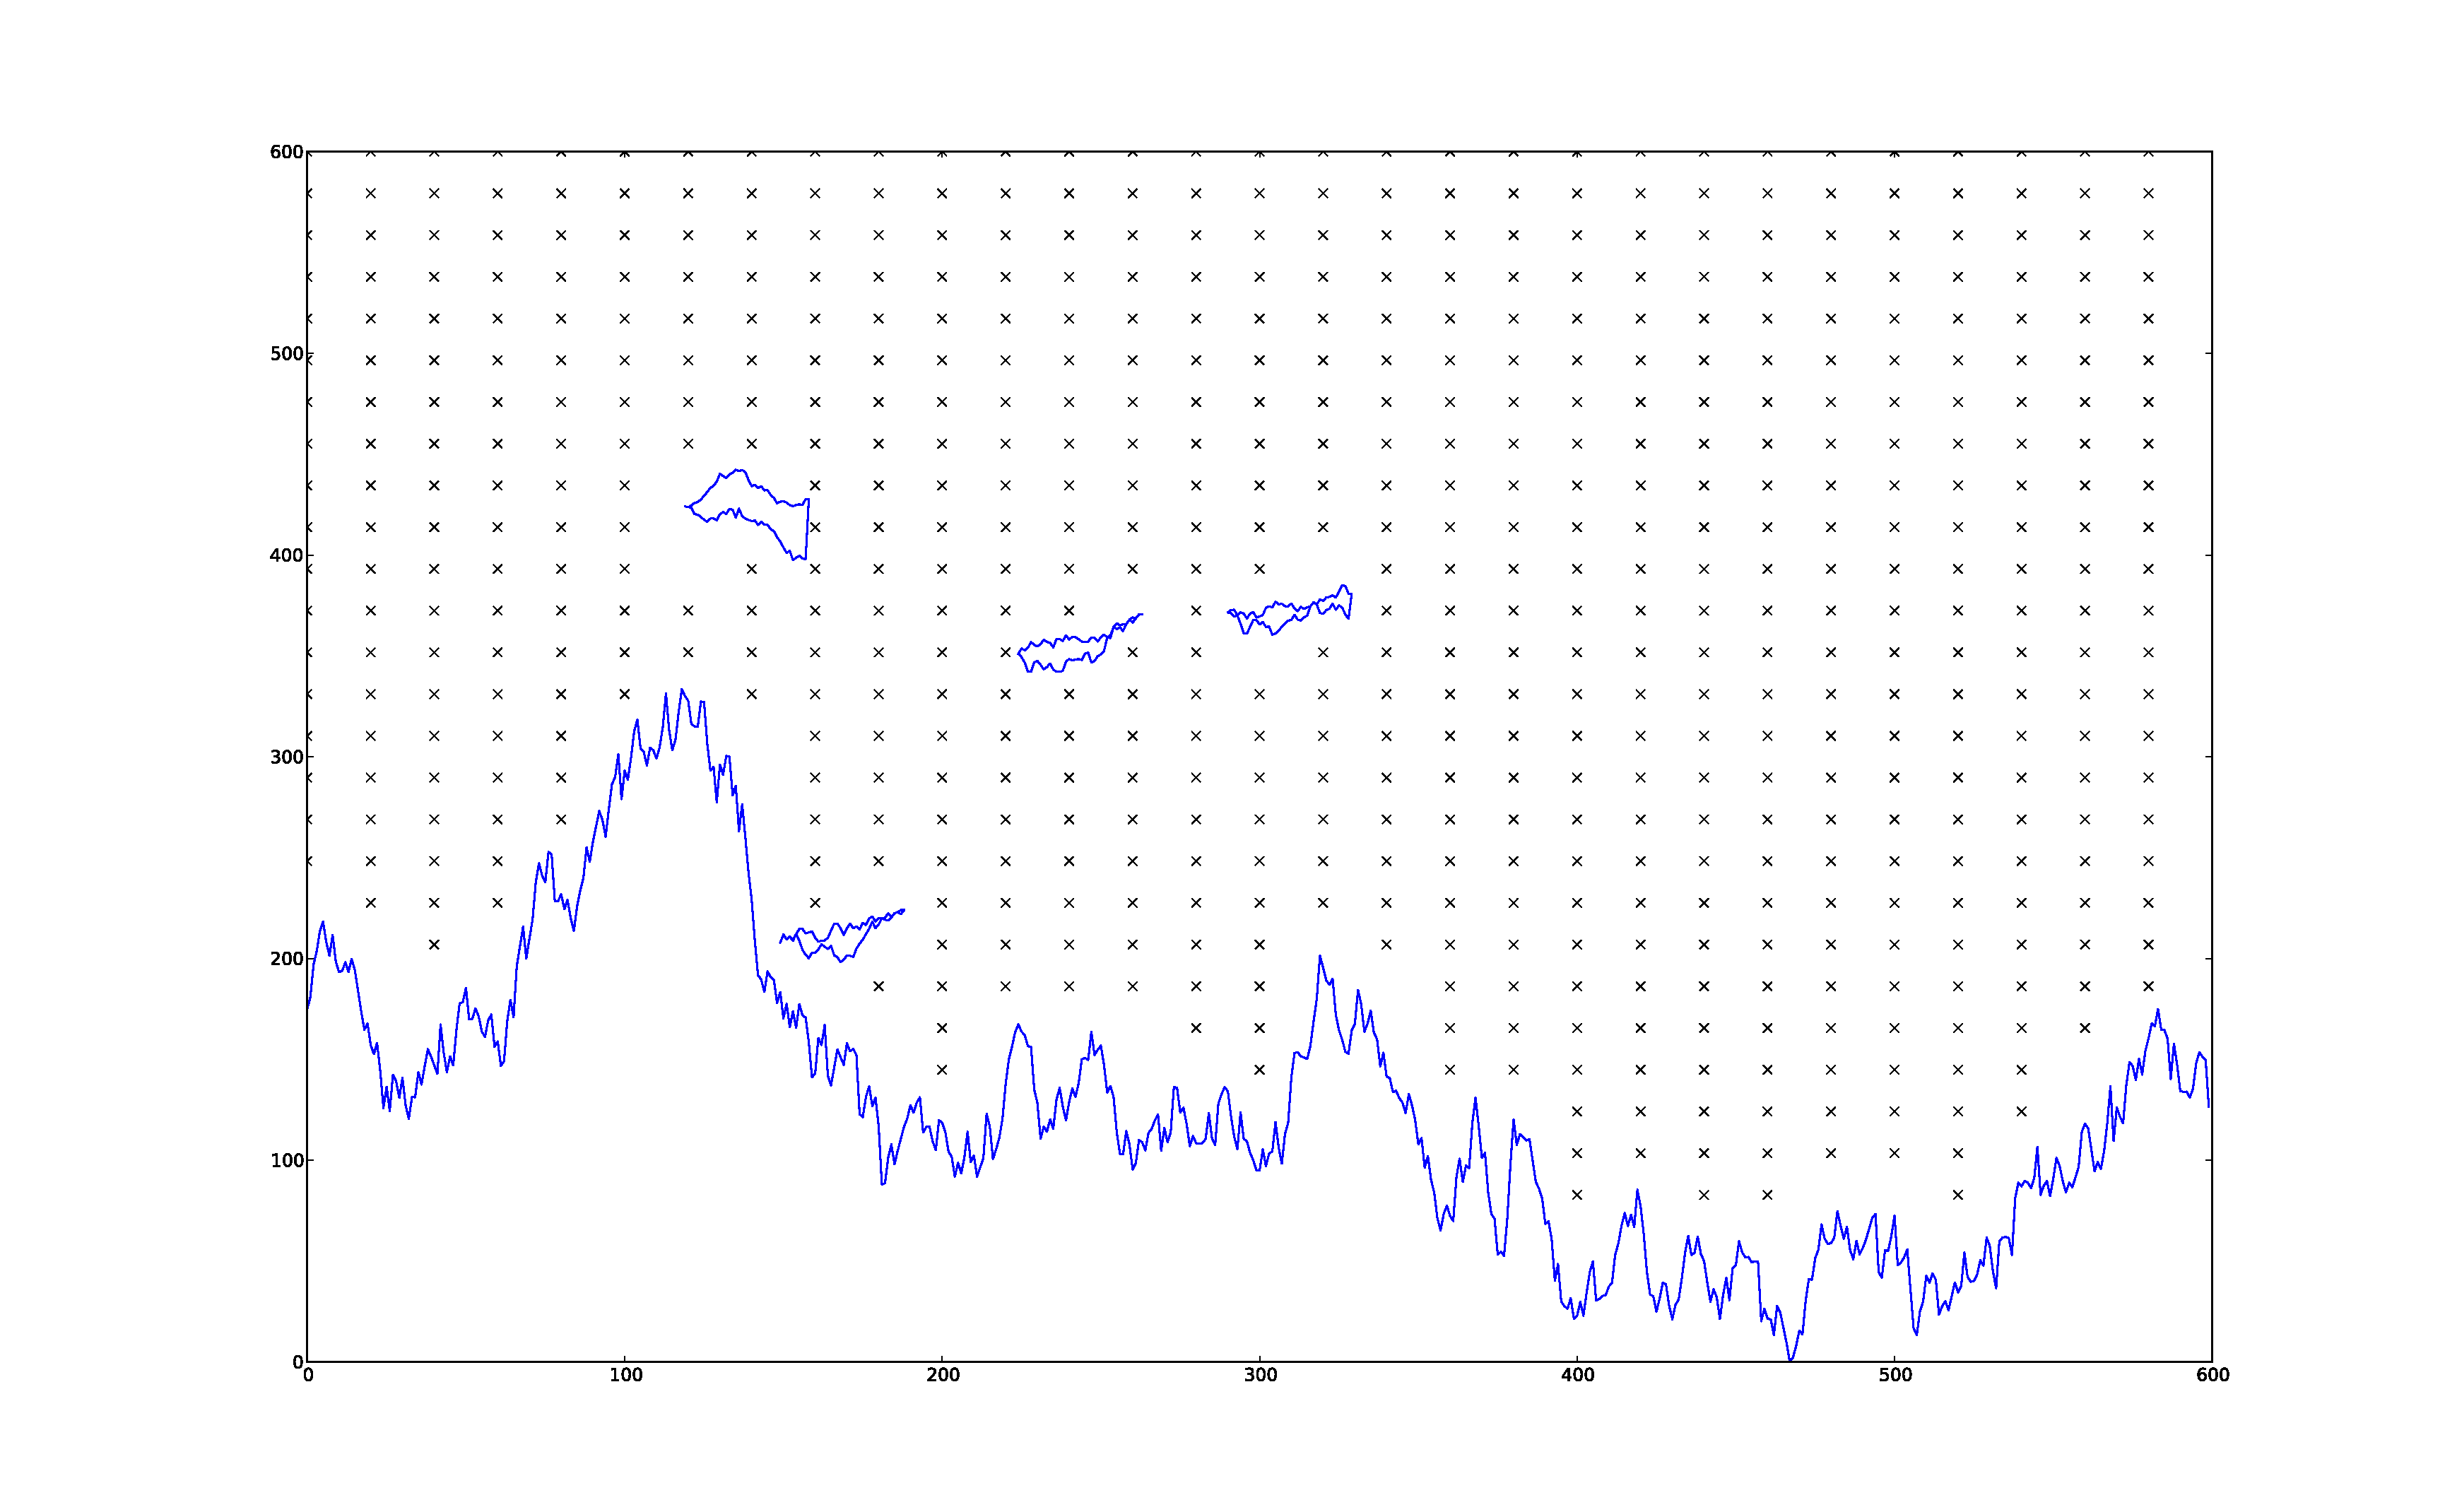
\includegraphics[width=0.8\textwidth]{img/linemap}
	\caption{The coastlines}
	\label{fig:linemap}
\end{figure}

The generated coastlines are converted to the actual Map, which is a number of surfaces: Figure~\ref{fig:solidmap}.

\begin{figure}[H]
	\centering
	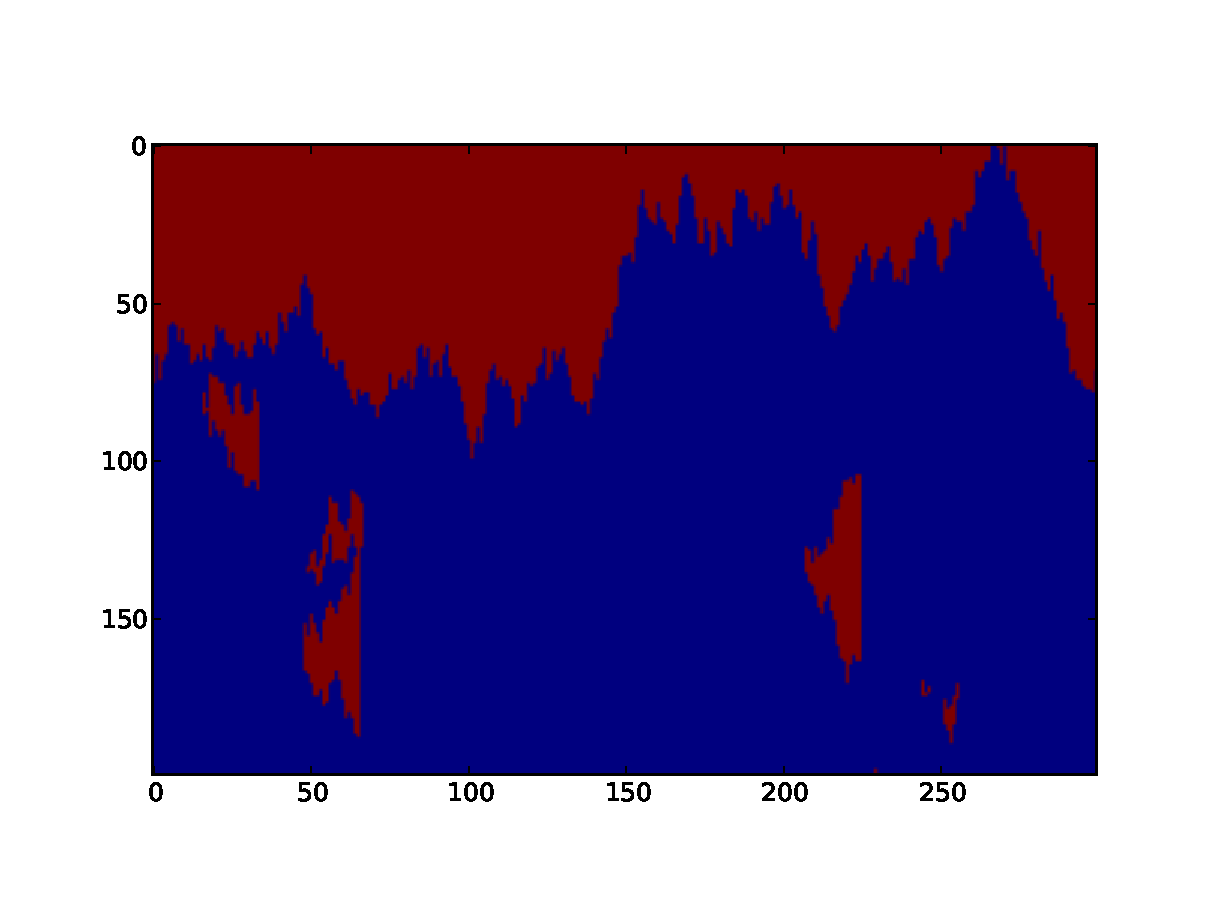
\includegraphics[width=\textwidth]{img/solidmap}
	\caption{The solidified map (the picture shows a north ("upside down") coast)}
	\label{fig:solidmap}
\end{figure}

Reading a solid map is possible from image files as well, using the Python SciPy library

\begin{figure}[H]
	\centering
	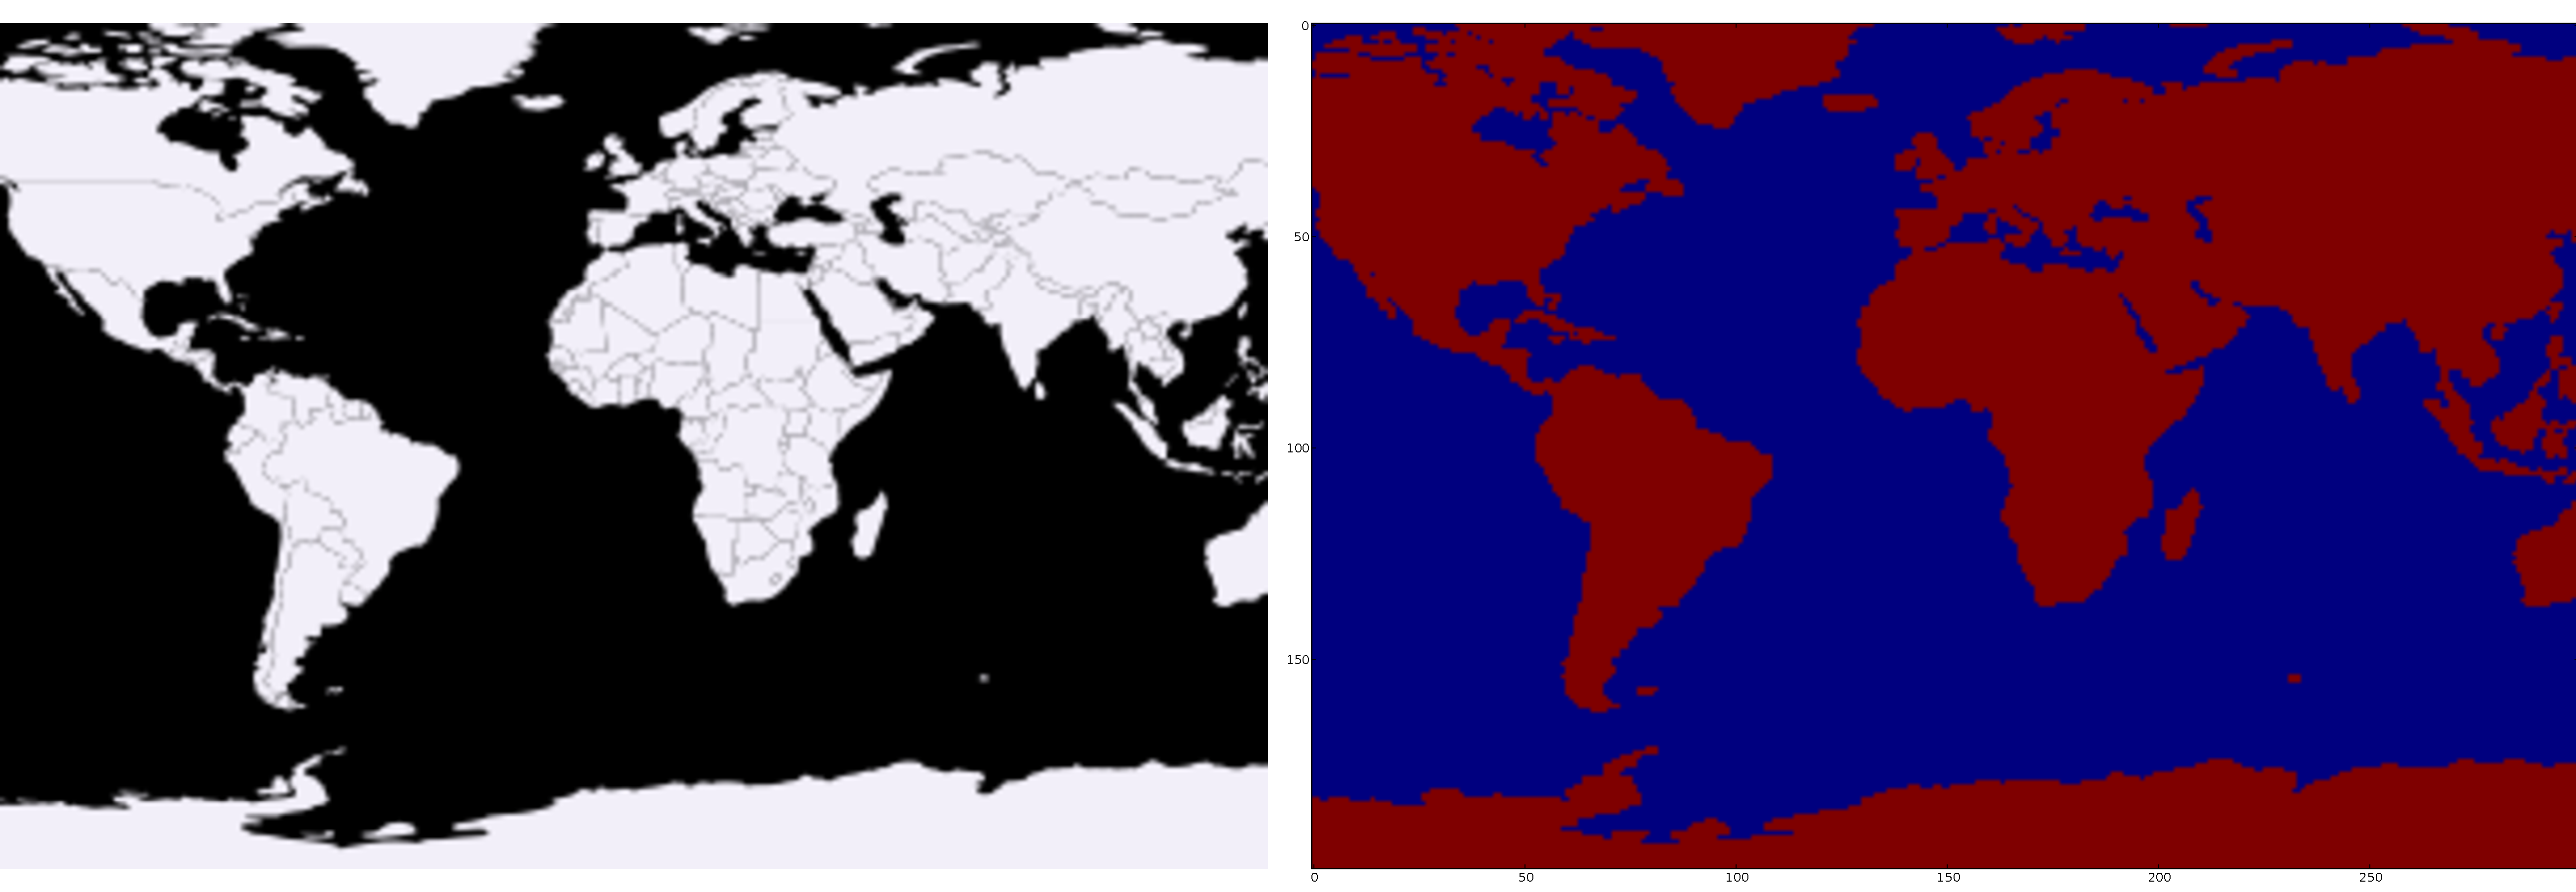
\includegraphics[width=0.8\textwidth]{img/worldmap}
	\caption{Image file processed to Map object}
	\label{fig:worldmap}
\end{figure}

\section{Routing}

Upon entering the water, the first task of the vessel in automatic or autonomus mode is to determine the course. Currently the software can not handle rivers, strong wind and magnetic declination, therefore the course is assumed to be identical to the heading.

\paragraph{The Waypoint planner} is responsible for the generating and ordering of the key measurement points. Visiting a set of waypoints on a given map leads to the Traveling Salesman NP-complete problem. Even using dynamic programming, determining the best route with the Held-Karp algorithm the program requires $O(N^2 2^2)$ steps [wiki]. The problem has been in the crosshair of mathematics for a long time, but a fast exact solution has never been found. The waypoint-planning is not time-critical, but a sufficient length of path should be calculated in a reasonable amount of time.

Fortunately the arrangement of the measurement points is relatively dense and predictable, allows only neighboring travels and repeated visits. In order to reach a suitable algorithm, some heuristics of the path planning needs to be examined.

\begin{tcolorbox}[colback=cyan!5,colframe=cyan!40!black,title=Code: Ship.py \\ https://www.dropbox.com/s/fmtsaatql7jqjhw/Ship\texttt{\_}nofilter.py]
\begin{minipage}{0,6\textwidth}
Ship.py implements the Ship Object. Everything related to the handling of a ship is encapsulated in a Ship instance. Multiple instances can be created based on the same object, with different parameters, and they are using the same resources.
\end{minipage}
\begin{minipage}{0,35\textwidth}
\raggedleft

\includegraphics[width=0.8\textwidth]{img/ship}
\end{minipage}
\end{tcolorbox}

\paragraph{In a simple coastline} the points can be placed in a certain order relative to the coast, to achieve a sufficient result. If the shore is relatively smooth, the ship can also travel parallel to the coast, to decrease the required number of turns.

\begin{figure}[H]
	\centering
	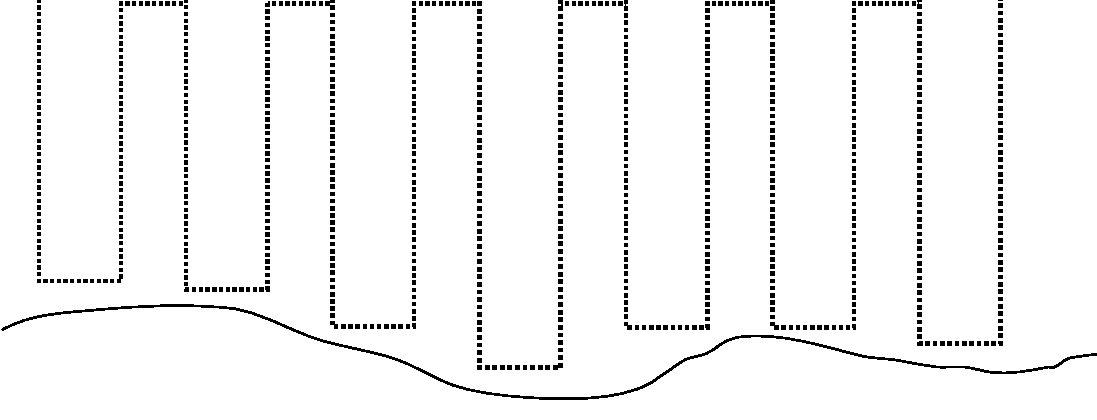
\includegraphics[width=\textwidth]{img/simplecoast}
	\caption{A simple coast and a sufficient path}
	\label{fig:simplecoast}
\end{figure}

\paragraph{Introducing isles and deep bays} to the area complicate the situation. Some waypoints need to be removed, and an avoiding path needs to be taken. This will cause many redundant measurements and very sub-optimal path, if the island density and the complexity of the coast is high.

\begin{figure}[H]
	\centering
	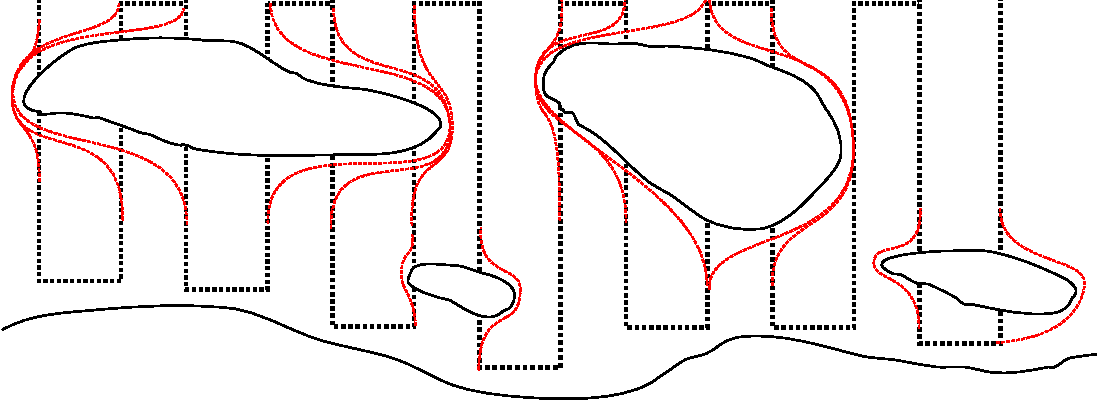
\includegraphics[width=\textwidth]{img/pathislands}
	\caption{Coast with islands}
	\label{fig:pathislands}
\end{figure}

\paragraph{Greedy traversal}

stretches a measurement grid over the area, and the points are traversed in an unpredictable way, using a neirest neighbourgh algorithm.

\begin{figure}[H]
	\centering
	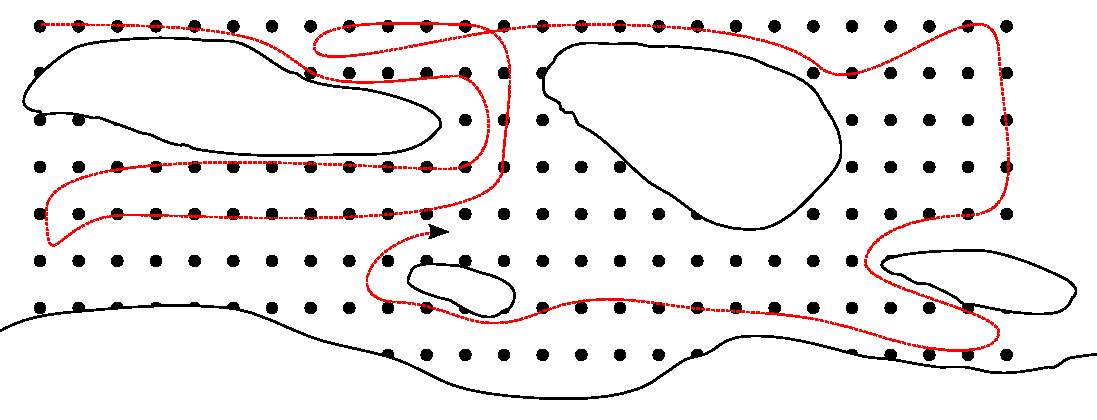
\includegraphics[width=\textwidth]{img/traversal}
	\caption{A random path based on graph traversal}
	\label{fig:traversal}
\end{figure}

 According to [citation] heuristic closest neighbour search is usually 5-10\% worse than the ideal solution. Using the closest neighbour heuristic, the simulation leads to the following path: Figure~\ref{fig:nn}.

\begin{figure}[H]
	\centering
	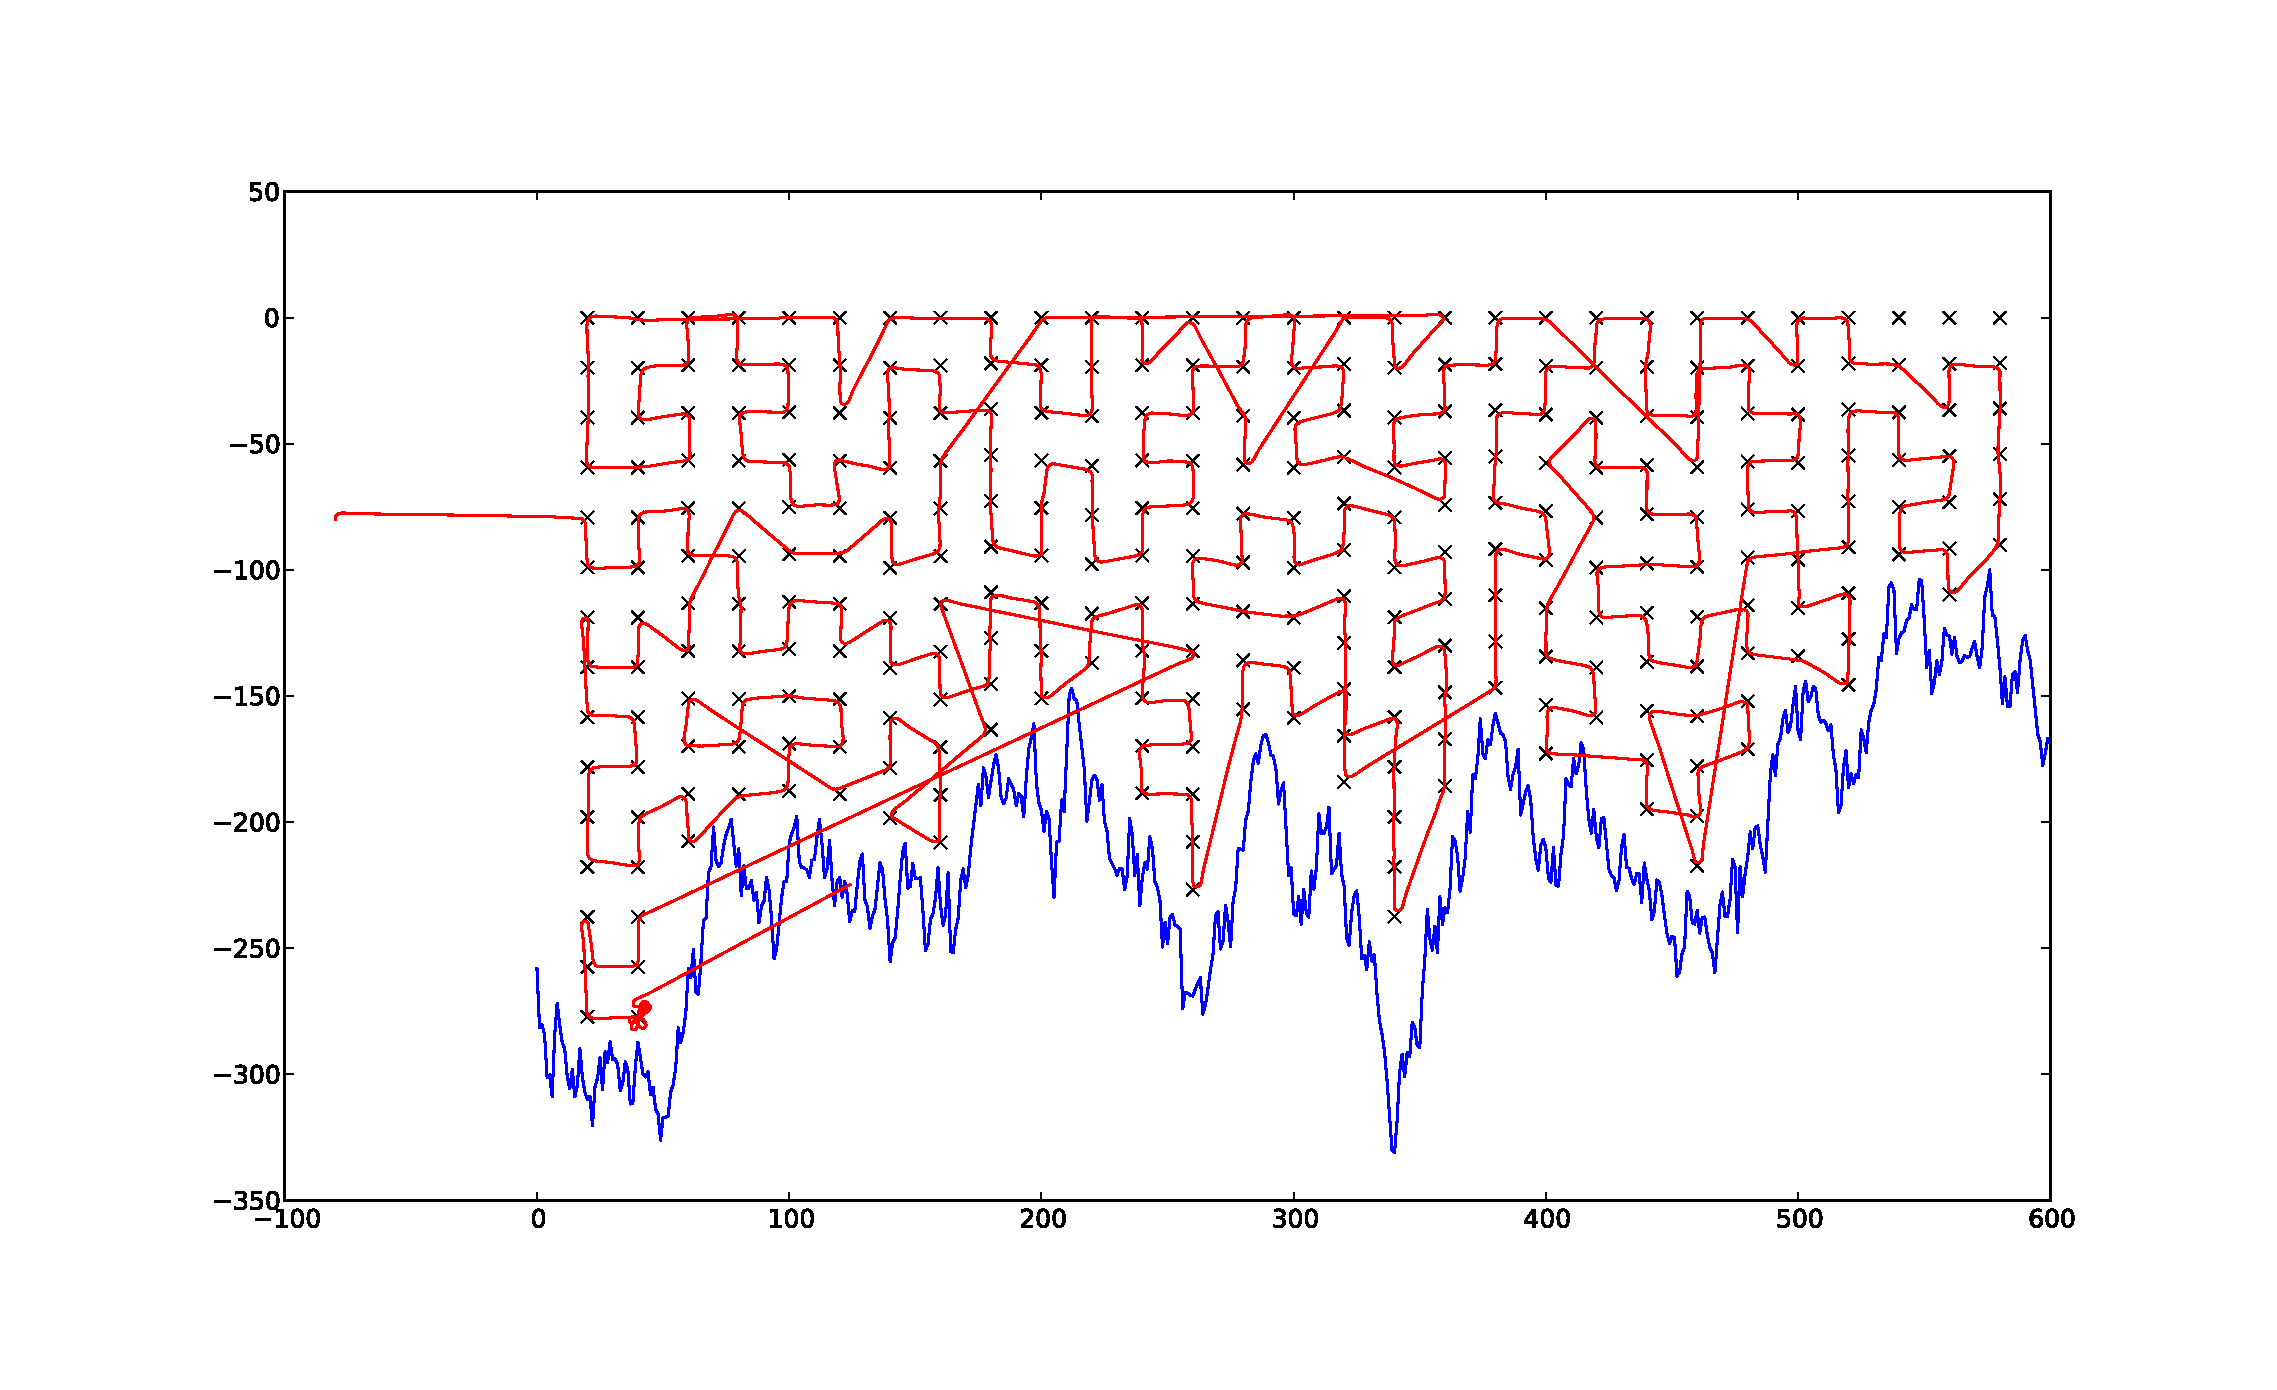
\includegraphics[width=\textwidth]{img/nn}
	\caption{Neirest neighbourgh algorithm}
	\label{fig:nn}
\end{figure}

\subsection{Lowest cost heuristics}

Even without major nautical engineering skills the following presumption can be made: If there are two paths with identical start and finish and identical lengths (start != finish) the  path with less turning is more effective.
This presumption can be extended to the following theory:

The most effective nautical path between two given points is the one with the least sum cost. The sum cost is the traveled distance times distance cost, plus absolute turnining times turning cost.

\begin{align}
	\Sigma C  = dist*C_{dist} + |turn| * C_{turn}
\end{align}

The cost of the distance and the turning depends on the type of the ship. A large, deep draught cargo ship capable of low speed will have a much higher $\frac{Distance}{Turn}$ cost ratio than a narrow military cruiser.


Using the considerations above a cost based nearest neighbour algorithm is introduced, where the lowest distance is replaced with lowest cost. The algorithm checks every point to determine which is the cheapest destination. To avoid path-loops in the map, the waypoints already visited are stored in a list. If the examined point is already in the list, the cost is increased with a redundancy value, so the algorithm will chose a different, slightly more expensive, but still unvisited measurement point. The algorithm also checks, if the path leading to the examined waypoint is clear of obsticles.

Running the simulation with the above pathplanner results in the following course: Figure~\ref{fig:lc}.

\begin{figure}[H]
	\centering
	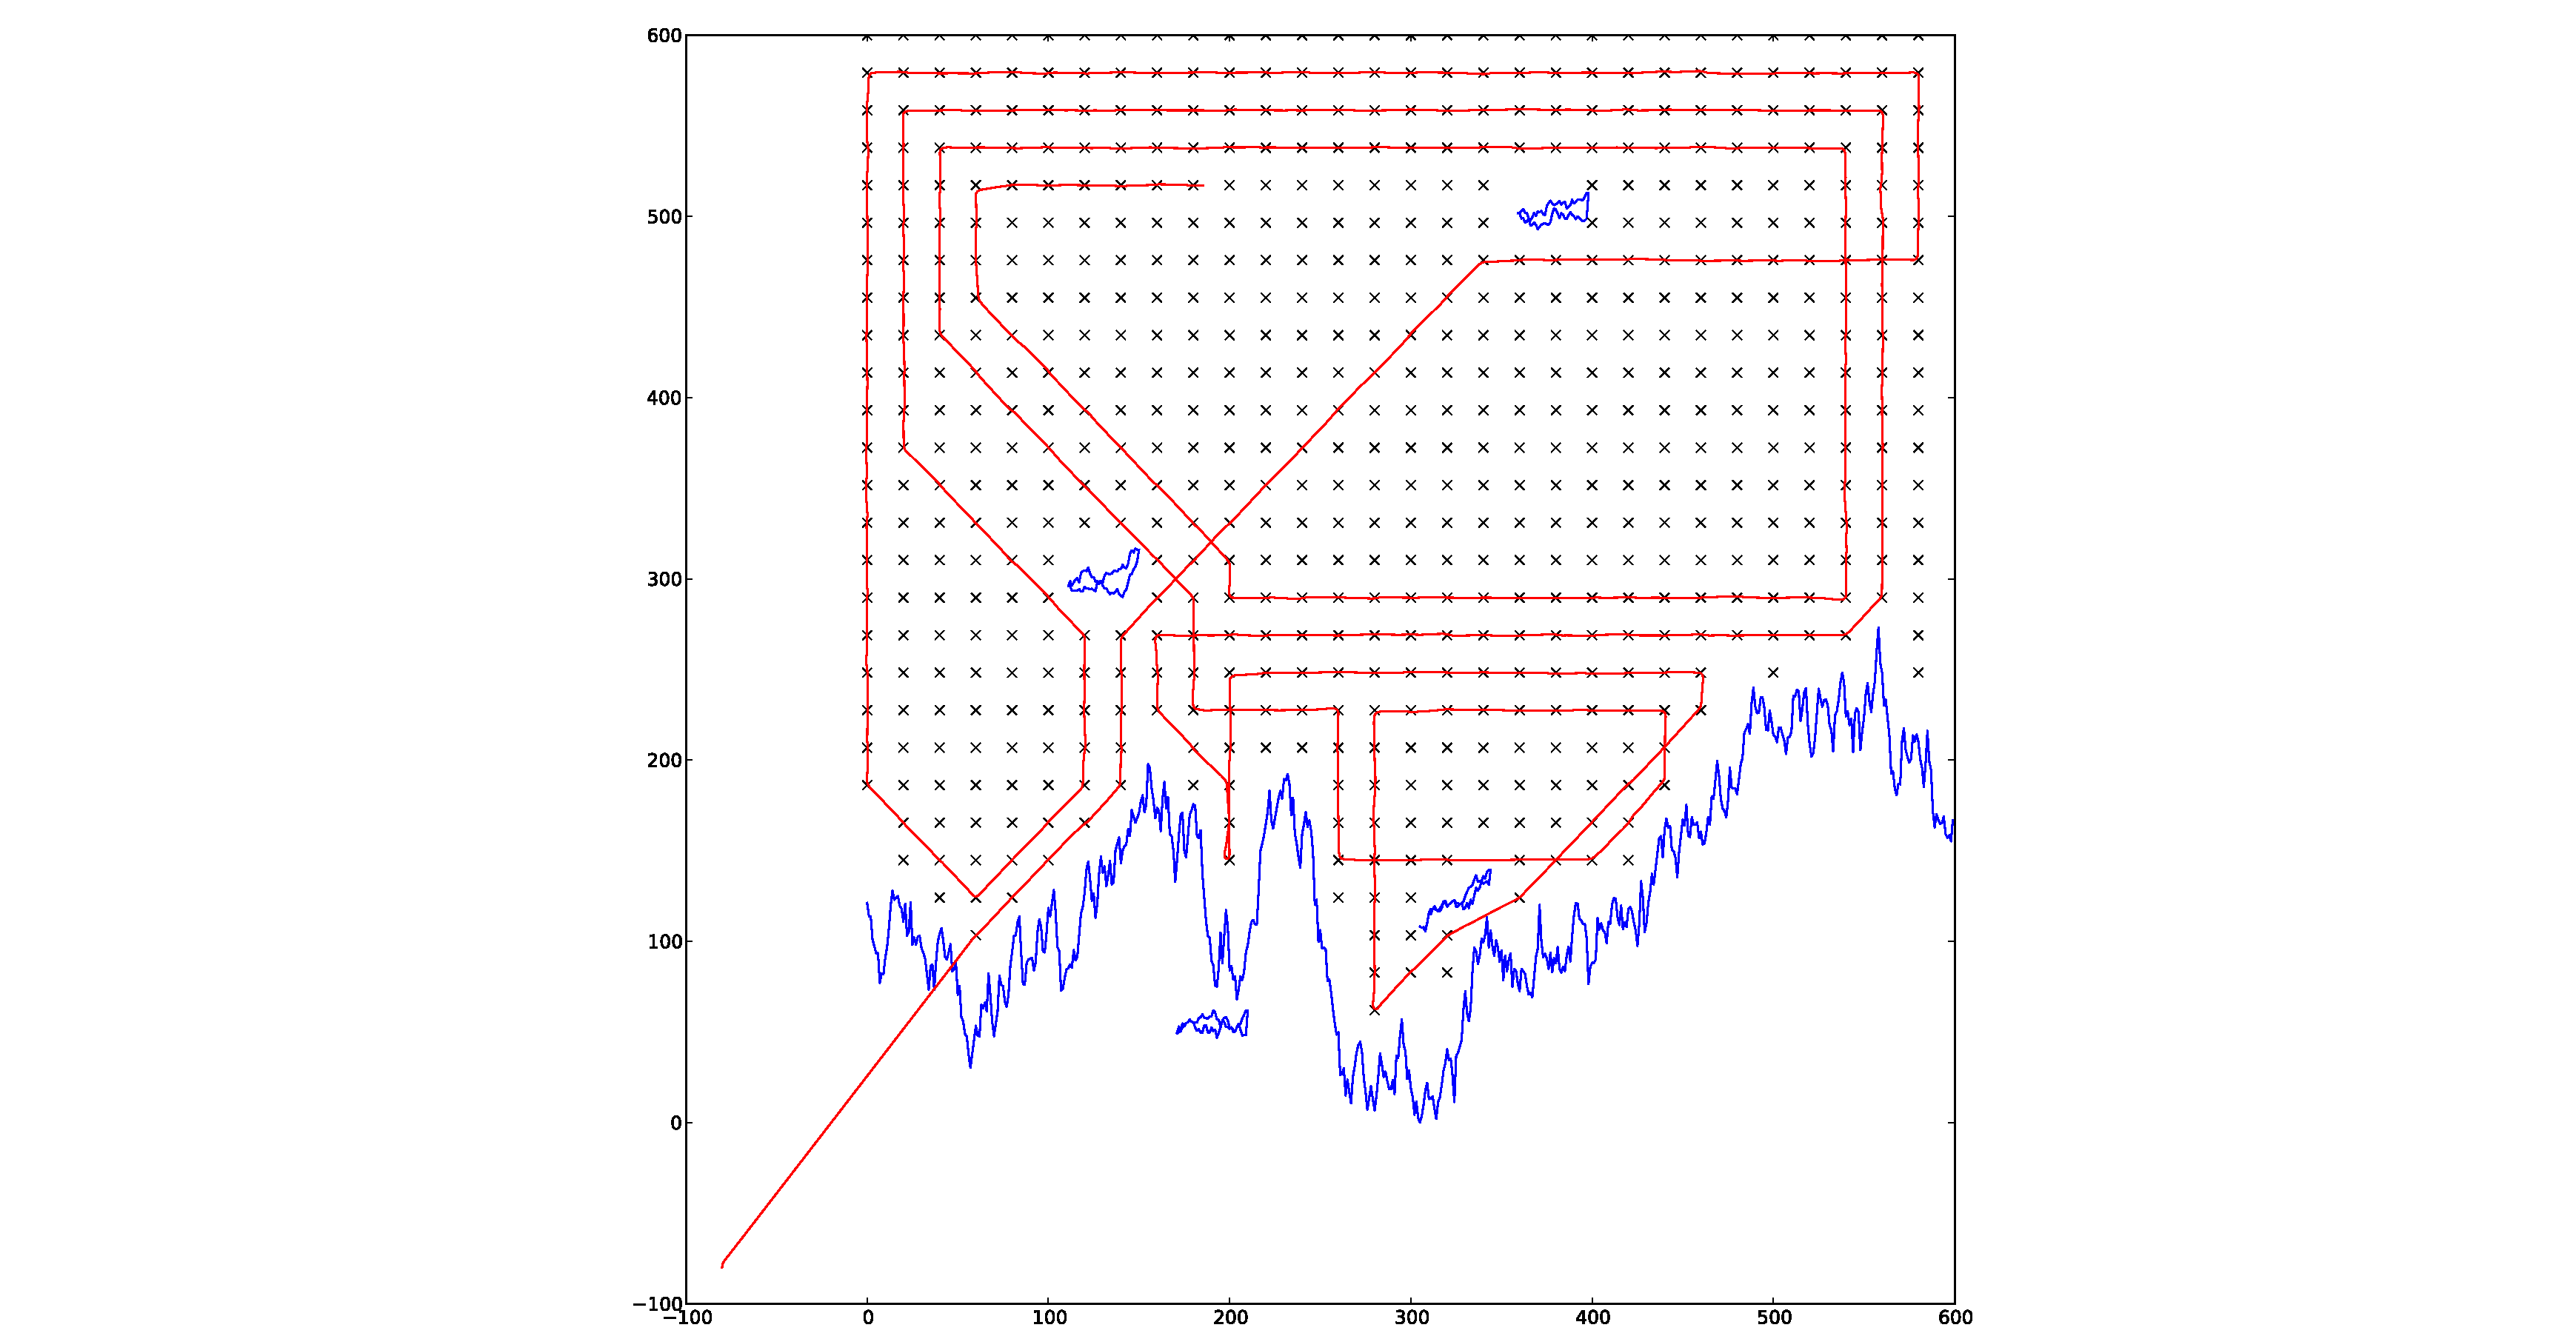
\includegraphics[width=\textwidth]{img/geee}
	\caption{Lowest cost algorithm}
	\label{fig:lc}
\end{figure}

This navigation method works adequatly in open environments. However, if the map is consisted of tight narrows and hard to navigate areas, the algorithm above fails to exit certain areas of the map. To be able to operate in such shores, a different kind of routing is required.

I call this method "Ripple", because the points examined are moving away from the surface vessel in a circular shape (well, in a rectangular actually) like a ripple. The ripple checks every neighbouroing waypoint, that wasnt checked so far, and stores the previous life of the ripple. If a point is found that has not been visited before, a list of waypoints are returned, and the ship will sail through them, and reach the destination.

Figure~\ref{fig:ripple} illustrates this navigation method by simulating a task on the map of the Earth.

\begin{figure}[H]
	\centering
	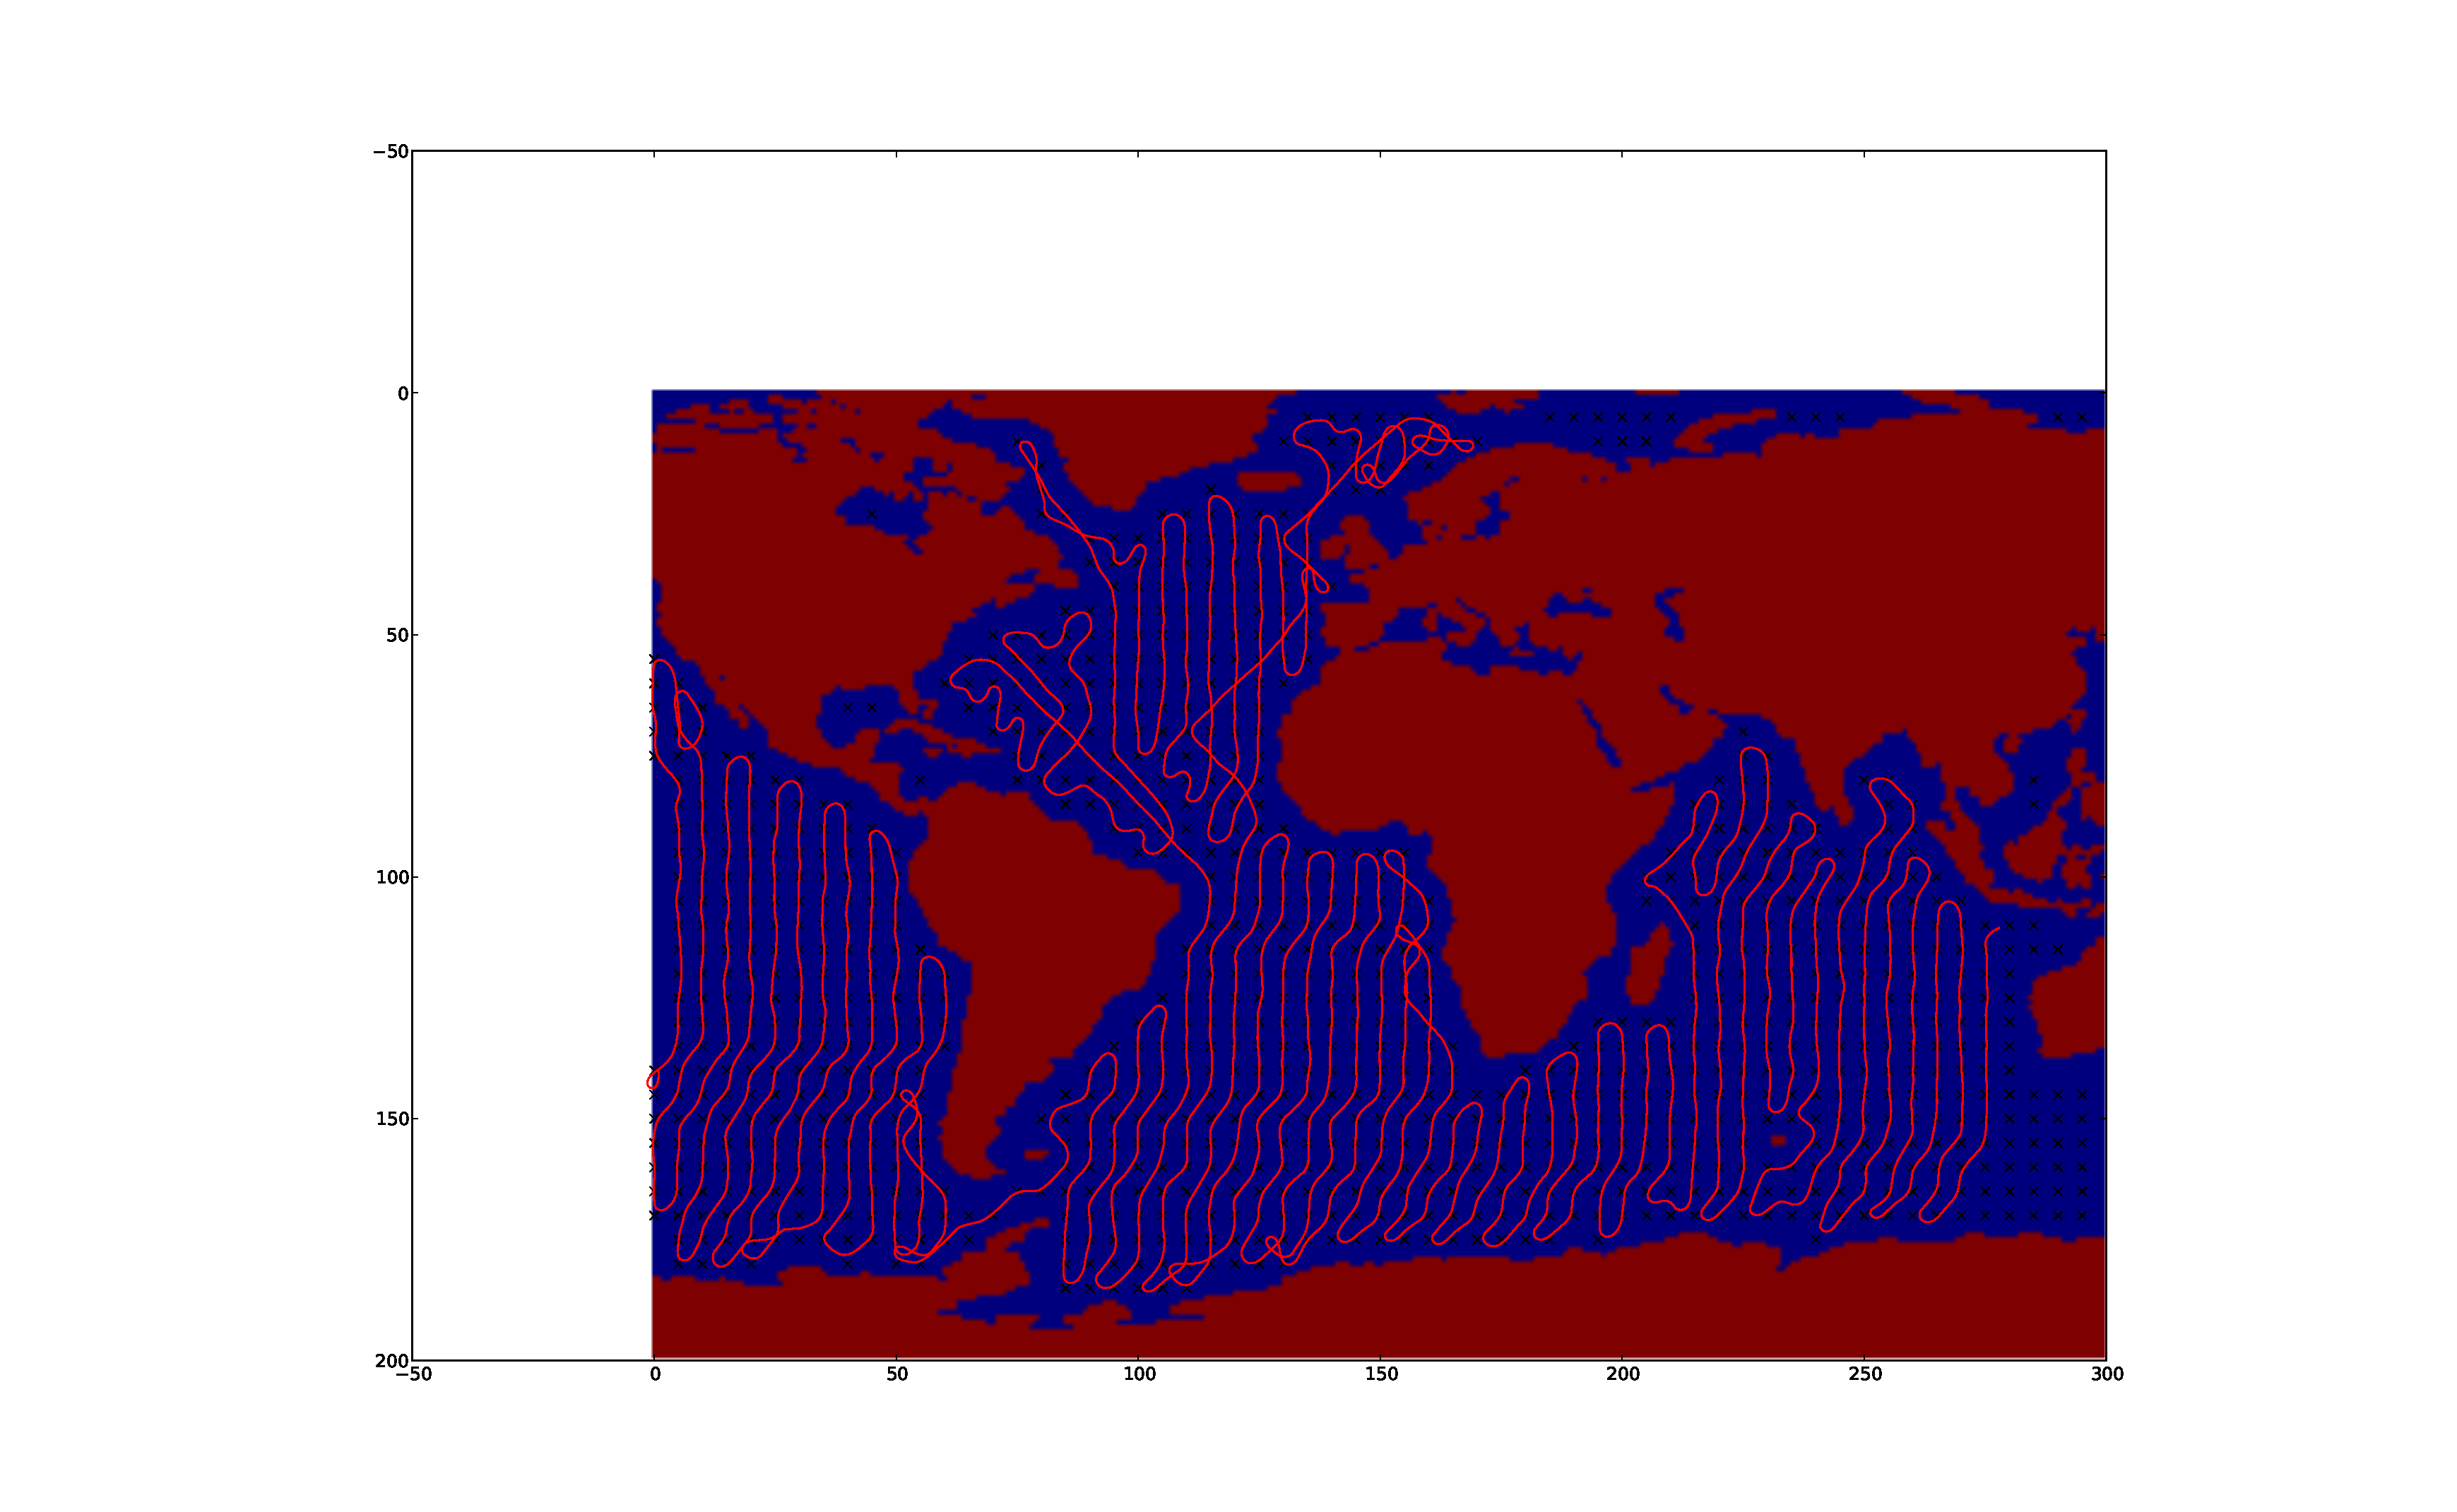
\includegraphics[width=\textwidth]{img/ripple}
	\caption{Ripple routing algorithm}
	\label{fig:ripple}
\end{figure}

\section{Navigation}

Once the required course has been set, the control system will take over the handling of the ship. The Navigation is the first and highest layer of control in the High Level Controller. In order to explain the navigation, the coordinate systems must be defined first.

\subsection{Frames of reference}

The operator team and the GPS sensor are using the Earth Centered Earth Fixed (ECEF) coordinate systems. Navigation on a spherical surface would introduce a lot of unnecessary calculations in every control cycle, since a plane can be fit onto the surface with minimal error, because the small vessel has limited maximum range.

During the Navigation the North East Down coordinate system is used to determine the attitude and position of the ship. The NED coordinate system is centered to the first GPS measurement coordinate.

A third Body Frame is also defined, the dynamic system of the ship was calculated in this frame.

\begin{figure}[H]
	\centering
	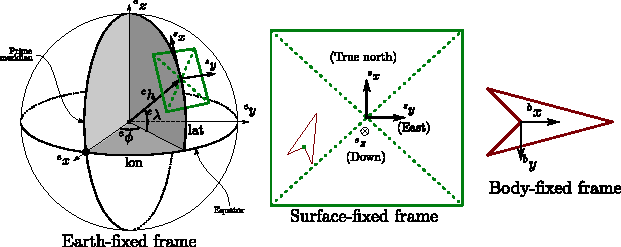
\includegraphics[width=\textwidth]{img/reference_frames}
	\caption{Used coordinate systems}
	\label{fig:coordinatesystem}
\end{figure}

\begin{align}
	\lambda = longitude  \quad \phi = latitude
	\\ GPS_{[\lambda , \phi , h]} \Longleftrightarrow [X_{NED}; Y_{NED}; Z_{NED}]
\end{align}

\subsection{Required heading}

The heading of the ship is defined in NED coordinate system. The required heading is determined by the Law of Cosines, based on the Position of the Ship and the Position of the next Sub-Waypoint.
\begin{center}
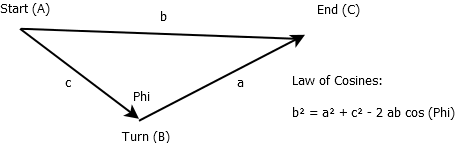
\includegraphics[scale = 0.4]{img/Law_of_Cosines}
\end{center}
Problems rise and corrections are necessary, if the heading of the ship $\theta$ is $\theta < -\pi$ or $\theta < \pi$. The heading of the ship is calculated based on the Gyro sensor and the heading can have any value in the form of: 
\begin{align}
\theta = [-{\pi} ; \pi ] \pm 2 \cdot k \cdot \pi
\end{align}\\

\begin{tcolorbox}[colback=cyan!5,colframe=cyan!40!black,title=Code: FunctionLibrary.py \\ https://www.dropbox.com/s/7nx7helisvss21a/FunctionLibrary.py]
\begin{minipage}{0,6\textwidth}
Some functions required by the software are general parametric mathematical functions, which can not be connected to any object. These functions, like the Law of Cosines, and the distance calculator function can be found in the Function Library.
\end{minipage}
\begin{minipage}{0,35\textwidth}
\raggedleft

\includegraphics[width=0.8\textwidth]{img/functionlibrary}
\end{minipage}


\end{tcolorbox}

Before invoking the control procedure, all of the heading angles must be transformed into the $[-\pi ; \pi]$ interval.
This procedure causes a possible error though.

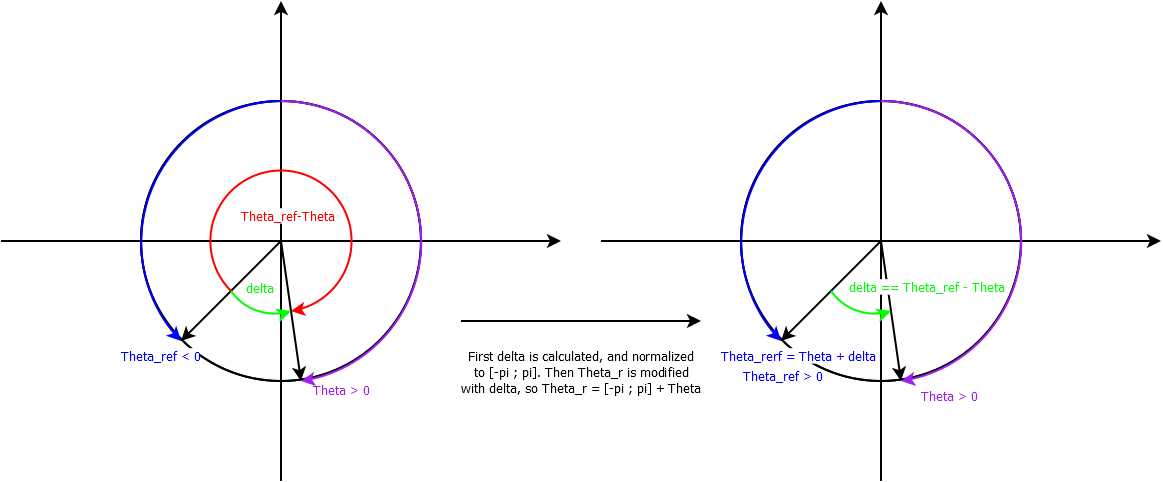
\includegraphics[width=\textwidth]{img/Headings}

The required heading or the heading of the ship must be transformed into a different representation, where 
\begin{align}
|\theta_{r}-\theta| < \pi
\end{align}
To keep a consistent heading representation, first the deviation angle 
\begin{align}
\theta = \pi_{r}-\pi
\end{align} is calculated, than transformed to the $[-\pi;\pi]$ interval and finally, with $\delta$ we can transform $\theta_{r}$ to 
\begin{align}
\theta_{r}(\theta) = \theta + \delta
\end{align}
If the conditions above are met, $\theta$ and $\theta_r(\theta)$ will always yield values that result in correct controller output.

\subsection{Waypoint planning}

\subsection{Waypoint ordering}

\subsection{Comparsion of methods (length/WP)}

\subsection{Map reading}
\section{Swarm intelligence}
\section{Measurements and results}
\section{Conclusion}
This document is meant to succeeds my previous work\cite{aau}. Several major functionalities have been added, and the engine behind under the hood has been changed, and will keep changing.

My most important observation during the Project Laboratory I. was that the perceived significance of the system components might differ from the reality. The successful implementation of the different pathplanning systems and navigation required a very solid and relatively simple Map object, that can be relied on.

With the major components of the HLC now complete, up and running, it's possible to move to the next phase. In Project Laboratory II. the LLC will be designed, the communication protocol between the objects and the ship itself, in order to accomplish a more-or-less working prototype by the end of 2013.
%----------------------------------------------------------------------------
%\chapter*{Köszönetnyilvánítás}\addcontentsline{toc}{chapter}{Köszönetnyilvánítás}
\section{Acknowledgment}
%----------------------------------------------------------------------------

Ez nem kötelező, akár törölhető is. Ha a szerző szükségét érzi, itt lehet köszönetet nyilvánítani azoknak, akik hozzájárultak munkájukkal ahhoz, hogy a hallgató a szakdolgozatban vagy diplomamunkában leírt feladatokat sikeresen elvégezze. A konzulensnek való köszönetnyilvánítás sem kötelező, a konzulensnek hivatalosan is dolga, hogy a hallgatót konzultálja.
%%----------------------------------------------------------------------------
\appendix
%----------------------------------------------------------------------------
%\chapter*{Függelék}\addcontentsline{toc}{chapter}{Függelék}
\section{Appendices}

\setcounter{section}{6}  % a fofejezet-szamlalo az angol ABC 6. betuje (F) lesz
\setcounter{equation}{0} % a fofejezet-szamlalo az angol ABC 6. betuje (F) lesz
\numberwithin{equation}{subsection}
\numberwithin{figure}{subsection}
\numberwithin{lstlisting}{subsection}
%\numberwithin{tabular}{section}

%----------------------------------------------------------------------------
\section{A TeXnicCenter felülete}
%----------------------------------------------------------------------------
\begin{figure}[!ht]
\centering
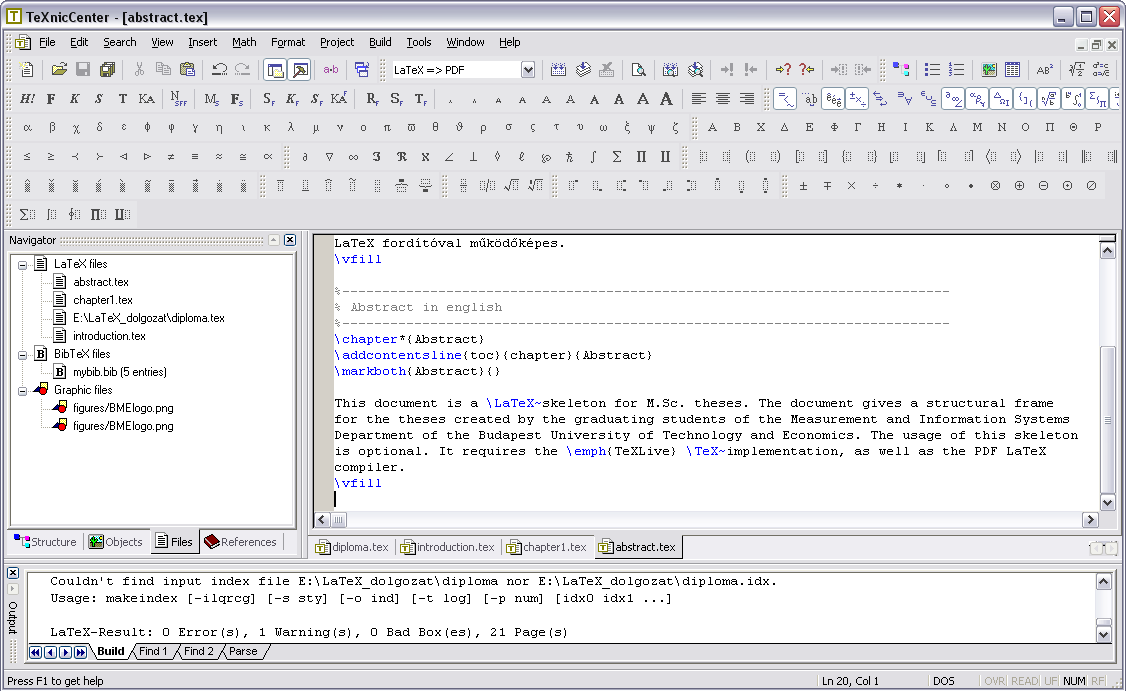
\includegraphics[width=150mm, keepaspectratio]{figures/TeXnicCenter.png}
\caption{A TeXnicCenter Windows alapú \LaTeX-szerkesztő.} 
\end{figure}

%----------------------------------------------------------------------------
\clearpage\section{Válasz az ,,Élet, a világmindenség, meg minden'' kérdésére}
%----------------------------------------------------------------------------
A Pitagorasz-tételből levezetve
\begin{align}
c^2=a^2+b^2=42.
\end{align}
A Faraday-indukciós törvényből levezetve
\begin{align}
\rot E=-\frac{dB}{dt}\hspace{1cm}\longrightarrow \hspace{1cm}
U_i=\oint\limits_\mathbf{L}{\mathbf{E}\mathbf{dl}}=-\frac{d}{dt}\int\limits_A{\mathbf{B}\mathbf{da}}=42.
\end{align}







%\listoffigures\addcontentsline{toc}{chapter}{Ábrák jegyzéke}
%\listoftables\addcontentsline{toc}{chapter}{Táblázatok jegyzéke}

\bibliography{bibl}
\addcontentsline{toc}{section}{Bibliography}
\bibliographystyle{unsrt}

%----------------------------------------------------------------------------
\appendix
%----------------------------------------------------------------------------
%\chapter*{Függelék}\addcontentsline{toc}{chapter}{Függelék}
\section{Appendices}

\setcounter{section}{6}  % a fofejezet-szamlalo az angol ABC 6. betuje (F) lesz
\setcounter{equation}{0} % a fofejezet-szamlalo az angol ABC 6. betuje (F) lesz
\numberwithin{equation}{subsection}
\numberwithin{figure}{subsection}
\numberwithin{lstlisting}{subsection}
%\numberwithin{tabular}{section}

%----------------------------------------------------------------------------
\section{A TeXnicCenter felülete}
%----------------------------------------------------------------------------
\begin{figure}[!ht]
\centering
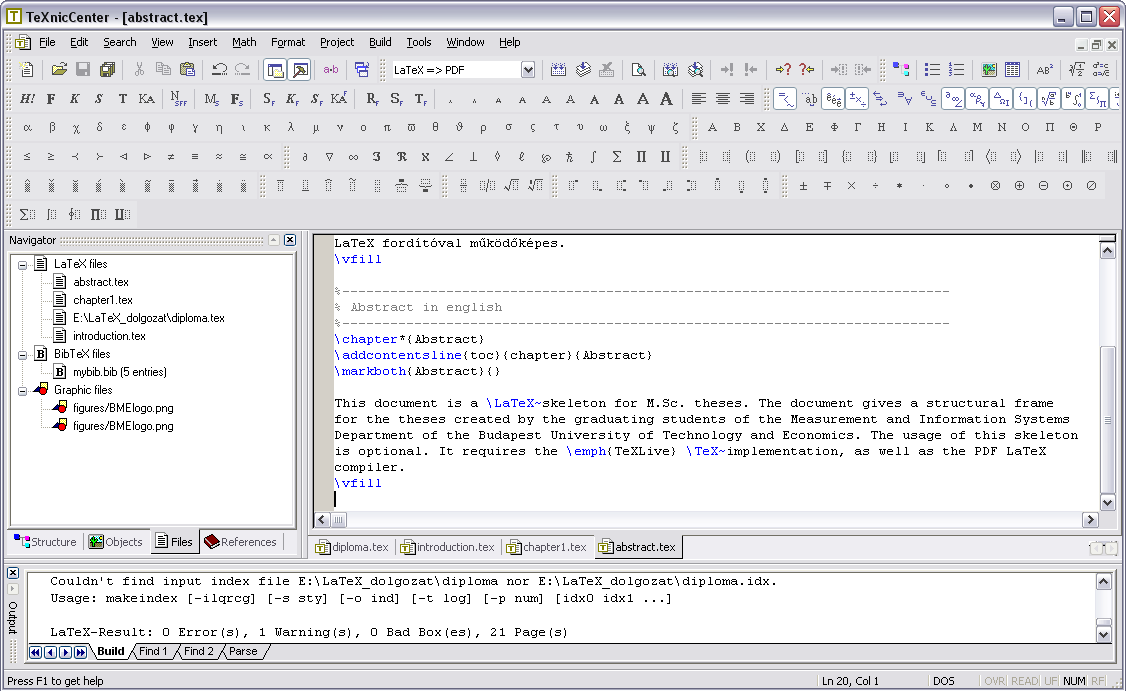
\includegraphics[width=150mm, keepaspectratio]{figures/TeXnicCenter.png}
\caption{A TeXnicCenter Windows alapú \LaTeX-szerkesztő.} 
\end{figure}

%----------------------------------------------------------------------------
\clearpage\section{Válasz az ,,Élet, a világmindenség, meg minden'' kérdésére}
%----------------------------------------------------------------------------
A Pitagorasz-tételből levezetve
\begin{align}
c^2=a^2+b^2=42.
\end{align}
A Faraday-indukciós törvényből levezetve
\begin{align}
\rot E=-\frac{dB}{dt}\hspace{1cm}\longrightarrow \hspace{1cm}
U_i=\oint\limits_\mathbf{L}{\mathbf{E}\mathbf{dl}}=-\frac{d}{dt}\int\limits_A{\mathbf{B}\mathbf{da}}=42.
\end{align}







\label{page:last}
\end{document}
